\باب{تفرقی ایمپلیفائر}

\حصہ{دو جوڑ ٹرانزسٹر کا تفرقی جوڑا}
\جزوحصہ{تفرقی اشارہ کی عدم موجودگی} 
شکل \حوالہ{شکل_تفرقی_جوڑے_کی_بنیادی_ساخت} میں دو جوڑ ٹرانزسٹر کا بنیادی \اصطلاح {تفرقی جوڑا}\فرہنگ{تفرقی!جوڑا}\فرہنگ{difference pair}\حاشیہب{difference pair} دکھایا گیا ہے۔\اصطلاح {تفرقی جوڑے} میں دو بالکل \اصطلاح {یکساں}\فرہنگ{یکساں}\حاشیہب{matched} ٹرانزسٹر  استعمال کئے جاتے ہیں۔تفرقی جوڑے کی صحیح کارکردگی کے لئے یہ ضروری ہے کہ  \عددی{Q_1} اور \عددی{Q_2}  افزائندہ خطے میں رہیں۔ انہیں افزائندہ خطے میں رکھنے کی خاطر تفرقی جوڑے کو \عددی{R_C} کی مدد سے منبع مثبت برقی دباو  \عددی{V_{CC}} کے ساتھ جوڑا گیا ہے۔جیسا کہ اسی باب میں بعد میں دکھایا جائے گا \عددی{R_C} کی جگہ ٹرانزسٹر بھی استعمال کئے جاتے ہیں۔تفرقی جوڑے کے دو داخلی اشارات \عددی{v_{B1}} اور \عددی{v_{B2}} ہیں جبکہ اس کا عمومی تفرقی خارجی اشارہ \عددی{v_o} ہے جسے شکل  \حوالہ{شکل_دونوں_مداخل_پر_برابر_برقی_دباو} میں دکھایا گیا ہے۔بعض اوقات \عددی{v_{C1}}  یا \عددی{v_{C2}}  کو ہی بطور خارجی اشارہ \عددی{v_o} لیا جاتا ہے۔

تفرقی جوڑے کے دونوں ٹرانزسٹروں کے ایمٹر سرے آپس میں جڑے ہونے کی وجہ سے ان دونوں سروں پر ہر صورت برابر برقی دباو ہو گا (یعنی \عددی{v_{E1}=v_{E2}} ہو گا) ۔ان برابر برقی دباو کو لکھتے ہوئے  زیرِ نوشت ( 1 اور 2 ) لکھے بغیر \عددی{v_E} لکھا جا سکتا ہے یعنی
\begin{align}
v_{E1}=v_{E2}=v_E
\end{align}
مزید یہ کہ اس جوڑ پر پیدا  کار برقی رو کی برقی رو \عددی{i_{E1}}  اور \عددی{i_{E2}} میں تقسیم ہو گی جس کے لئے کرخوف کے قانون برائے برقی رو کے تحت لکھا سکتا ہے
\begin{align} \label{مساوات_تفرقی_کل_رو_قطعی}
i_{E1}+i_{E2}=2 \times I
\end{align}
%
\begin{figure}
\centering
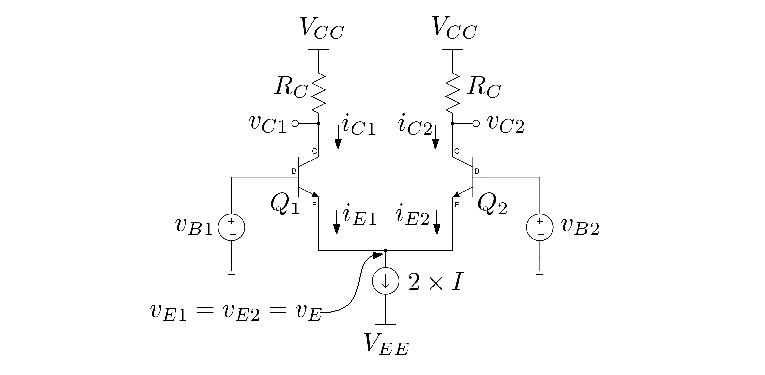
\includegraphics[scale=0.90]{differencePair}
\caption{دو جوڑ ٹرانزسٹر کے تفرقی جوڑے کی بنیادی ساخت}
\label{شکل_تفرقی_جوڑے_کی_بنیادی_ساخت}
\end{figure}
%
تفرقی جوڑے کی کارکردگی پر شکل \حوالہ{شکل_دونوں_مداخل_پر_برابر_برقی_دباو} کی مدد سے غور کرتے ہیں جہاں تفرقی جوڑے کے دونوں داخلی سروں پر یک سمت برقی دباو \عددی{V_B}   بطور داخلی اشارات \عددی{v_{B1}} اور \عددی{v_{B2}}  مہیا کیا گیا ہے۔یوں \عددی{V_B} کو بطورِ \اصطلاح {مشترکہ برقی دباو}\فرہنگ{مشترکہ برقی دباو}\فرہنگ{common mode voltage}\حاشیہب{common mode voltage}  مہیا کیا گیا ہے۔ دور کو دیکھتے ہوئے یہ بات واضح ہے کہ اس کے بائیں اور دائیں اطراف بالکل یکساں ہیں۔یوں دونوں اطراف میں برابر برقی رو پائی جائے گی (یعنی \عددی{i_{E1}=i_{E2}})۔ایسی صورت میں مساوات \حوالہ{مساوات_تفرقی_کل_رو_قطعی}  سے \عددی{i_{E1}=i_{E2}=I}   حاصل ہوتا ہے اور یوں \عددی{i_{C1}=i_{C2}=\alpha I} ہو گا۔لہٰذا
\begin{align*}
v_{C1}&=V_{CC}-i_{C1} R_C=V_{CC}-\alpha I R_C\\
v_{C2}&=V_{CC}-i_{C2}R_C=V_{CC}-\alpha I R_C
\end{align*}
%
\begin{figure}
\centering
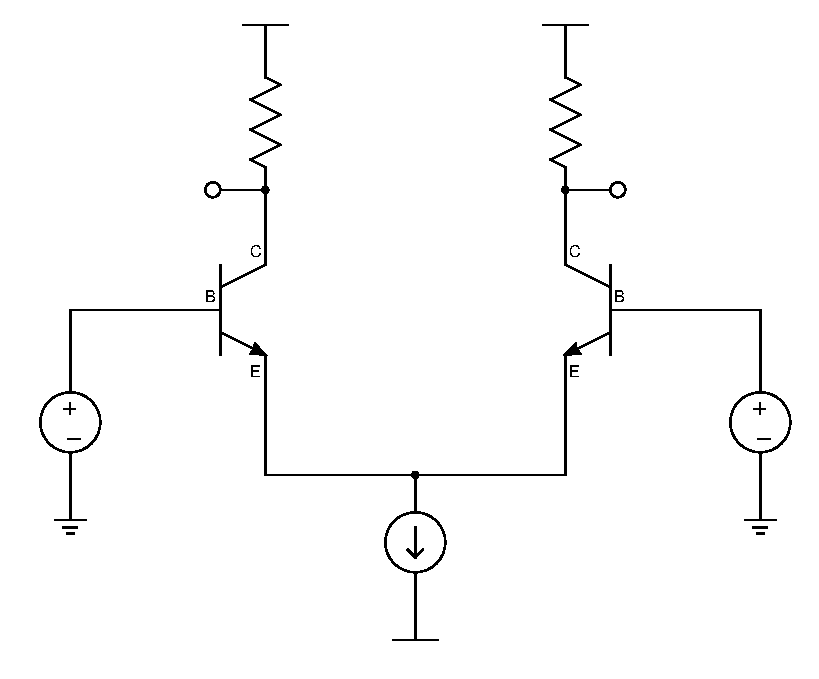
\includegraphics[scale=0.90]{differencePairCommonSignal}
\caption{ دونوں مداخل پر برابر برقی دباو کی صورت}
\label{شکل_دونوں_مداخل_پر_برابر_برقی_دباو}
\end{figure}
اس صورت میں
\begin{align}
v_o=v_{C2}-v_{C1}=0
\end{align}
ہو گا۔ یہ ایک اہم اور عمومی نتیجہ ہے جس کے تحت اگر تفرقی جوڑے کے دونوں مداخل پر برابر برقی دباو مہیا کیا جائے تو یہ صفر وولٹ خارج کرے گا۔اس حقیقت کو یوں بہتر بیان کیا جا سکتا ہے کہ تفرقی جوڑا \اصطلاح {مشترکہ برقی دباو} کو رد کرتا ہے۔ \اصطلاح {تفرقی برقی اشارہ} \عددی{v_d} کو یوں بیان کیا جاتا ہے
\begin{align}
v_d=v_{B1}-v_{B2}
\end{align}
جبکہ \اصطلاح {مشترکہ برقی دباو} \عددی{v_{CM}} کو یوں بیان کیا جاتا ہے
\begin{align}
v_{CM}=\frac{v_{B1}+v_{B2}}{2}
\end{align}
یہاں رک کر تسلی کر لیں کہ \عددی{v_d} حسابی ایمپلیفائر کا \اصطلاح {تفرقی برقی دباو} ہی ہے۔اسی طرح \عددی{v_{B1}}  حسابی ایمپلیفائر کا مثبت مداخل جبکہ \عددی{v_{B2}}  اس کا منفی  مداخل ہے۔

%==========
\ابتدا{مثال} \شناخت{مثال_تفرقی_تمام_متغیرات}
شکل \حوالہ{شکل_دونوں_مداخل_پر_برابر_برقی_دباو} میں 
\begin{align*}
V_{\textup{CC}} &=\SI{+15}{\volt} & V_{\textup{EE}} &=\SI{-15}{\volt} \\
V_{\textup{B}} &=\SI{3}{\volt} &  R_{\textup{C}} &=\SI{3.9}{\kilo \ohm}\\
I &=\SI{2}{\milli \ampere} & \alpha &=\num{0.99}
\end{align*}
ہیں۔تفرقی جوڑی کے تمام برقی دباو اور برقی رو حاصل کریں۔

حل:	منبع رو \عددی{2 \times I=\SI{4}{\milli \ampere}} رو پیدا کرتی ہے۔چونکہ دونوں ٹرانزسٹر کے بیس  سرے برابر برقی دباو یعنی   \عددی{\SI{3}{\volt}}پر ہیں لہٰذا \عددی{V_{BE}=\SI{0.7}{\volt}}  لیتے ہوئے
\begin{align*}
v_E=3-0.7=\SI{2.3}{\volt}
\end{align*}
ہو گا اور
\begin{align*}
i_{E1}=i_{E2}=\frac{\SI{4}{\milli \ampere}}{2}=\SI{2}{\milli \ampere}
\end{align*}
اور یوں
\begin{align*}
i_{C1}&=i_{C2}=\alpha \times \SI{2}{\milli \ampere}=0.99 \times \SI{2}{\milli \ampere}=\SI{1.98}{\milli \ampere}\\
v_{C1}&=v_{C2}=15-1.98\times 10^{-3} \times 3.9 \times 10^3=\SI{7.3}{\volt}\\
v_o&=v_{C2}-v_{C1}=7.3-7.3=\SI{0}{\volt}
\end{align*}
یہاں منبع رو کے سروں پر \عددی{\SI{2.3}{\volt}}  اور \عددی{\SI{-15}{\volt}} ہونے سے اس پر 
\begin{align*}
2.3-(-15)=\SI{17.3}{\volt}
\end{align*}
ہوں گے۔مزید یہ کہ ٹرانزسٹروں کے بیس  سروں پر \عددی{\SI{3}{\volt}} جبکہ ان کے کلکٹر سروں پر \عددی{\SI{7.3}{\volt}} ہونے سے ان کے بیس-کلکٹر  جوڑ الٹ مائل ہیں۔یوں یہ افزائندہ خطے میں ہیں جو کہ تفرقی جوڑے کے صحیح کارکردگی کے لئے ضروری ہے۔

\انتہا{مثال}
%=========

\ابتدا{مثال}
مثال \حوالہ{مثال_تفرقی_تمام_متغیرات}  میں مشترکہ برقی دباو کی وہ حد معلوم کریں جس پر ٹرانزسٹر غیر-افزائندہ خطے میں داخل ہو جائیں گے۔

حل:	اس مثال میں ہم نے دیکھا کہ مشترکہ برقی دباو مہیا کرنے سے دونوں ٹرانزسٹروں میں برابر برقی رو کا گزر ہوتا ہے اور ان کے کلکٹر سروں پر \عددی{\SI{7.3}{\volt}} پایا جاتا ہے۔اگر بیس-کلکٹر  جوڑ پر سیدھی رُخ \اصطلاح {چالو کردہ برقی دباو} یعنی \عددی{\SI{0.5}{\volt}} پایا جائے تو ٹرانزسٹر غیر-افزائندہ صورت اختیار کر لیتا ہے۔یوں ٹرانزسٹر اس وقت تک افزائندہ رہیں گے جب تک ان کے بیس  سروں پر تقریباً \عددی{(7.3+0.5=\SI{7.8}{\volt})} یا اس سے کم \اصطلاح {مشترکہ برقی دباو} پائی جائے  یعنی
\begin{align*}
v_{CM}\le \SI{7.8}{\volt}
\end{align*}
\انتہا{مثال}
%=======
\جزوحصہ{تفرقی اشارہ موجود}

آئیں تفرقی برقی اشارہ کو صفر وولٹ سے بڑھا کر تفرقی جوڑے کی کارکردگی دیکھیں۔شکل \حوالہ{شکل_تفرقی_اشارے_کی_موجودگی_میں_تفرقی_جوڑے_کی_کارکردگی} الف میں \عددی{v_{B2}}  کو \اصطلاح {برقی زمین}\فرہنگ{برقی زمین}\حاشیہب{electrical ground}  یعنی صفر وولٹ پر رکھا گیا ہے جبکہ \عددی{v_{B1}=\SI{+0.9}{\volt}} رکھا گیا ہے۔آپ دیکھ سکتے ہیں کہ اس صورت تفرقی جوڑے کے دو اطراف یکساں صورت نہیں رہتے۔اگر دونوں مداخل پر صفر وولٹ دئے جاتے تب
\begin{align*}
v_{BE1}&=v_{BE2}=\SI{0.7}{\volt}\\
v_E&=v_B - v_{BE}=0-0.7=\SI{-0.7}{\volt}
\end{align*}
ہوتے۔ایک مداخل مثلاً \عددی{v_{B2}}  کو صفر وولٹ پر رکھتے ہوئے اگر \عددی{v_{B1}}  پر برقی دباو بڑھایا جائے تو آپ دیکھ سکتے ہیں کہ \عددی{Q_1} کا بیس-کلکٹر  جوڑ سیدھے مائل ہو گا اور
\begin{align*}
v_E=v_{B1}-v_{BE1}
\end{align*}
رہے گا۔اس طرح اگر \عددی{v_{B1}=\SI{+0.9}{\volt}} کر دیا جائے تو
\begin{align*}
v_E=0.9-0.7=\SI{+0.2}{\volt}
\end{align*}
ہو گا اور یوں \عددی{Q_2} کے بیس-کلکٹر  جوڑ پر
\begin{align*}
v_{BE2}=v_{B2}-v_E=0-0.2=\SI{-0.2}{\volt}
\end{align*}
برقی دباو ہو گا جو اسے منقطع رکھے گا۔منقطع ٹرانزسٹر میں برقی رو کا گزر ممکن نہیں لہٰذا تمام کا تمام  \عددی{2 \times I} برقی رو ٹرانزسٹر \عددی{Q_1} کو منتقل ہو جائے گی یعنی
\begin{align*}
i_{E1}&=2 I\\
i_{E2}&=0
\end{align*}
یوں
\begin{align*}
v_{C1}&=V_{CC}-2 \alpha I R_C\\
v_{C2}&=V_{CC}\\
v_o&=v_{C2}-v_{C1}=+2 \alpha I R_C
\end{align*}
ہوں  گے۔آپ دیکھ سکتے ہیں تفرقی اشارہ کے موجودگی میں خارجی برقی دباو \عددی{v_o} کی قیمت صفر وولٹ نہیں رہتی۔ حقیقت میں  تفرقی جوڑا نہایت کم داخلی تفرقی برقی دباو پر ہی تمام کی تمام برقی رو ( یعنی \عددی{2 \times I} ) کو ایک ٹرانزسٹر منتقل کر کے \عددی{+ 2 \alpha I R_C}  برقی دباو خارج کر دے گا جس کے بعد تفرقی دباو مزید بڑھانے سے خارجی برقی دباو \عددی{v_o} میں مزید تبدیلی ممکن نہیں۔
\begin{figure}
\centering
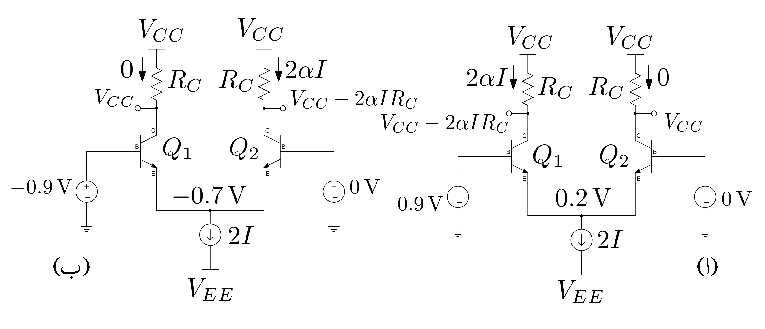
\includegraphics[scale=0.90]{differencePairWithDifferentialSignal}
\caption{ تفرقی اشارہ کے موجودگی میں تفرقی جوڑے کی کارکردگی}
\label{شکل_تفرقی_اشارے_کی_موجودگی_میں_تفرقی_جوڑے_کی_کارکردگی}
\end{figure}
تفرقی جوڑے کے دونوں دخول صفر وولٹ ہونے کی صورت میں \عددی{v_E=\SI{-0.7}{\volt}} ہوتا ہے۔اب اگر \عددی{v_{B2}=\SI{0}{\volt}} رکھتے ہوئے  \عددی{v_{B1}=\SI{-0.9}{\volt}} کر دیا جائے تو \عددی{Q_2} کا بیس-ایمٹر جوڑ سیدھا مائل ہو جائے گا لہٰذا \عددی{v_E=\SI{-0.7}{\volt}} ہو گا۔یوں \عددی{Q_1} کے بیس  سرے پر \عددی{\SI{-0.9}{\volt}} جبکہ اس کے ایمٹر سرے پر \عددی{\SI{-0.7}{\volt}} ہونے کی وجہ سے یہ منقطع صورت اختیار کر لے گا۔یہ صورت شکل \حوالہ{شکل_تفرقی_اشارے_کی_موجودگی_میں_تفرقی_جوڑے_کی_کارکردگی} ب میں دکھائی گئی ہے۔یوں منبع رو کی تمام برقی رو (یعنی \عددی{2 \times I} ) ٹرانزسٹر \عددی{Q_2} کو منتقل ہو جائے گی۔اس طرح
\begin{align*}
i_{E1}&=0\\
i_{E2}&=2 I\\
v_{C1}&=V_{CC}\\
v_{C2}&=V_{CC}-2 \alpha I R_C\\
v_o&=v_{C2}-v_{C1}=-2 \alpha I R_C
\end{align*}
ہوں گے۔شکل \حوالہ{شکل_تفرقی_اشارے_کی_موجودگی_میں_تفرقی_جوڑے_کی_کارکردگی} الف میں ہم نے دیکھا کہ \عددی{v_d=v_{B1}-v_{B2}=\SI{+0.9}{\volt}} کی صورت میں تفرقی جوڑا تمام کی تمام برقی رو (یعنی \عددی{2 \times I}) کو ایک ٹرانزسٹر میں منتقل کر چکا ہوتا ہے اور یوں یہ \عددی{v_o=+2 \alpha I R_C}  خارج کرتا ہے جبکہ شکل  ب میں \عددی{v_d=\SI{-0.9}{\volt}} ہیں اور تفرقی جوڑا تمام کی تمام برقی رو کو دوسرے ٹرانزسٹر میں منتقل کر کے \عددی{v_o=-2 \alpha I R_C}  خارج کرتا ہے۔

\حصہ{باریک داخلی تفرقی اشارہ پر تفرقی جوڑے کی بنیادی کارکردگی}
کرخوف کے قانون برائے برقی رو کے تحت \عددی{i_{E1}+i_{E2}=2 \times I} رہے گا۔اب تصور کریں کہ تفرقی جوڑے کو باریک تفرقی اشارہ \عددی{v_d} مہیا کیا جاتا ہے۔باریک تفرقی اشارہ سے مراد اتنی \عددی{v_d} ہے جس سے تمام کی تمام برقی رو \عددی{2 \times I}  کسی ایک ٹرانزسٹر میں منتقل نہ ہو۔ جیسا شکل \حوالہ{شکل_باریک_تفرقی_اشارے_پر_صورت_حال}  میں دکھایا گیا ہے، ہم اس صورت کو یوں بیان کر سکتے ہیں کہ  \عددی{+\frac{v_d}{2}}  اشارہ بطور \عددی{v_{B1}} اور  \عددی{-\frac{v_d}{2}} اشارہ بطور \عددی{v_{B2}} مہیا کیا جاتا ہے یعنی
\begin{align*}
v_{B1}&=+\frac{v_d}{2}\\
v_{B2}&=-\frac{v_d}{2}
\end{align*}
اگر  \عددی{v_{B1}} اور \عددی{v_{B2}} دونوں پر صفر وولٹ دئے جاتے تب \عددی{i_{E1}=i_{E2}=I} ہوتا۔اب جب \عددی{v_{B1}}  کو ہلکا بڑھایا اور \عددی{v_{B2}} کو گھٹایا  گیا ہے تو \عددی{i_{B1}}  میں \عددی{\Delta I}  کا اضافہ ہو گا جبکہ \عددی{i_{B2}}  میں اتنی ہم کمی واقع ہو گی۔ تا ہم اب بھی \عددی{i_{E1}+i_{E2}=2I} ہو گا۔یوں
\begin{figure}
\centering
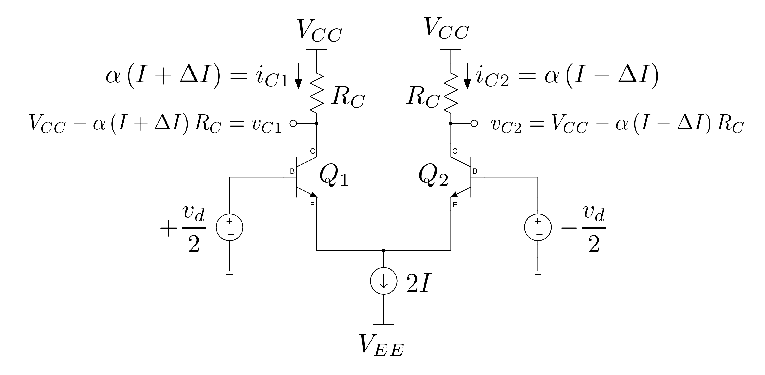
\includegraphics[scale=0.90]{differencePairWithSmallDifferentialSignal}
\caption{ باریک تفرقی اشارے پر صورت حال}
\label{شکل_باریک_تفرقی_اشارے_پر_صورت_حال}
\end{figure}
%
\begin{align*}
i_{E1}&=I+\Delta I\\
i_{E2}&=I-\Delta I
\end{align*}
ہوں  گے۔ لہٰذا
\begin{align*}
i_{C1}&=\alpha I_{E1}=\alpha \left(I+\Delta I \right )\\
i_{C2}&=\alpha I_{E2}=\alpha \left(I-\Delta I \right )\\
v_{C1}&=V_{CC}-i_{C1}R_C=V_{CC}-\alpha \left(I+\Delta I \right )R_C\\
v_{C2}&=V_{CC}-i_{C2}R_C=V_{CC}-\alpha \left(I-\Delta I \right )R_C\\
v_o&=v_{C2}-v_{C1}=+2 \alpha \Delta I R_C
\end{align*}
ہوں گے۔یہاں یہ بات ذہن نشین کرنا ضروری ہے کہ تفرقی جوڑے کے ایک ٹرانزسٹر کی برقی رو میں جتنا بھی اضافہ ( یا کمی ) پیدا ہو، دوسرے ٹرانزسٹر میں اتنی ہی کمی ( یا اضافہ ) پیدا ہوتا ہے۔

\حصہ{وسیع داخلی اشارہ پر تفرقی جوڑے کی کارکردگی}
اس حصہ میں تفرقی جوڑے پر تفصیلی غور کیا جائے گا۔ \عددی{Q_1} کے بیس  سرے پر \عددی{v_{B1}} جبکہ اس کے ایمٹر سرے پر \عددی{v_{E1}} برقی دباو پایا جاتا ہے۔چونکہ دونوں ٹرانزسٹر کے ایمٹر سرے آپس میں جڑے ہیں لہٰذا \عددی{v_{E1}=v_{E2}=v_E} ہو گا۔یوں ایمٹر سرے کے برقی دباو کو \عددی{v_{E1}} اور \عددی{v_{E2}} لکھنے کے بجائے \عددی{ v_E} لکھ سکتے ہیں۔اس طرح
\begin{align}
v_{BE1}=v_{B1}-v_{E1}=v_{B1}-v_E
\end{align}
ہو گا۔اسی طرح \عددی{Q_2} کے لئے ہم لکھ سکتے ہیں
\begin{align}
v_{BE2}=v_{B2}-v_{E2}=v_{B2}-v_E
\end{align}
ان برقی دباو کو استعمال کر کے ہم لکھ سکتے ہیں
\begin{align}
i_{C1}&=I_S \left(e^{\frac{v_{BE1}}{V_T}}-1 \right ) \approx I_S e^{\frac{v_{BE1}}{V_T}} =I_S e^{\frac{v_{B1}-v_E}{V_T}}\\
i_{C2}&=I_S \left(e^{\frac{v_{BE2}}{V_T}}-1 \right ) \approx I_S e^{\frac{v_{BE2}}{V_T}} =I_S e^{\frac{v_{B2}-v_E}{V_T}}
\end{align}
یوں
\begin{align}
i_{E1}&=\frac{i_{C1}}{\alpha}=\frac{I_S}{\alpha} e^{\frac{v_{B1}-v_E}{V_T}} \label{مساوات_تفرقی_پہلی_رو_بالمقابل_دباو}\\
i_{E2}&=\frac{i_{C2}}{\alpha}=\frac{I_S}{\alpha} e^{\frac{v_{B2}-v_E}{V_T}} \label{مساوات_تفرقی_دوسری_رو_بالمقابل_دباو}
\end{align}
ان مساوات میں \عددی{v_{B1}}  اور \عددی{v_{B2}} داخلی اشارات ہیں جنہیں آزاد متغیرات تصور کیا جائے  جبکہ \عددی{i_{E1}} اور \عددی{i_{E2}}  تابع متغیرات ہیں جن کا حصول درکار ہے۔آئیں انہیں حاصل کریں۔پہلے قدم میں مساوات \حوالہ{مساوات_تفرقی_دوسری_رو_بالمقابل_دباو}  کو مساوات \حوالہ{مساوات_تفرقی_پہلی_رو_بالمقابل_دباو}  سے تقسیم کر کے \عددی{v_E} سے چھٹکارا حاصل کیا جاتا ہے۔
\begin{align}
\frac{i_{E2}}{i_{E1}}=\frac{\left(\frac{I_S}{\alpha} e^{\frac{v_{B2}-v_E}{V_T}}\right )}{\left(\frac{I_S}{\alpha} e^{\frac{v_{B1}-v_E}{V_T}}\right )}=e^{\left(\frac{v_{B2}-v_{B1}}{V_T} \right )}=e^{-\frac{v_d}{V_T}}
\end{align}
جہاں \عددی{(v_{B1}-v_{B2})}  کو \عددی{v_d} لکھا گیا ہے۔دونوں جانب ایک   \عددی{(1)} جمع کرتے ہیں
\begin{align}
\frac{i_{E2}}{i_{E1}}+1&=1+ e^{\frac{v_d}{V_T}}\\
\frac{i_{E2}+i_{E1}}{i_{E1}}&=1+e^{-\frac{v_d}{V_T}}
\end{align}
چونکہ \عددی{i_{E1}+i_{E2}=2 \times I} ہوتا ہے لہٰذا اس مساوات کو یوں لکھ سکتے ہیں
\begin{align}
\frac{2 \times I}{i_{E1}}=1+e^{-\frac{v_d}{V_T}}
\end{align}
اسے الٹا کرنے سے تابع متغیرہ \عددی{i_{E1}}  حاصل ہوتا ہے
\begin{gather}
\begin{aligned}
\left( \frac{2 \times I}{i_{E1}}\right )^{-1}&=\left(1+e^{-\frac{v_d}{V_T}} \right )^{-1}\\
\frac{i_{E1}}{2 \times I}&=\frac{1}{\left(1+e^{-\frac{v_d}{V_T}} \right )}
\end{aligned}
\end{gather}
یعنی
\begin{align} \label{مساوات_تفرقی_پہلی_رو_بالمقابل_تفرقی_دباو}
i_{E1}=\frac{2 \times I}{\left(1+e^{-\frac{v_d}{V_T}} \right )}
\end{align}
اگر ہم مساوات \حوالہ{مساوات_تفرقی_پہلی_رو_بالمقابل_دباو}  کو مساوات \حوالہ{مساوات_تفرقی_دوسری_رو_بالمقابل_دباو}  سے تقسیم کرتے تو مندرجہ ذیل مساوات حاصل ہوتا۔
\begin{align} \label{مساوات_تفرقی_دوسری_رو_بالمقابل_تفرقی_دباو}
i_{E2}=\frac{2 \times I}{\left(1+e^{+\frac{v_d}{V_T}} \right )}
\end{align}
مساوات \حوالہ{مساوات_تفرقی_پہلی_رو_بالمقابل_تفرقی_دباو}  اور مساوات \حوالہ{مساوات_تفرقی_دوسری_رو_بالمقابل_تفرقی_دباو} شکل \حوالہ{شکل_تفرقی_جوڑے_کے_رو_بالمقابل_دباو_کے_خط}  میں کھینچے گئے ہیں۔
\begin{figure}
\centering
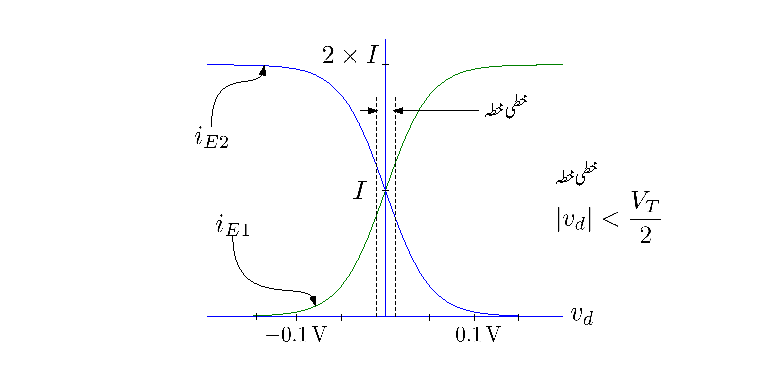
\includegraphics[scale=0.90]{differencePairCurrentVersusVoltage}
\caption{تفرقی جوڑے کے \عددی{v_d - i_d} خط}
\label{شکل_تفرقی_جوڑے_کے_رو_بالمقابل_دباو_کے_خط}
\end{figure}
%========
\ابتدا{مثال} \شناخت{مثال_تفرقی_صفر_دباو_پر_رو_کی_تقسیم}
صفر وولٹ تفرقی اشارہ یعنی \عددی{v_d=0} پر \عددی{i_{E1}} اور \عددی{i_{E2}} حاصل کریں۔

حل:	مساوات \حوالہ{مساوات_تفرقی_پہلی_رو_بالمقابل_تفرقی_دباو}  سے حاصل ہوتا ہے
\begin{align*}
i_{E1}=\frac{2 \times I}{1+e^{-\frac{0}{V_T}}}=\frac{2 \times I}{1+e^{0}}=\frac{2 \times I}{1+1}=I
\end{align*}
اسی طرح مساوات \حوالہ{مساوات_تفرقی_دوسری_رو_بالمقابل_تفرقی_دباو}  سے حاصل ہوتا ہے
\begin{align*}
i_{E2}=\frac{2 \times I}{1+e^{+\frac{0}{V_T}}}=\frac{2 \times I}{1+e^{0}}=\frac{2 \times I}{1+1}=I
\end{align*}
\انتہا{مثال}
%=========

\ابتدا{مثال} \شناخت{مثال_تفرقی_مختلف_تفرقی_دباو_پر_رو_کی_تقسیم}
مندرجہ ذیل تفرقی برقی اشارات پر \عددی{i_{E2}} حاصل کریں۔
\begin{enumerate}
\item
\begin{align*}
v_d=\SI{-0.15}{\volt}
\end{align*}
\item
\begin{align*}
v_d=\SI{-0.1}{\volt}
\end{align*}
\item
\begin{align*}
v_d=\SI{+0.1}{\volt}
\end{align*}
\item
\begin{align*}
v_d=\SI{+0.15}{\volt}
\end{align*}
\end{enumerate}

حل:	مساوات \حوالہ{مساوات_تفرقی_دوسری_رو_بالمقابل_تفرقی_دباو}  کے تحت
\begin{enumerate}
\item
\begin{align*}
i_{E2}=\frac{2 \times I}{1+e^{\frac{-0.15}{0.025}}}=\frac{2 \times I}{1+0.0024788} \approx 2 \times I
\end{align*}
\item
\begin{align*}
i_{E2}=\frac{2 \times I}{1+e^{\frac{-0.1}{0.025}}}=\frac{2 \times I}{1+0.018316} = 0.982 \times  2 \times I
\end{align*}
\item
\begin{align*}
i_{E2}=\frac{2 \times I}{1+e^{\frac{+0.1}{0.025}}}=\frac{2 \times I}{1+54.598} =0.018 \times  2 \times I
\end{align*}
\item
\begin{align*}
i_{E2}=\frac{2 \times I}{1+e^{\frac{+0.15}{0.025}}}=\frac{2 \times I}{1+403.41} =0.00247 \times  2 \times I \approx 0
\end{align*}
\end{enumerate}

\انتہا{مثال}
%=========
مثال \حوالہ{مثال_تفرقی_صفر_دباو_پر_رو_کی_تقسیم}  سے صاف ظاہر ہے کہ تفرقی اشارہ کے عدم موجودگی میں دونوں ٹرانزسٹر میں برابر برقی رو پائی جاتی ہے۔مزید یہ کہ ان برقی رو پر \اصطلاح {مشترکہ اشارہ} \عددی{v_{CM}} کا کسی قسم کا کوئی اثر نہیں۔

مثال \حوالہ{مثال_تفرقی_مختلف_تفرقی_دباو_پر_رو_کی_تقسیم}  میں \عددی{v_d=\SI{-0.1}{\volt}} پر \عددی{\num{98.2}} فی صد برقی رو  \عددی{Q_2}  سے گزرتی ہے جبکہ \عددی{v_d=\SI{+0.1}{\volt}} پر صرف \عددی{\num{1.8}}  فی صد اس میں سے گزرتی ہے۔اس سے یہ بات واضح ہوتی ہے کہ تفرقی اشارہ میں باریک تبدیلی سے تفرقی جوڑے میں برقی رو کی تقسیم بہت زیادہ متاثر ہوتی ہے۔

تفرقی جوڑے میں برقی رو کو ایک ٹرانزسٹر سے دوسرے ٹرانزسٹر میں منتقل کرنے کی خاطر نہایت کم داخلی تفرقی برقی دباو درکار ہوتا ہے۔مزید یہ کہ اس تمام عمل میں تفرقی جوڑے کے دونوں ٹرانزسٹر افزائندہ حال رہتے ہیں۔

جیسا کہ آپ جانتے ہیں کہ ٹرانزسٹر کے بیس-ایمٹر جوڑ پر اندرونی کپیسٹر \عددی{C_{b'e}}  اور بیس-کلکٹر  جوڑ پر اندرونی کپیسٹر \عددی{C_{b'c}}  پائے جاتے ہیں۔غیر-افزائندہ ٹرانزسٹر میں ان کپیسٹروں کے مجموعہ کی قیمت، افزائندہ ٹرانزسٹر کے نسبت، زیادہ ہوتی ہے۔ان کپیسٹروں میں بار بھرنا یا ان سے بار کے نکاسی کے لئے وقت درکار ہوتا ہے۔اس درکار وقت کا دارومدار کل کپیسٹر کی قیمت اور ان دو مختلف برقی دباو (جن کے مابین اس میں بار بھرا جائے یا بار کی نکاسی کی جائے) پر ہوتا ہے۔

تفرقی جوڑا چونکہ ہر صورت افزائندہ رہتا ہے لہٰذا اس کے کپیسٹر کی قیمت کم ترین رہتی ہے اور چونکہ اسے چلانے کی خاطر درکار تفرقی اشارہ \عددی{v_d}  کے دو حدود  قریب قریب ہیں لہٰذا اسے استعمال کرتے ہوئے نہایت تیز رفتار ادوار تخلیق دینا ممکن ہوتا ہے۔یہی وجہ ہے کہ تیز ترین عددی برقیات (مثلاً \اصطلاح {ایمٹر جڑا منطق}\فرہنگ{ایمٹر جڑا منطق}\فرہنگ{emitter coupled logic}\حاشیہب{emitter coupled logic} ) میں بالخصوص اور دیگر تیز ترین برقیات میں بالعموم تفرقی جوڑا ہی استعمال ہوتا ہے۔



اس حصہ میں ہم تفرقی جوڑے کو بطور ایمپلیفائر استعمال کریں گے۔شکل \حوالہ{شکل_تفرقی_جوڑے_کے_رو_بالمقابل_دباو_کے_خط}  کو دیکھتے ہوئے معلوم ہوتا ہے کہ دو نقطہ دار لکیروں کے درمیان داخلی اشارہ \عددی{v_d} اور برقی رو  \عددی{i_{E1}} (یا \عددی{i_{E2}}) کے مابین خطی تعلق پایا جاتا ہے یعنی اس خطے میں \عددی{v_d} جتنے گنا بڑھایا یا گھٹایا جائے \عددی{i_{E1}} (یا \عددی{i_{E2}} ) میں اتنے گنا کی ہی تبدیلی پیدا ہوتی ہے۔خطی تعلق کا خطہ تقریباً
\begin{align}
\abs{v_d} < \frac{V_T}{2}
\end{align}
پر پایا جاتا ہے۔آئیں اس خطی خطے پر مزید غور کریں۔

\حصہ{باریک اشارہ پر تفرقی جوڑے کے کارکردگی پر تفصیلی غور}
\جزوحصہ{باریک اشاراتی مساوات}
مساوات \حوالہ{مساوات_تفرقی_پہلی_رو_بالمقابل_تفرقی_دباو}  اور مساوات \حوالہ{مساوات_تفرقی_دوسری_رو_بالمقابل_تفرقی_دباو}  قطعی مساوات ہیں جن سے تفرقی جوڑے میں برقی رو کی تقسیم حاصل کی جا سکتی ہے۔اگر ہم شکل \حوالہ{شکل_تفرقی_جوڑے_کے_رو_بالمقابل_دباو_کے_خط} میں دکھائے خطی خطے کی بات کریں تو اس خطے میں برقی رو کی تقسیم کو نہایت سادہ اور خطی مساوات سے بھی حاصل کیا جا سکتا ہے۔اس حصہ میں ان مساوات کو حاصل کرتے ہیں۔

مساوات \حوالہ{مساوات_تفرقی_پہلی_رو_بالمقابل_تفرقی_دباو}  کو یہاں دوبارہ پیش کرتے ہیں۔
\begin{align}\label{مساوات_تفرقی_جوڑا_برقی_رو_کی_اصل_مساوات}
i_{E1}=\frac{2 \times I}{1+e^{-\frac{v_d}{V_T}}}
\end{align}
اس مساوات کو \عددی{e^{\frac{1}{2}\frac{v_d}{V_T}}} سے ضرب اور تقسیم کرتے ہیں۔
\begin{align} \label{مساوات_تفرقی_پہلی_رو_بالمقابل_تفرقی_دباو_الف}
i_{E1}=\left( \frac{2 I}{1+e^{-\frac{v_d}{V_T}}}\right ) \left(\frac{e^{\frac{1}{2}\frac{v_d}{V_T}}}{e^{\frac{1}{2}\frac{v_d}{V_T}}} \right )=\frac{2I e^{\frac{1}{2}\frac{v_d}{V_T}}}{e^{+\frac{1}{2}\frac{v_d}{V_T}}+e^{-\frac{1}{2}\frac{v_d}{V_T}}}
\end{align}
آپ جانتے ہیں کہ باریک \عددی{x}  کی صورت میں \عددی{e^{+x}} اور \عددی{e^{-x}} کے  \اصطلاح {مکلارن تسلسل}\فرہنگ{مکلارن تسلسل}\فرہنگ{سلسلہ!مکلارن}\حاشیہب{Maclaurin series} یوں لکھے جا سکتے ہیں۔
\begin{align*}
e^{+x}&=1+x+\frac{x^2}{2!}+\frac{x^3}{3!}+\cdots\\
e^{-x}&=1-x+\frac{x^2}{2!}-\frac{x^3}{3!}+\cdots\\
\end{align*}
چونکہ خطی خطے میں \عددی{\abs{v_d} < \frac{V_T}{2}} ہے لہٰذا  \عددی{e^{+\frac{v_d}{V_T}}}  اور \عددی{e^{-\frac{v_d}{V_T}}} کے مکلارن تسلسل میں پہلے چند جزو کو چھوڑ کر بقایا تمام اجزاء کے  قیمتیں نہایت کم ہوں گی۔مساوات \حوالہ{مساوات_تفرقی_پہلی_رو_بالمقابل_تفرقی_دباو_الف}  میں \عددی{e^{+\frac{v_d}{V_T}}}  اور \عددی{e^{-\frac{v_d}{V_T}}}  کے  مکلارن تسلسل پُر کرتے ہیں۔
\begin{gather}
\begin{aligned}
i_{E1}&=2I \frac{1+\frac{1}{2}\frac{v_d}{V_T} \cdots}{\left( 1+\frac{1}{2}\frac{v_d}{V_T} \cdots\right )+\left(1-\frac{1}{2}\frac{v_d}{V_T}\cdots \right )}\\
& \approx 2I \frac{\left(1+\frac{1}{2}\frac{v_d}{V_T} \cdots \right )}{2}\\
& = I \left(1+\frac{1}{2} \frac{v_d}{V_T} \right )\\
&=I+\frac{I}{2}\frac{v_d}{V_T}
\end{aligned}
\end{gather}
جہاں دوسرے قدم پر تسلسل کے صرف پہلے دو جزو رکھے گئے۔یہ وہ سادہ خطی مساوات ہے جس کی تلاش تھی۔اس کو یوں لکھتے ہیں۔
\begin{align}
i_{E1}=I+\frac{I}{V_T}\frac{v_d}{2}
\end{align}
اسی طرح اگر \عددی{i_{E2}} کی سادہ خطی مساوات حاصل کی جائے تو وہ مندرجہ ذیل ہو گی۔
\begin{align}\label{مساوات_تفرقی_جوڑا_دوسری_برقی_رو}
i_{E2}=I-\frac{I}{V_T}\frac{v_d}{2}
\end{align}
ان نتائج سے حاصل ہوتا ہے
\begin{gather}
\begin{aligned} \label{مساوات_تفرقی_پہلی_رو_تسلسل_کے_دو_جز}
i_{C1}&=\alpha i_{E1}=\alpha I +\frac{\alpha I}{V_T} \frac{v_d}{2}\\
i_{C2}&=\alpha i_{E2}=\alpha I -\frac{\alpha I}{V_T} \frac{v_d}{2}
\end{aligned}
\end{gather}
تفرقی اشارہ کے عدم موجودگی، یعنی \عددی{v_d=0} ، کی صورت میں \عددی{i_{E1}=i_{E2}=I}  ہی حاصل ہوتے ہیں جو کہ ان ٹرانزسٹر کے نقطہ کارکردگی پر برقی رو \عددی{I_{EQ1}} اور \عددی{I_{EQ2}}  ہیں۔اسی طرح \عددی{v_d=0} کی صورت میں مساوات \حوالہ{مساوات_تفرقی_پہلی_رو_تسلسل_کے_دو_جز}  سے \عددی{i_{C1}=\alpha I} اور \عددی{i_{C2}=\alpha I} حاصل ہوتا ہے جو نقطہ کارکردگی پر کلکٹر برقی رو ہیں جنہیں \عددی{I_{CQ}} یا صرف \عددی{I_{C}} لکھا جا سکتا ہے۔تفرقی اشارہ کے موجودگی میں مساوات \حوالہ{مساوات_تفرقی_پہلی_رو_تسلسل_کے_دو_جز} میں یک سمت رو کے علاوہ بدلتا رو بھی پائی جاتی ہے۔یوں انہیں
\begin{gather}
\begin{aligned}
i_{C1}&=ِI_{C}+\frac{\alpha I}{V_T} \frac{v_d}{2}\\
&=I_{C}+i_c\\
i_{C2}&=ِI_{C}-\frac{\alpha I}{V_T} \frac{v_d}{2}\\
&=I_{C}-i_c
\end{aligned}
\end{gather}
لکھا جا سکتا ہے جہاں  \عددی{i_c} بدلتا برقی رو یعنی
\begin{align}
i_c=\frac{\alpha I}{V_T}\frac{v_d}{2}=\left(\frac{I_{C}}{V_T}\right) \frac{v_d}{2}
\end{align}
ہے۔آپ صفحہ \حوالہصفحہ{مساوات_ٹرانزسٹر_افزائش_موصلیت_نما} پر دئے گئے مساوات \حوالہ{مساوات_ٹرانزسٹر_افزائش_موصلیت_نما} کی مدد سے جانتے ہیں کہ \عددی{\frac{I_C}{V_T}} دراصل \عددی{g_m} ہے لہٰذا اسے مزید اس طرح لکھ سکتے ہیں۔

\begin{align} \label{مساوات_تفرقی_اشاراتی_رو}
i_c=g_m \frac{v_d}{2}
\end{align}
اس طرح مساوات \حوالہ{مساوات_تفرقی_پہلی_رو_تسلسل_کے_دو_جز} کو یوں لکھ سکتے ہیں۔
\begin{gather}
\begin{aligned}
i_{C1}&=I_{C}+g_m \frac{v_d}{2}\\
i_{C2}&=I_{C} - g_m \frac{v_d}{2}
\end{aligned}
\end{gather}
یہاں رک کر شکل \حوالہ{شکل_باریک_تفرقی_اشارے_پر_صورت_حال}  میں دکھائے \عددی{i_{C1}} اور \عددی{i_{C2}} کا مساوات \حوالہ{مساوات_تفرقی_پہلی_رو_تسلسل_کے_دو_جز} میں حاصل کئے گئے قیمتوں کے ساتھ موازنہ کریں۔آپ دیکھ سکتے ہیں کہ  \عددی{\alpha \Delta I = \frac{\alpha I}{V_T}\frac{v_d}{2}}ہے۔باریک داخلی اشارے پر  مساوات \حوالہ{مساوات_تفرقی_اشاراتی_رو}  کی مدد سے  تفرقی جوڑے میں برقی رو \عددی{i_c}  حاصل کی جا سکتی ہے۔یہ ایک اہم نتیجہ ہے جس پر اگلے حصے میں تبصرہ کیا جائے گا۔


\جزوحصہ{برقی رو کا حصول بذریعہ ٹرانزسٹر ریاضی نمونہ}
 گزشتہ حصہ میں مساوات \حوالہ{مساوات_تفرقی_اشاراتی_رو}  حاصل کی گئی جس کے مدد سے تفرقی جوڑے میں برقی رو  \عددی{i_c}  حاصل کی جا سکتی ہے۔آئیں اسی مساوات کو انتہائی سادہ طریقہ سے  حاصل کریں۔
\begin{figure}
\centering
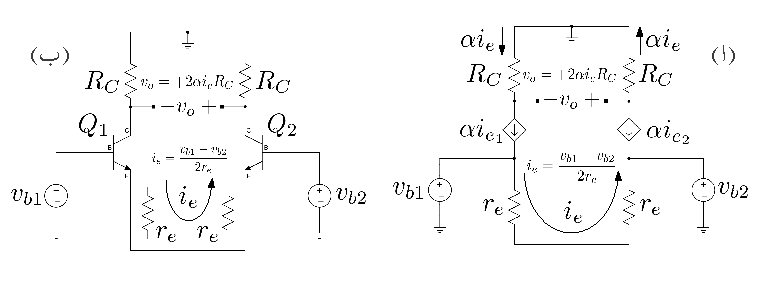
\includegraphics[scale=0.90]{differencePairUsingModel}
\caption{تفرقی برقی رو کا حصول بذریعہ ریاضی نمونہ}
\label{شکل_تفرقی_رو_بذریعہ_ماڈل}
\end{figure}
شکل \حوالہ{شکل_تفرقی_رو_بذریعہ_ماڈل} ب میں تفرقی جوڑے کا مساوی بدلتا رو شکل دکھایا گیا ہے جہاں تمام یک سمت منبع برقی دباو کو قصر دور  اور تمام یک سمت منبع برقی رو کو کھلے سرے  کیا گیا ہے۔شکل \حوالہ{شکل_تفرقی_رو_بذریعہ_ماڈل} الف میں ٹرانزسٹر کے ٹی-ریاضی نمونہ استعمال کر کے اسی کا مساوی دور بنایا گیا ہے جہاں سے صاف ظاہر ہے کہ
\begin{align}
i_e=\frac{v_{b1}-v_{b2}}{2 r_e}=\frac{v_d}{2 r_e}
\end{align}
ہو گا جہاں \عددی{v_{b1}-v_{b2}}  کو \عددی{v_d} لکھا گیا ہے۔یوں \عددی{i_{e_1}=i_e} جبکہ \عددی{i_{e2}=-i_e} کے برابر ہو گا۔صفحہ \حوالہصفحہ{مساوات_ٹرانزسٹر_اندرونی_مخارج_مزاحمت_کی_مساوات} پر مساوات \حوالہ{مساوات_ٹرانزسٹر_اندرونی_مخارج_مزاحمت_کی_مساوات} کے تحت \عددی{r_e=\frac{\alpha}{g_m}} کے برابر ہے۔یوں اس مساوات کو اس طرح لکھ سکتے ہیں۔
\begin{align}
i_e=\frac{g_m}{\alpha} \frac{v_d}{2}
\end{align}
اور یوں
\begin{align}
i_c = \alpha i_e = g_m \frac{v_d}{2}
\end{align}
اس طرح نہایت آسانی سے اس مساوات کو حاصل کیا گیا۔

یہ مساوات حاصل کرتے وقت ریاضی نمونہ بنانا ضروری نہیں۔ شکل \حوالہ{شکل_تفرقی_رو_بذریعہ_ماڈل} ب میں ایمٹر سرے کے مزاحمت \عددی{r_e} کو تفرقی جوڑے کے اندر جانب دکھایا گیا ہے۔یہ ایک تصوراتی شکل ہے جسے دیکھ کر آپ مساوت  لکھ سکتے ہیں۔

ان دونوں اشکال کو دیکھ کر خارجی برقی دباو \عددی{v_o}حاصل کیا جا سکتا ہے یعنی
\begin{align}
v_o=+i_c \times 2 \times R_C=+g_m R_C v_d
\end{align}
اس مساوات سے \اصطلاح {تفرقی افزائش برقی دباو}\فرہنگ{تفرقی!افزائش}\حاشیہب{differential voltage gain}  \عددی{A_d=\frac{v_o}{v_d}} حاصل کی جا سکتی ہے۔
\begin{align}
A_d=\frac{v_o}{v_d}=+g_m R_C
\end{align}
%
\begin{figure}
\centering
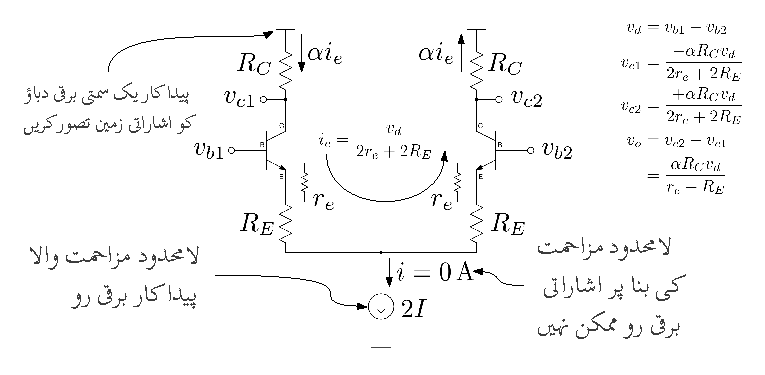
\includegraphics[scale=0.90]{differencePairExampleA}
\caption{ اشاراتی برقی رو کے سادہ طریقہ کی ایک اور مثال}
\label{شکل_اشاراتی_برقی_رو_کے_سادہ_طریقے_کی_ایک_اور_مثال}
\end{figure}
موجودہ طریقے کی افادیت دیکھنے کی خاطر شکل \حوالہ{شکل_اشاراتی_برقی_رو_کے_سادہ_طریقے_کی_ایک_اور_مثال}  میں دکھائے تفرقی ایمپلیفائر پر غور کریں جہاں ٹرانزسٹر کے ایمٹر سرے پر بیرونی مزاحمت \عددی{R_E} نسب کئے گئے ہیں۔اس دور کو دیکھ کر ہی ہم لکھ سکتے ہیں۔
\begin{align*}
i_e=\frac{v_d}{2 r_e +2 R_E}
\end{align*}
اس مساوات سے \اصطلاح {تفرقی افزائش برقی دباو} حاصل ہوتی ہے۔
\begin{gather}
\begin{aligned}
i_c&= \alpha i_e =\frac{\alpha v_d}{2 r_e + 2 R_E}\\
v_o&=+2 i_c R_C=+\frac{\alpha v_d R_C}{r_e+ R_E}\\
A_d&=\frac{v_o}{v_d}=+\frac{\alpha R_C}{r_e+R_E} \approx +\frac{R_C}{r_e+R_E}
\end{aligned}
\end{gather}
یاد رہے کہ اشاراتی تجزیہ کرتے وقت یک سمت برقی دباو کو قصر دور جبکہ یک سمت برقی رو کو آزاد  سرے کر دیا جاتا ہے۔ 



\جزوحصہ{داخلی تفرقی مزاحمت}
\begin{figure}
\centering
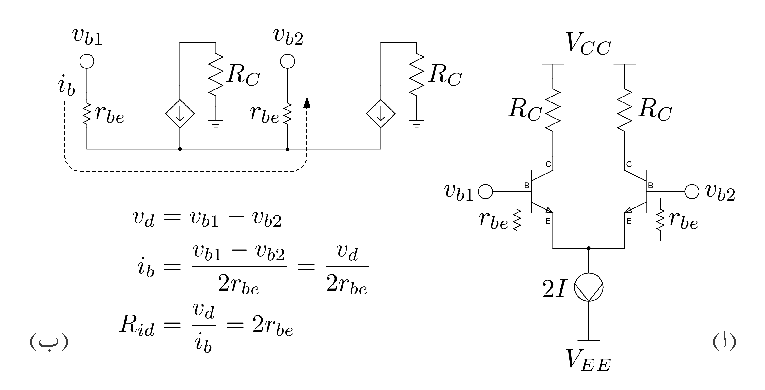
\includegraphics[scale=0.90]{differencePairInputResistance}
\caption{تفرقی جوڑے کی داخلی تفرقی مزاحمت}
\label{شکل_تفرقی_جوڑے_کی_داخلی_مزاحمت}
\end{figure}
تفرقی جوڑے میں دونوں ٹرانزسٹر کے \عددی{\pi}  ریاضی نمونہ استعمال کرتے شکل \حوالہ{شکل_تفرقی_جوڑے_کی_داخلی_مزاحمت} ب حاصل ہوتا ہے جس سے اس کی داخلی برقی رو \عددی{i_b} 
\begin{align}
i_b=\frac{v_{b1}-v_{b2}}{2 r_{be}}=\frac{v_d}{2 r_{be}}
\end{align}
اور اس سے تفرقی جوڑے کا \اصطلاح {داخلی تفرقی مزاحمت}\فرہنگ{داخلی!تفرقی مزاحمت}\فرہنگ{مزاحمت!تفرقی داخلی}\فرہنگ{differential input resistance}\حاشیہب{differential input resistance}  یوں حاصل ہوتا ہے۔
\begin{align}
R_{id}=\frac{v_b}{i_b}=2 r_{be}
\end{align}
یہی دو جوابات مکمل ریاضی نمونہ بنانے کے بغیر بھی حاصل کئے جا سکتے ہیں جیسے شکل \حوالہ{شکل_تفرقی_جوڑے_کی_داخلی_مزاحمت} الف میں دکھایا گیا ہے جہاں دونوں ٹرانزسٹر کے داخلی مزاحمت \عددی{r_{be}}  کو  ان کے داخلی جانب دکھا کر واضح کیا گیا ہے۔

اسی طریقے کو شکل \حوالہ{شکل_اشاراتی_برقی_رو_کے_سادہ_طریقے_کی_ایک_اور_مثال}  میں دکھائے تفرقی جوڑے کے لئے استعمال کرتے ہیں۔چونکہ اس شکل میں
\begin{align}
i_e=\frac{v_d}{2 r_e+2 R_E}
\end{align}
ہے لہٰذا
\begin{align}
i_b=\frac{i_e}{\beta+1}=\frac{1}{\beta+1} \left(\frac{v_d}{2 r_e +2 R_E} \right )
\end{align}
ہو گا جس سے \اصطلاح {داخلی تفرقی مزاحمت} یوں حاصل ہوتا ہے۔
\begin{align}
R_{id}=\frac{v_d}{i_b}=\left(\beta+1 \right ) \left(2 r_e+2 R_E \right )
\end{align}
اب تک ہم تصور کرتے رہے ہیں کہ تفرقی ایمپلیفائر میں استعمال کئے جانے والے یک سمت  منبع رو کی اندرونی مزاحمت لامحدود ہوتی ہے۔حقیقت میں پائے جانے والے یک سمت  منبع رو کی اندرونی مزاحمت نہایت زیادہ مگر محدود ہوتی ہے۔شکل \حوالہ{شکل_باریک_اشاراتی_مزاحمت_کو_زیر_نظر} الف میں یک سمت  منبع رو کا مساوی \اصطلاح {نارٹن دور}\حاشیہب{Norton equivalent} استعمال کرتے ہوئے اس کے اندرونی باریک اشاراتی مزاحمت  \عددی{R} کو بھی شامل کیا گیا ہے۔اس شکل میں ٹرانزسٹر کا اندرونی مزاحمت  \عددی{r_e} کو تفرقی جوڑے کے اندر جانب فرضی طور دکھایا گیا ہے۔شکل \حوالہ{شکل_باریک_اشاراتی_مزاحمت_کو_زیر_نظر} ب میں اس ایمپلیفائر کے داخلی جانب کا باریک اشاراتی ریاضی نمونہ دکھایا گیا ہے۔
\begin{figure}
\centering
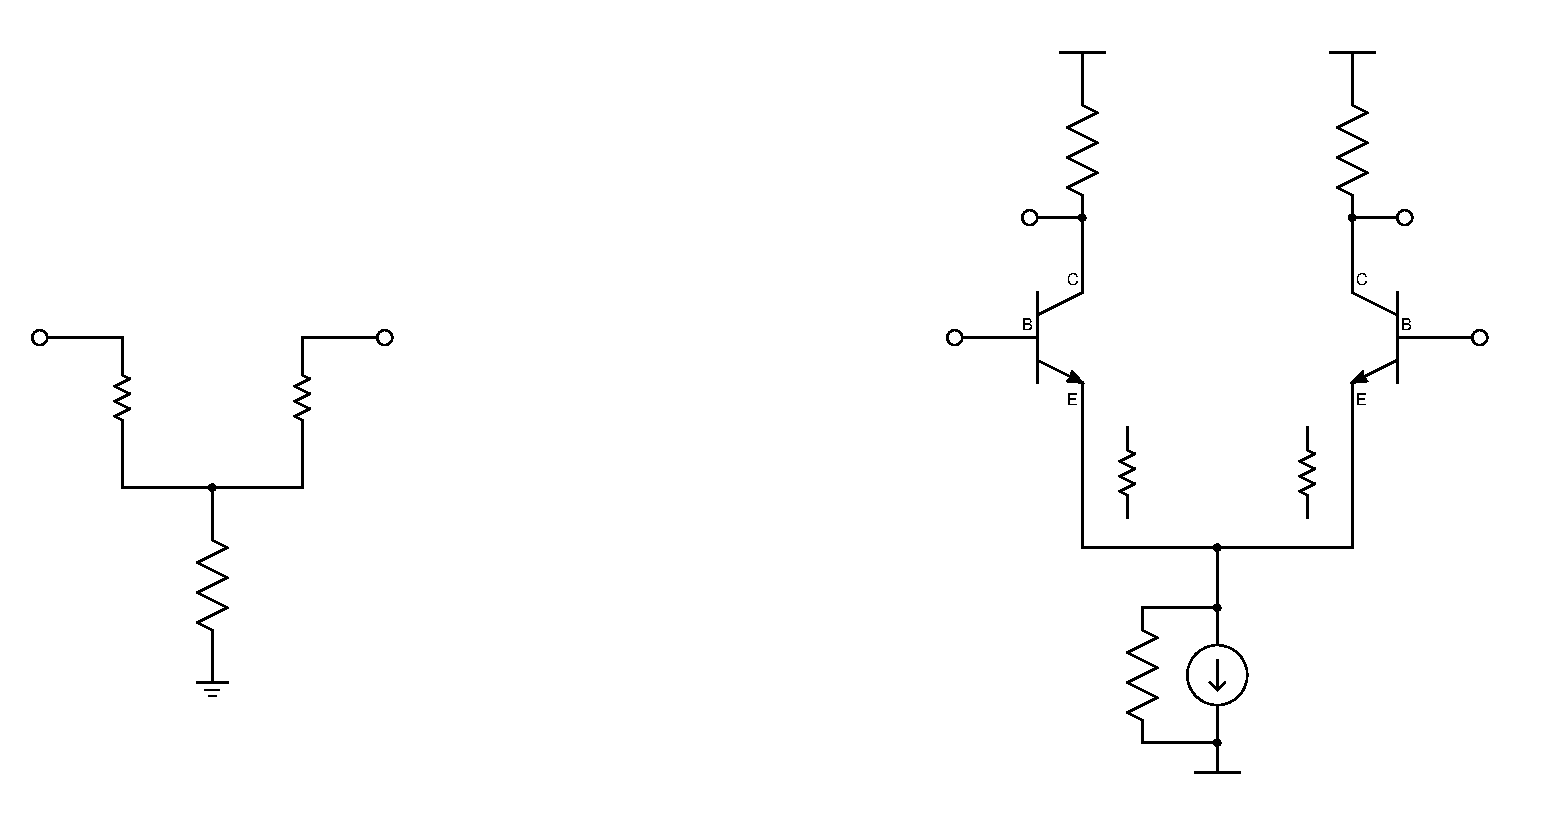
\includegraphics[scale=0.90]{differencePairInputResistanceA}
\caption{باریک اشاراتی مزاحمت کو زیرِ نظر رکھتے ہوئے داخلی تفرقی مزاحمت}
\label{شکل_باریک_اشاراتی_مزاحمت_کو_زیر_نظر}
\end{figure}
ٹرانزسٹروں کے ایمٹر سرے کا برقی دباو \عددی{v_e} حاصل کرنے کی خاطر اس جوڑ پر کرخوف کا قانون برائے برقی رو نافذ کرتے ہیں۔
\begin{align}
\frac{v_e - \frac{v_d}{2}}{r_e} + \frac{v_e + \frac{v_d}{2}}{r_e} +\frac{v_e}{R}=0
\end{align}
اس مساوات سے حاصل ہوتا ہے۔
\begin{align}\label{مساوات_تفرقی_جوڑا_تفرقی_اشارے_کے_لئے_جوڑے_کی_مخارج_برقی_زمین_ہے}
v_e=0
\end{align}
اس نتیجے کے مطابق باریک تفرقی اشارہ \عددی{v_d}  کا \عددی{v_e} پر کوئی اثر نہیں ہوتا اور \عددی{v_e}   ہر وقت صفر وولٹ یعنی برقی زمین پر رہتا ہے۔اس حقیقت کو مدِ نظر رکھتے ہوئے شکل \حوالہ{شکل_باریک_اشاراتی_مزاحمت_کو_زیر_نظر} الف  کا (باریک تفرقی اشارہ کے لئے) مساوی سادہ دور شکل \حوالہ{شکل_تفرقی_جوڑا_بطور_مخارج_جڑے_ایمپلیفائر} الف میں دکھایا گیا ہے۔اس شکل میں تفرقی ایمپلیفائر کو دو عدد \اصطلاح {مشترک-ایمٹر ایمپلیفائر}\فرہنگ{مشترک-مخارج}\فرہنگ{CE amplifier}  تصور کرنا دکھایا گیا ہے جہاں بائیں ہاتھ کے ایمپلیفائر کا داخلی اشارہ \عددی{+\frac{v_d}{2}} اور اس کا خارجی اشارہ \عددی{v_{c1}} ہے جبکہ دائیں ایمپلیفائر کا داخلی اشارہ \عددی{-\frac{v_d}{2}} اور اس کا خارجی اشارہ \عددی{v_{c2}} ہے۔شکل  ب میں بائیں ہاتھ کے ایمپلیفائر کا باریک اشاراتی ریاضی نمونہ دکھایا گیا ہے جہاں ٹرانزسٹر کے اندرونی \اصطلاح {خارجی مزاحمت} \عددی{r_o} کے اثر کو بھی شامل کیا گیا ہے۔اس  ریاضی نمونہ سے آدھے دور کا \اصطلاح {داخلی باریک اشاراتی مزاحمت} \عددی{r_{be}}  کے برابر حاصل ہوتا ہے۔تفرقی ایمپلیفائر کا داخلی باریک اشاراتی مزاحمت اس کا دگنا ہو گا یعنی
\begin{align}
R_{id}=2 r_{be}
\end{align}
اگر \عددی{v_o}  کو \عددی{v_{c1}} اور \عددی{v_{c2}} کے مابین لیا جائے تب تفرقی افزائش برقی دباو
\begin{align}
A_d=\frac{v_o}{v_d}=\frac{v_{c2}-v_{c1}}{v_d}=g_m \left(R_C  \parallel r_o \right )
\end{align}
حاصل ہوتا ہے۔عموماً \عددی{r_o} کی قیمت  \عددی{R_C} کے قیمت سے بہت زیادہ ہوتی ہے اور یوں اس مساوات کو یوں لکھا جا سکتا ہے۔
\begin{align} \label{مساوات_تفرقی_پوری_تفرقی_افزائش}
A_{\textup{dپوری}}=\frac{v_{c2}-v_{c1}}{v_d}=g_m R_C=\frac{R_C}{r_e}
\end{align}
اس کے برعکس اگر \عددی{v_o} کو \عددی{v_{c1}}  (یا \عددی{v_{c2}} ) سے حاصل کیا جائے تب تفرقی افزائش برقی دباو یوں حاصل ہوتی ہے۔
\begin{align} \label{مساوات_تفرقی_آدھی_تفرقی_افزائش}
A_{\textup{dآدھی}}=\frac{v_o}{v_d}=\frac{v_{c1}}{v_d}=-\frac{R_C}{2 r_e}
\end{align}
%
\begin{figure}
\centering
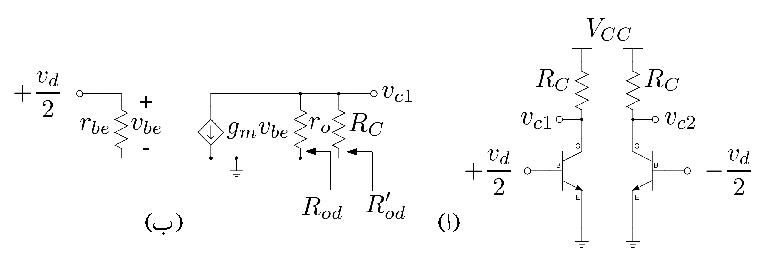
\includegraphics[scale=0.90]{differencePairAsTwoEmitterConnectedAmplifiers}
\caption{تفرقی ایمپلیفائر بطور دو عدد ایمٹر جڑے ایمپلیفائر}
\label{شکل_تفرقی_جوڑا_بطور_مخارج_جڑے_ایمپلیفائر}
\end{figure}
شکل \حوالہ{شکل_تفرقی_جوڑا_بطور_مخارج_جڑے_ایمپلیفائر} ب میں آدھے ایمپلیفائر کے خارجی تفرقی مزاحمت \عددی{R_{od}} اور \عددی{R_{od}'}  دکھائے گئے ہیں۔ \عددی{R_{od}} وہ مزاحمت ہے جس میں  \عددی{R_C} کے اثر کو شامل نہیں کیا گیا یعنی اس میں \عددی{R_C} کو لامحدود تصور کرتے دور کا مزاحمت حاصل کیا گیا ہے۔ہم کہتے ہیں کہ یہ مزاحمت \عددی{R_C}  سے پہلا کا مزاحمت ہے۔ \عددی{R_{od}} کی قیمت \عددی{r_o} ہے۔ \عددی{R_{od}'} آدھے ایمپلیفائر کا وہ خارجی تفرقی مزاحمت ہے جو ٹرانزسٹر کے اندرونی مزاحمت \عددی{r_o}  اور اس کے ساتھ منسلک بیرونی مزاحمت \عددی{R_C} دونوں کے اثر کو شامل کرتا ہے۔اس کی قیمت \عددی{(r_o \parallel R_C)} ہے۔


\جزوحصہ{داخلی مشترکہ مزاحمت اور مشترکہ افزائش}
شکل \حوالہ{شکل_مشترکہ_آدھے_دور_کا_حصول} الف میں تفرقی جوڑے کو مشترکہ داخلی اشارہ \عددی{v_{CM}}  فراہم کیا گیا ہے۔دونوں ہاتھوں کے ٹرانزسٹروں میں یکساں برقی رو \عددی{i_e} گزرے گی اور یوں
\begin{align}
v_e=\left(i_{e1}+i_{e2} \right ) R=2 i_e R
\end{align}
ہو گا۔اسی کو شکل  ب کے طرز پر بھی بنایا جا سکتا ہے۔آپ دیکھ سکتے ہیں کہ اب بھی \عددی{v_e} کی قیمت وہی ہے یعنی
\begin{align}
v_e=i_e (2 R)=2 i_e R
\end{align}
اسی طرح دونوں اشکال میں ٹرانزسٹروں میں یک سمت برقی رو کی قیمت \عددی{I} ہی ہے۔یوں مشترکہ اشارے کے لئے شکل  الف کو دو یکساں ایمپلیفائر تصور کیا جا سکتا ہے۔شکل  ب سے
\begin{align}
i_e=\frac{v_{CM}}{r_e+ 2R}
\end{align}
حاصل ہوتا ہے جس سے ایک بازو کا مشترکہ مزاحمت یوں حاصل ہوتا ہے
\begin{gather}
\begin{aligned}
i_b&=\frac{i_e}{\beta+1}=\frac{v_{CM}}{\left(\beta+1 \right )\left( r_e + 2 R\right )}\\
R_{\textup{icmآدھا}}&=\frac{v_{CM}}{i_b}=\left(\beta+1 \right ) \left( r_e + 2 R\right )
\end{aligned}
\end{gather}
تفرقی ایمپلیفائر کا مشترکہ داخلی مزاحمت اس کے دگنا ہو گا یعنی
\begin{align}
R_{icm}=2 \left (\beta+1 \right ) \left(r_e + 2 R \right )
\end{align}
مزید یہ کہ 
\begin{align}
v_{c1}=v_{c2}=-\alpha i_e R_C = -\frac{\alpha R_C v_{CM}}{r_e+ 2 R}
\end{align}
%
\begin{figure}
\centering
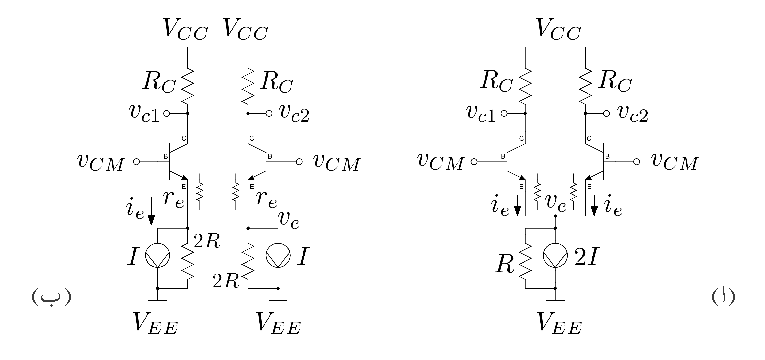
\includegraphics[scale=0.90]{commonModeHalfCircuit}
\caption{مشترکہ آدھے دور کا حصول}
\label{شکل_مشترکہ_آدھے_دور_کا_حصول}
\end{figure}
حاصل ہوتے ہیں۔ اگر خارجی اشارہ \عددی{v_o}  کو \عددی{v_{c1}} اور \عددی{v_{c2}} کے مابین لیا جائے تب اس کی قیمت صفر وولٹ ہو گی اور \اصطلاح {مشترکہ افزائش برقی دباو}\فرہنگ{مشترکہ افزائش}\حاشیہب{common mode voltage gain}\فرہنگ{common mode voltage gain} صفر ہو گا۔البتہ اگر \عددی{v_o} کو \عددی{v_{c1}}   ( یا \عددی{v_{c2}} ) سے حاصل کیا جائے تب
\begin{align}
v_o=v_{c1}=-\frac{\alpha R_C v_{CM}}{r_e + 2 R}
\end{align}
ہو گا اور مشترکہ افزائش برقی دباو
\begin{align} \label{مساوات_تفرقی_آدھی_مشترک_افزائش}
A_{\textup{cmآدھی}}=\frac{v_o}{v_{CM}}=\frac{v_{c1}}{v_{CM}}=-\frac{\alpha R_C}{r_e + 2 R}
\end{align}
ہو گا۔ \عددی{R} کی قیمت \عددی{R_C} اور \عددی{r_e} کے قیمتوں سے بہت زیادہ ہوتا ہے اور یوں مشترکہ اشارہ حقیقت میں بڑھنے کے بجائے گھٹتا ہے۔ 


کامل تفرقی ایمپلیفائر صرف تفرقی اشارے کو بڑھا کر خارج کرتا ہے۔ البتہ حقیقی تفرقی ایمپلیفائر غیر کامل ہوتے ہیں۔ مساوات \حوالہ{مساوات_تفرقی_آدھی_تفرقی_افزائش}  کے تحت \عددی{v_o=A_d v_d} ہوتا ہے جبکہ مساوات \حوالہ{مساوات_تفرقی_آدھی_مشترک_افزائش}  کے تحت \عددی{v_o = A_{cm} v_{CM}}  ہوتا ہے۔حقیقت میں تفرقی ایمپلیفائر کے خارجی اشارہ میں دونوں جزو پائے جاتے ہیں اور یوں
\begin{align}
v_o = A_d v_d + A_{cm} v_{CM}
\end{align}
ہو گا۔تفرقی ایمپلیفائر تفرقی اشارہ کو بڑھاتا ہے جبکہ یہ مشترکہ اشارہ کو رد کرتا ہے۔\اصطلاح {مشترکہ اشارہ رد کرنے کے صلاحیت}\فرہنگ{CMRR}\حاشیہب{common mode rejection ratio CMRR} \عددی{CMRR}  کو \عددی{A_d}  اور   \عددی{A_{cm}} کے تناسب سے ناپا جاتا ہے یعنی
\begin{align}
CMRR=\abs{ \frac{A_d}{A_{cm}} } =\frac{r_e + 2 R}{\alpha r_e}
\end{align}
جہاں مساوات \حوالہ{مساوات_تفرقی_آدھی_تفرقی_افزائش}  اور مساوات \حوالہ{مساوات_تفرقی_آدھی_مشترک_افزائش}  کی مدد حاصل کی گئی ہے۔\اصطلاح {مشترکہ اشارہ رد کرنے کے صلاحیت} \عددی{CMRR} کو عموماً \اصطلاح {ڈیسی بیل}\حاشیہب{decibell dB}  میں ناپا جاتا ہے یعنی
\begin{align}
CMRR= 20 \log \abs{\frac{A_d}{A_{cm}}}
\end{align}
مندرجہ بالا بحث، تفرقی ایمپلیفائر کے دونوں بازو بالکل یکساں ہونے کے صورت میں درست ہو گا۔حقیقت میں عموماً ایسا نہیں ہوتا اور ایمپلیفائر کے دونوں بازووں میں فرق کی بنا پر مشترکہ خارجی اشارہ \عددی{v_{c1}}  اور \عددی{v_{c2}} کے مابین لینے کے صورت میں بھی صفر وولٹ نہیں ہوتا۔آئیں اس اثر کو زیادہ غور سے دیکھیں۔

تصور کریں کہ تفرقی ایمپلیفائر کے دو بازووں میں استعمال کئے گئے مزاحمت \عددی{R_C} میں فرق کے علاوہ دونوں بازو بالکل یکساں ہیں۔یوں \عددی{R_{C1}=R_C+\Delta R_C} اور  \عددی{R_{C2}=R_C-\Delta R_C} ہونے سے
\begin{gather}
\begin{aligned}
v_{c1} &=-\frac{\alpha \left(R_C+\Delta R_C \right ) v_{CM}}{r_e+2 R}\\
v_{c2} &=\frac{\alpha \left(R_C - \Delta R_C \right ) v_{CM}}{r_e+2 R}
\end{aligned}
\end{gather}
اور یوں
\begin{gather}
\begin{aligned}
v_o &=v_{c2}-v_{c1}=-\frac{\alpha \Delta R_C v_{CM}}{r_e + 2R}\\
A_{cm} &=\frac{v_o}{v_{CM}} =-\frac{\alpha \Delta R_C}{r_e + 2R} \label{مساوات_تفرقی_مشترک_افزائش}
\end{aligned}
\end{gather}
یوں تفرقی ایمپلیفائر کے دو بازو غیر یکساں ہونے کی صورت میں مشترکہ افزائش برقی دباو صفر نہیں رہتی۔خارجی اشارہ \عددی{v_{c1}} اور \عددی{v_{c2}} کر مابین لیتے ہوئے تفرقی ایمپلیفائر کا \اصطلاح {مشترکہ اشارہ رد کرنے کے صلاحیت} \عددی{CMRR} مساوات \حوالہ{مساوات_تفرقی_آدھی_تفرقی_افزائش}  اور مساوات \حوالہ{مساوات_تفرقی_مشترک_افزائش}  کی مدد سے یوں حاصل ہوتا ہے
\begin{align}
CMRR=\frac{g_m \left(r_e + 2 R \right ) R_C}{\alpha \Delta R_C}
\end{align}

\حصہ{غیر کامل تفرقی جوڑے کا ناقص پن}
\جزوحصہ{داخلی انحرافی برقی دباو} \شناخت{حصہ_تفرقی_ایمپلیفائر_داخلی_انحرافی_برقی_دباو}
کامل تفرقی جوڑا داخلی برقی دباو کی عدم موجودگی (یعنی \عددی{V_{B1}=V_{B2}=0} ) کی صورت میں صفر وولٹ کا برقی دباو خارج کرتا ہے۔ حقیقی تفرقی جوڑا غیر کامل ہوتا ہے اور اس صورت میں اس کے خارجی برقی دباو صفر وولٹ سے انحراف کرتا ہے اور یوں یہ صفر وولٹ کے بجائے \عددی{V_o} وولٹ خارج کرتا ہے۔اس برقی دباو یعنی \عددی{V_o}  کو \اصطلاح {خارجی انحرافی برقی دباو}\فرہنگ{خارجی انحرافی برقی دباو}\فرہنگ{output offset voltage}\حاشیہب{output offset voltage}  کہتے ہیں۔خارجی انحرافی برقی دباو کو تفرقی جوڑے کے تفرقی افزائش \عددی{A_d} سے تقسیم کر کے \اصطلاح {داخلی انحرافی برقی دباو}\فرہنگ{داخلی!انحرافی برقی دباو}\فرہنگ{انحرافی برقی دباو}\فرہنگ{input offset voltage}\حاشیہب{input offset voltage}  \عددی{V_{OS}} حاصل ہوتا ہے یعنی
\begin{align}
V_{OS}=\frac{V_O}{A_d}
\end{align}
صاف ظاہر ہے کہ تفرقی جوڑے کے داخلی جانب \عددی{-V_{OS}} مہیا کرنے سے خارجی جانب صفر وولٹ حاصل ہو گا۔شکل \حوالہ{شکل_تفرقی_جوڑے_کی_داخلی_انحرافی_برقی_دباو}  میں اس کی وضاحت کی گئی ہے۔
\begin{figure}
\centering
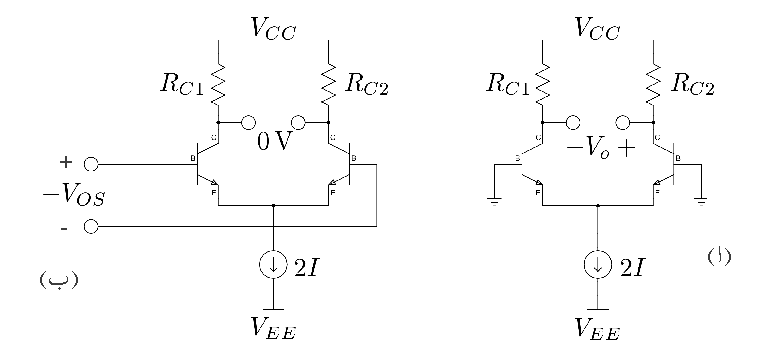
\includegraphics[scale=0.90]{differencePairInputOffsetVoltage}
\caption{داخلی انحرافی برقی دباو}
\label{شکل_تفرقی_جوڑے_کی_داخلی_انحرافی_برقی_دباو}
\end{figure}
\اصطلاح {انحرافی برقی دباو} تفرقی جوڑے کے مزاحمت \عددی{R_{C1}} اور \عددی{R_{C2}} برابر نہ ہونے سے پیدا ہوتا ہے۔اسی طرح \عددی{Q_1} اور \عددی{Q_2} یکساں نہ ہونے سے بھی \اصطلاح {انحرافی برقی دباو} جنم لیتا ہے۔آئیں ان پر غور کریں۔

تفرقی جوڑے کے دو ٹرانزسٹر مکمل طور یکساں ہونے کی صورت میں اگر اس کے دونوں داخلی سرے برقی زمین پر رکھے جائیں (یعنی \عددی{V_{B1}=V_{B2}=0} ) تو برقی رو \عددی{2 \times I} ان میں برابر تقسیم ہو گی۔ اگر \عددی{R_{C1}} اور \عددی{R_{C2}} کی قیمتیں بھی بالکل برابر ہوں تو \عددی{V_{C1}} اور \عددی{V_{C2}} برابر ہوں گے اور یوں \عددی{V_o=0} ہو گا۔البتہ اگر \عددی{R_{C1}} اور \عددی{R_{C2}} کی قیمتیں مختلف ہوں مثلاً
\begin{gather}
\begin{aligned}
R_{C1}&=R_C + \Delta R_C\\
R_{C2}&=R_C-\Delta R_C
\end{aligned}
\end{gather}
تب
\begin{gather}
\begin{aligned}
V_{C1}&=V_{CC}-\alpha I R_{C1}=V_{CC}-\alpha I \left (R_C + \Delta R_c \right )\\
V_{C2}&=V_{CC}-\alpha I R_{C2}=V_{CC}-\alpha I \left (R_C - \Delta R_c \right )
\end{aligned}
\end{gather}
ہوں گے اور یوں
\begin{align}
V_o=V_{C2}-V_{C1}=2 \alpha I \Delta R_C
\end{align}
ہو گا۔یہ \اصطلاح {خارجی انحرافی برقی دباو} ہے جس سے \اصطلاح {داخلی انحرافی برقی دباو} یوں حاصل ہوتا ہے۔
\begin{align}
V_{OS}=\frac{V_O}{ A_d}=\frac{2 \alpha I \Delta R_C}{g_m R_C} = \frac{2 \alpha I \Delta R_C}{\left( \frac{\alpha I}{V_T} \right ) R_C} =2 V_T \frac{\Delta R_C}{R_C}
\end{align}
اس مساوات کے حصول میں \عددی{A_d = g_m R_C} اور \عددی{g_m = \frac{\alpha I}{V_T}} کا استعمال کیا گیا ہے۔داخلی انحرافی برقی دباو کو بطور مثبت عدد لکھا جاتا ہے یعنی
\begin{align}
\abs{V_{OS}}=\abs{2 V_T \frac{\Delta R_C}{R_C}}
\end{align}
آئیں اب ٹرانزسٹر یکساں نہ ہونے سے پیدا انحرافی برقی دباو پر غور کریں۔ فرض کریں کہ ٹرانزسٹر کے \عددی{I_S} مختلف ہیں یعنی
\begin{gather}
\begin{aligned}
I_{S1}&=I_S+\Delta I_S \\
I_{S2}&=I_S - \Delta I_S
\end{aligned}
\end{gather}
ہیں۔شکل \حوالہ{شکل_تفرقی_جوڑے_کی_داخلی_انحرافی_برقی_دباو} الف میں ٹرانزسٹر کے ایمٹر سرے آپس میں جڑے ہیں جبکہ ان کے بیس  سرے برقی زمین پر ہیں۔یوں \عددی{V_{BE1}=V_{BE2}=V_{BE}} ہے۔اس صورت ٹرانزسٹر کی برقی رو مندرجہ ذیل ہوں گی۔
\begin{gather}
\begin{aligned}
I_{C1}&=\left(I_S + \Delta I_S \right ) \left (e^{\frac{V_{BE}}{V_T}} -1\right )\\
I_{C2}&=\left(I_S - \Delta I_S \right ) \left (e^{\frac{V_{BE}}{V_T}-1} \right )
\end{aligned}
\end{gather}
ان سے \عددی{\frac{I_{C2}}{I_{C1}}} حاصل کرتے ہیں۔
\begin{align}
\frac{I_{C2}}{I_{C1}}=\frac{I_S-\Delta I_S}{I_S + \Delta I_S}
\end{align}
دونوں جانب ایک \عددی{(1)}  جمع کرتے ہیں۔
\begin{gather}
\begin{aligned}
\frac{I_{C2}}{I_{C1}}+1 &=1+\frac{I_S - \Delta I_S}{I_S + \Delta I_S}\\
\frac{I_{C2}+I_{C1}}{I_{C1}}&=\frac{2 I_S}{I_S + \Delta I_S}
\end{aligned}
\end{gather}
چونکہ \عددی{I_{C1}+I_{C2}=2 \times I \times \alpha}  ہے لہٰذا اس مساوات سے حاصل ہوتا ہے۔
\begin{align}
I_{C1}= I \times \alpha \left(\frac{I_S + \Delta I_S}{I_S} \right )=\alpha I \left (1+\frac{\Delta I_S}{I_S} \right )
\end{align}
اسی طرح \عددی{I_{C2}}  کے لئے حاصل ہو گا۔
\begin{align}
I_{C2}=I \times \alpha \left(\frac{I_S - \Delta I_S}{I_S} \right )=\alpha I \left (1-\frac{\Delta I_S}{I_S} \right )
\end{align}
اور
\begin{gather}
\begin{aligned}
V_{C1}&=V_{CC}-\alpha I \left(1+\frac{\Delta I_S}{I_S} \right ) R_C\\
V_{C2}&=V_{CC}-\alpha I \left(1- \frac{\Delta I_S}{I_S} \right ) R_C\\
V_O&=V_{C2}-V_{C1}=2 \alpha I R_C \frac{\Delta I_S}{I_S}\\
\abs{V_{OS}}&=\abs{\frac{V_{O}}{A_d}}=\abs{\frac{V_O}{g_m R_C}}=\abs{\frac{2 \alpha I R_C \frac{\Delta I_S}{I_S}}{\frac{\alpha I}{V_T} R_C}}=\abs{2 V_T \frac{\Delta I_S}{I_S}}
\end{aligned}
\end{gather}
ان دو وجوہات کے علاوہ دیگر وجوہات (مثلاً \عددی{\beta}  اور \عددی{r_o} میں فرق) کے بنا پر بھی انحرافی برقی دباو پیدا ہوتا ہے۔

\جزوحصہ{داخلی میلان برقی رو اور انحرافی داخلی میلان برقی رو}
تفرقی جوڑے کے دونوں بازو مکمل یکساں ہونے کی صورت میں دونوں جانب برابر یک سمت \اصطلاح {میلان برقی رو}\فرہنگ{میلان برقی رو}\فرہنگ{input bias current}\حاشیہب{input bias current} کا گزر ہوتا ہے یعنی
\begin{align}
I_{B1}=I_{B2}=\frac{I}{\beta+1}
\end{align}
البتہ دونوں بازووں میں فرق کی بنا پر دونوں جانب کی \اصطلاح {داخلی میلان برقی رو} مختلف ہو سکتی ہیں۔ایسی صورت میں دونوں جانب کی \اصطلاح {داخلی میلان برقی رو} میں فرق، جسے  \اصطلاح {انحرافی داخلی برقی رو}\فرہنگ{انحرافی برقی رو}\فرہنگ{input offset current}\حاشیہب{input offset curent}  \عددی{I_{OS}}  کہتے ہیں، کو یوں حاصل کرتے ہیں۔
\begin{align}
I_{OS}=\abs{I_{B1}-I_{B2}}
\end{align}
ٹرانزسٹر کے \عددی{\beta}  میں اس کے عمومی قیمت سے انحراف کو دیکھتے ہیں۔تصور کریں کہ
\begin{gather}
\begin{aligned}
\beta_1 &=\beta+\Delta \beta \\
\beta_2 &=\beta - \Delta \beta
\end{aligned}
\end{gather}
 ہیں جہاں \عددی{\beta} اس کی عمومی قیمت ہے اور \عددی{\Delta \beta} اس عمومی قیمت سے انحراف ہے۔اس طرح
\begin{gather}
\begin{aligned}\label{مساوات_تفرقی_افزائش_لمبی_تقسیم_الف}
I_{B1}&=\frac{I}{\beta+\Delta \beta +1}=\frac{I}{\left(\beta+1 \right ) \left(1+\frac{\Delta \beta}{\beta+1} \right )} \approx \frac{I}{\beta+1} \left (1-\frac{\Delta \beta}{\beta+1} \right )\\
I_{B2}&=\frac{I}{\beta - \Delta \beta +1}=\frac{I}{\left(\beta+1 \right ) \left(1 - \frac{\Delta \beta}{\beta+1} \right )} \approx \frac{I}{\beta+1} \left (1+ \frac{\Delta \beta}{\beta+1} \right )\\
\end{aligned}
\end{gather}
ہوں گے۔مساوات \حوالہ{مساوات_تفرقی_افزائش_لمبی_تقسیم_الف} کے دوسرے مساوات میں \عددی{\frac{\Delta \beta}{\beta+1}} کو \عددی{x} تصور کرتے ہوئے شکل \حوالہ{شکل_لمبی_تقسیم} میں دکھائے لمبی تقسیم کے طرز  پر حل کرتے ہوئے  صرف پہلے دو جزو لیتے ہوئے \عددی{\tfrac{1}{1-\tfrac{\Delta \beta}{\beta+1}}\approx 1+\tfrac{\Delta \beta}{\beta+1}} لکھا گیا ہے۔مساوات \حوالہ{مساوات_تفرقی_افزائش_لمبی_تقسیم_الف} کے پہلے مساوات میں بھی یہی ترقیب استعمال کی گئی ہے۔
\begin{figure}
\centering
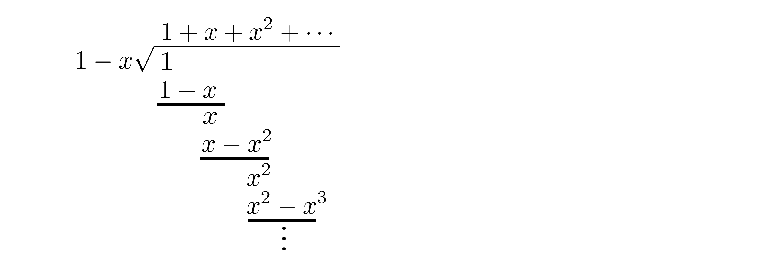
\includegraphics[scale=0.90]{longDivision}
\caption{لمبی تقسیم}
\label{شکل_لمبی_تقسیم}
\end{figure}
اس طرح
\begin{align}
I_B=\frac{I_{B1}+I_{B2}}{2}=\frac{I}{\beta+1}
\end{align}
اور
\begin{align}
I_{OS}=\abs{\frac{2 I}{\beta+1} \left(\frac{\Delta \beta}{\beta+1} \right )}=2 I_B \left(\frac{\Delta \beta}{\beta+1} \right )
\end{align}
حاصل ہوتے ہیں۔

\حصہ{مخلوط ادوار میں دو جوڑ ٹرانزسٹر کے مائل کرنے کے طریقے}
ہم نے دو جوڑ ٹرانزسٹر کو چار عدد مزاحمت کے مدد سے مائل کر کے ان کے نقطہ کارکردگی تعین کرنا دیکھا۔مخلوط دور میں ٹرانزسٹر کے نسبت، مزاحمت بنانا زیادہ مہنگا ثابت ہوتا ہے۔اسی لئے مخلوط ادوار میں مزاحمت کے استعمال سے گریز کیا جاتا ہے اور ان میں ٹرانزسٹر کو \اصطلاح {یک سمت  منبع رو}\فرہنگ{یک سمت  منبع رو}\فرہنگ{constant current source}\حاشیہب{constant current source}  کی مدد سے مائل کیا جاتا ہے۔اس سے پہلے کہ ہم دیکھیں یہ کیسا کیا جاتا ہے یہ ضروری ہے کہ \اصطلاح {یک سمت  منبع رو} پر غور کیا جائے۔

\حصہ{یک سمت  منبع برقی رو}
شکل  \حوالہ{شکل_پیداکار_مستقل_برقی_رو} الف میں \عددی{npn}  ٹرانزسٹر استعمال کرتے ہوئے \اصطلاح {یک سمت  منبع رو} کا حصول دکھایا گیا ہے۔ اس دور میں، \عددی{\alpha} کو تقریباً ایک \عددی{(\approx 1)}  تصور کرتے ہوئے، جب تک ٹرانزسٹر افزائندہ  رہے، \عددی{I_{\textup{بوجھ} }}  کا دارومدار زینر ڈایوڈ کے \عددی{V_Z} اور مزاحمت \عددی{R_E} پر ہے یعنی
\begin{align*}
I_E=\frac{V_Z-V_{BE}}{R_E}
\end{align*}
یوں \عددی{I_{\textup{بوجھ} }}  تبدیل کرنے سے اس میں برقی رو تبدیل نہیں ہوتی۔اس سے ہم دیکھ سکتے ہیں کہ \عددی{I_{\textup{بوجھ} }}   سے منسلک بقایا دور بطور \اصطلاح {یک سمت  منبع رو} کام کرتا ہے۔شکل میں نقطہ دار دائرے میں بند حصے کو \اصطلاح {یک سمت  منبع رو} کہتے ہیں۔
شکل \حوالہ{شکل_پیداکار_مستقل_برقی_رو} ب میں \اصطلاح {یک سمت  منبع رو} کی علامت (تیر والا دائرہ) استعمال کرتے ہوئے اسی دور کو دوبارہ پیش کیا گیا ہے۔علامت میں تیر کا نشان مستقل برقی رو کی سمت دکھلاتا ہے۔آپ دیکھ سکتے ہیں کہ اس طرز کے یک سمت  منبع رو کو استعمال کرتے ہوئے بوجھ کو مثبت برقی دباو \عددی{V_{CC}} اور یک سمت  منبع رو کے مابین نسب کیا جاتا ہے اور یک سمت  منبع رو  کی سمت بوجھ سے یک سمت  منبع رو کی جانب ہوتی ہے۔یہاں آپ دیکھ سکتے ہیں کہ بوجھ سے برقی رو خارج ہو کر یک سمت  منبع رو میں داخل ہوتی ہے۔ایسی یک سمت  منبع رو بوجھ سے برقی رو زبردستی خارج  کراتی ہے۔اسی لئے اس دور کا زیادہ مقبول نام \اصطلاح {خارج کار منبع رو}\فرہنگ{خارج کار منبع رو}\حاشیہب{current sink}\فرہنگ{current sink} ہے۔ 
\begin{figure}
\centering
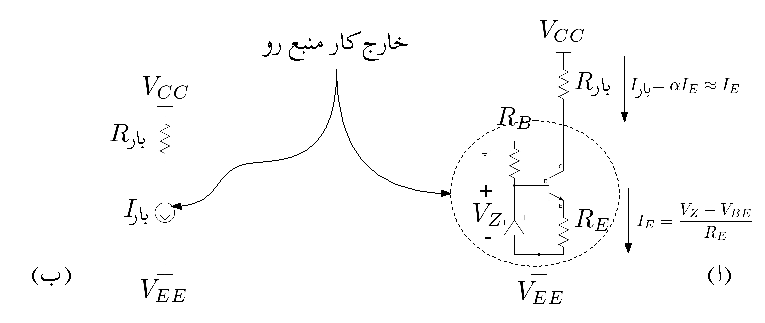
\includegraphics[scale=0.90]{constantCurrentSourceA}
\caption{خارج کار منبع رو}
\label{شکل_پیداکار_مستقل_برقی_رو}
\end{figure}
شکل-\حوالہ{شکل_پیداکار_مستقل_برقی_رو_ب} الف میں \عددی{pnp} ٹرانزسٹر پر مبنی یک سمت  منبع رو دکھایا گیا ہے جبکہ شکل \حوالہ{شکل_پیداکار_مستقل_برقی_رو_ب} ب میں اسی دور کی علامتی شکل دکھائی گئی ہے۔اس طرز کے یک سمت  منبع رو کو استعمال کرتے ہوئے بوجھ کو یک سمت  منبع رو اور منفی برقی دباو \عددی{V_{EE}}  کے مابین نسب کیا جاتا ہے اور یک سمت  منبع رو  کی سمت یک سمت  منبع رو سے بوجھ کی جانب ہوتی ہے۔ایسی یک سمت  منبع رو بوجھ میں برقی رو زبردستی داخل  کرتی ہے۔اسی لئے اس دور کو \اصطلاح {داخل کار منبع رو}\فرہنگ{داخل کار منبع رو}\حاشیہب{current source}\فرہنگ{current source} بھی کہا جاتا ہے۔ 
\begin{figure}
\centering
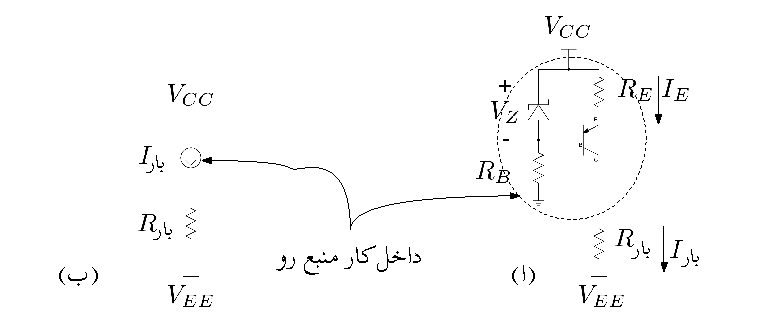
\includegraphics[scale=0.90]{constantCurrentSourceB}
\caption{داخل کار برقی رو}
\label{شکل_پیداکار_مستقل_برقی_رو_ب}
\end{figure}

مخلوط ادوار میں عموماً متعدد یک سمت  منبع رو درکار ہوتے ہیں۔وقت کے ساتھ ایسے ادوار کے کارکردگی میں تبدیلی آتی ہے جسے \اصطلاح {عمر رسیدگی}\فرہنگ{عمر رسیدگی}\فرہنگ{ageing}\حاشیہب{ageing}  کا عمل کہتے ہیں۔اسی طرح درجہ حرارت اور دیگر وجوہات کی بنا پر بھی ادوار کے کارکردگی میں تبدیلی رونما ہوتی ہے۔مخلوط دور میں استعمال ہونے والے تمام یک سمت  منبع رو میں پائے جانے والے اس طرح کے اثرات کو یکساں بنانے کی کوشش کی جاتی ہے۔یوں ان سے نپٹنا نسبتاً آسان ہوتا ہے۔آئیں دیکھیں کہ اس طرز کے یک سمت  منبع رو کیسے بنائے جاتے ہیں۔

\حصہ{آئینہ برقی رو}
شکل \حوالہ{شکل_آئینہ_برقی_رو_الف} الف میں \اصطلاح {آئینہ برقی رو}\فرہنگ{آئینہ برقی رو}\فرہنگ{current mirror}\حاشیہب{current mirror}  دکھایا گیا ہے۔تصور کریں کہ دونوں ٹرانزسٹر کے \عددی{\beta} کی قیمت لامحدود ہے اور بائیں بازو میں برقی رو  \عددی{I_{\textup{حوالہ}}} گزر رہی ہے۔ \عددی{\beta} کی قیمت لامحدود ہو تو ٹرانزسٹر کے بیس  سرے پر برقی رو  \عددی{I_B}  قابل نظر انداز ہو گی۔یوں ٹرانزسٹر \عددی{Q_1}  میں برقی رو  \عددی{I_{\textup{حوالہ}}}  اور اس کے بیس-ایمٹر جوڑ پر برقی دباو \عددی{V_{BE}} پایا جائے گا جہاں
\begin{align} \label{مساوات_تفرقی_حوالہ_رو}
I_{\textup{حوالہ}}=I_S \left(e^{\frac{V_{BE}}{V_T}}-1 \right )
\end{align}
%
\begin{figure}
\centering
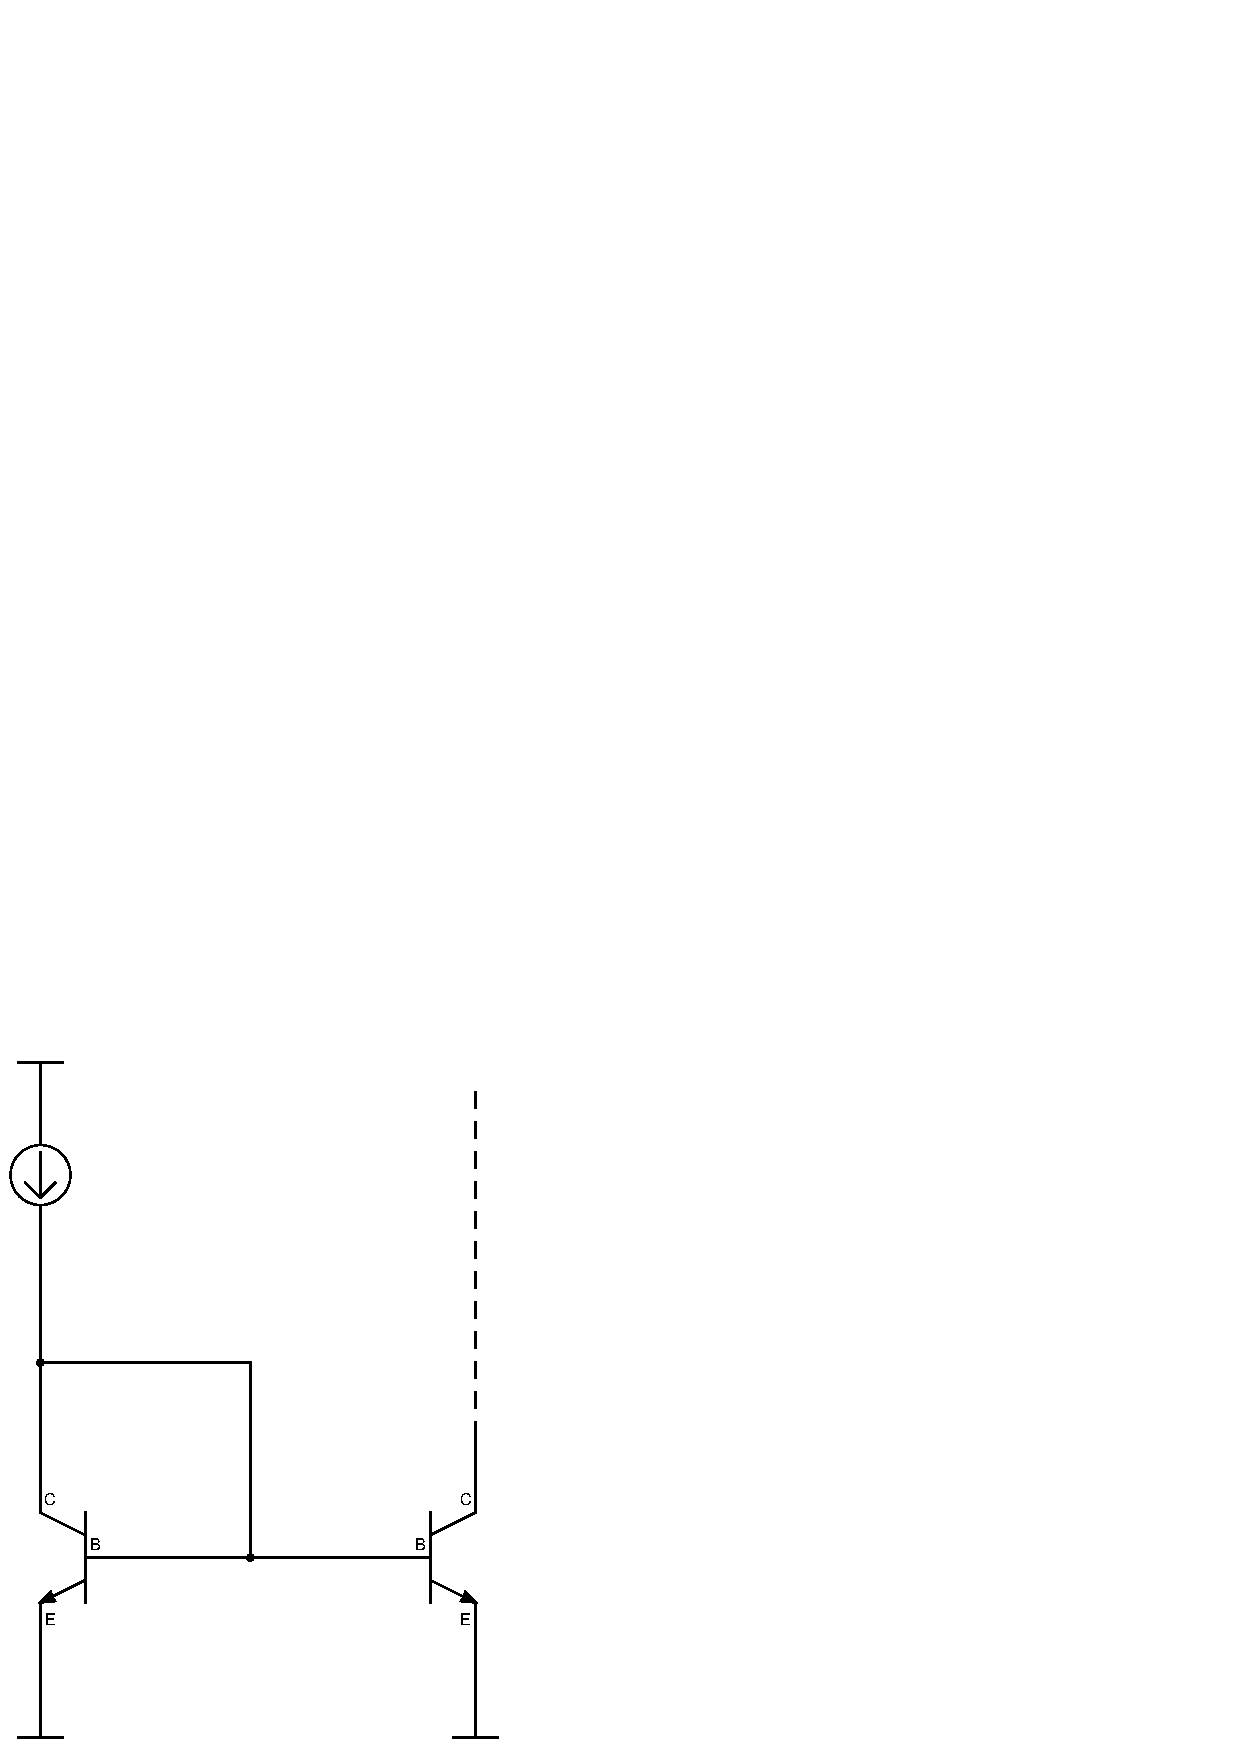
\includegraphics[scale=0.90]{currentMirrorA}
\caption{ آئینہ برقی رو}
\label{شکل_آئینہ_برقی_رو_الف}
\end{figure}
ٹرانزسٹر \عددی{Q_1} اور \عددی{Q_2} کے بیس  سرے آپس میں جڑے ہیں۔اسی طرح ان کے ایمٹر سرے بھی آپس میں جڑے ہیں۔یوں \عددی{Q_2}  کے بیس-ایمٹر جوڑ پر بھی برقی دباو \عددی{V_{BE}} ہی پایا جائے گا۔اس ٹرانزسٹر کے لئے ہم لکھ سکتے ہیں۔
\begin{align} \label{مساوات_تفرقی_عکس_رو}
I_{\textup{عکس}}=I_S \left(e^{\frac{V_{BE}}{V_T}}-1 \right )
\end{align}
مساوات \حوالہ{مساوات_تفرقی_عکس_رو} کو مساوات \حوالہ{مساوات_تفرقی_حوالہ_رو}  سے تقسیم کرتے ملتا ہے۔
\begin{gather}
\begin{aligned}
\frac{I_{\textup{عکس}}}{I_{\textup{حوالہ}}}&=\frac{I_S \left(e^{\frac{V_{BE}}{V_T}}-1 \right )}{I_S \left(e^{\frac{V_{BE}}{V_T}}-1 \right )}=1\\
I_{\textup{عکس}}&=I_{\textup{حوالہ}}
\end{aligned}
\end{gather}
یوں \عددی{I_{\textup{عکس}}}  بالکل \عددی{I_{\textup{حوالہ}}}  کا \اصطلاح {عکس} ہے۔اس کو یوں بھی بیان کر سکتے ہیں کہ بوجھ میں  \عددی{I_{\textup{حوالہ}}} کے \اصطلاح {حوالے} سے برقی رو گزرتی ہے۔جیسا کہ مثال \حوالہ{مثال_تفرقی_عکس_الف}  میں واضح کیا گیا ہے \اصطلاح {آئینہ برقی رو} کی صحیح کارکردگی کے لئے یہ ضروری ہے کہ \عددی{Q_2} کو افزائندہ رکھا جائے۔

محدود \عددی{\beta} کی وجہ سے \عددی{I_{\textup{عکس}}}  اور \عددی{I_{\textup{حوالہ}}} میں معمولی فرق رہتا ہے جس کی شکل  ب میں وضاحت کی گئی ہے۔چونکہ دونوں جانب ٹرانزسٹر کے بیس-ایمٹر جوڑ پر یکساں برقی دباو \عددی{V_{BE}} پایا جاتا ہے لہٰذا ان دونوں کے کلکٹر سروں پر برابر برقی رو \عددی{I_C} پائی جائے گی۔یعنی
\begin{gather}
\begin{aligned}
I_{C1}&=I_S \left(e^{\frac{V_{BE}}{V_T}}-1 \right )\\
I_{C2}&=I_S \left(e^{\frac{V_{BE}}{V_T}}-1 \right )\\
I_{C1}&=I_{C2}=I_C
\end{aligned}
\end{gather}
اسی طرح ان کے بیس  سروں پر بھی برابر برقی رو پائی جائے گی یعنی
\begin{gather}
\begin{aligned}
I_{B1}&=\frac{I_{C1}}{\beta}=\frac{I_C}{\beta}\\
I_{B2}&=\frac{I_{C2}}{\beta}=\frac{I_C}{\beta}
\end{aligned}
\end{gather}
بائیں بازو کرخوف کے قانون برائے برقی رو کے تحت
\begin{align}
I_{\textup{حوالہ}}=I_C+\frac{2 I_C}{\beta}=I_C \left(1+\frac{2}{\beta} \right )
\end{align}
جبکہ دائیں بازو
\begin{align}
I_{\textup{عکس}}=I_{C2}=I_C
\end{align}
یوں
\begin{align} \label{مساوات_تفرقی_عکس_رو_الف}
I_{\textup{عکس}}=\frac{I_{\textup{حوالہ}}}{1+\frac{2}{\beta}}
\end{align}
ہو گا۔جیسے آپ دیکھ سکتے ہیں کہ دونوں بازووں کی برقی رو میں ٹرانزسٹر کے بیس  سرے کی برقی رو کی وجہ سے فرق پایا جاتا ہے۔شکل \حوالہ{شکل_بہتر_پیداکار_مستقل_برقی_رو}   میں اس اثر کو کم کرنے کی ترکیب دکھائی گئی ہے جہاں سے ظاہر ہے کہ
\begin{align}\label{مساوات_تفرقی_بہتر_آئینہ_کی_مساوات}
I_{\textup{عکس}} \approx \frac{I_{\textup{حوالہ}}} {1+\frac{2}{\beta^2}}
\end{align}
اس مساوات کو مساوات \حوالہ{مساوات_تفرقی_عکس_رو_الف}  کے ساتھ دیکھیں۔ فرق کے مقدار کو \عددی{\beta} گنا کم کر دیا گیا ہے۔
\begin{figure}
\centering
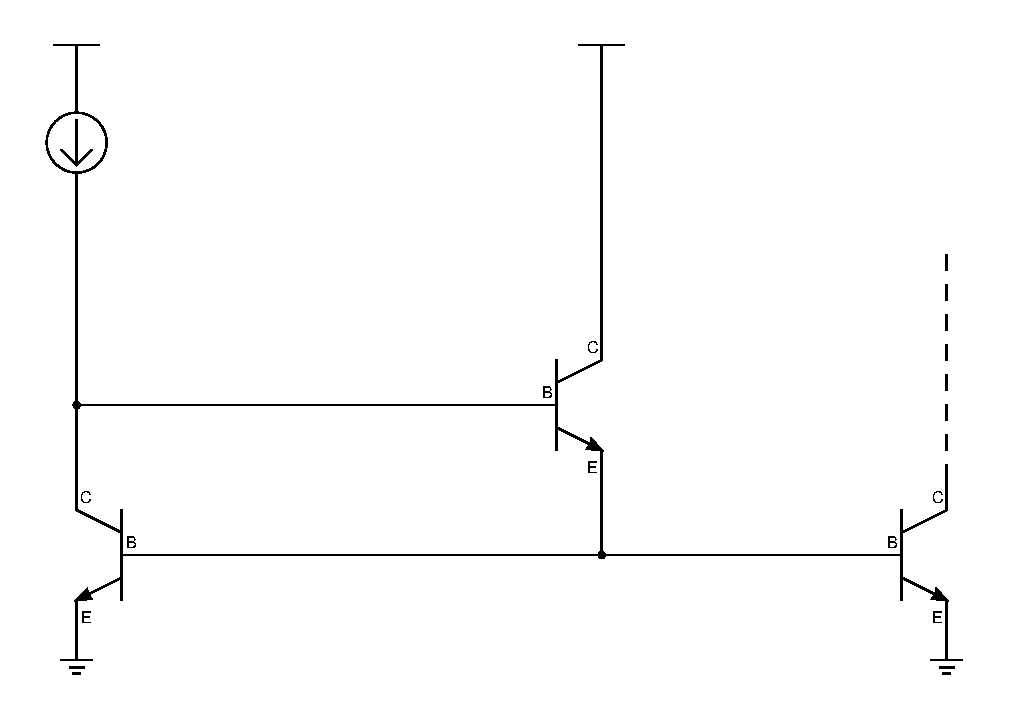
\includegraphics[scale=0.90]{currentMirrorB}
\caption{بہتر یک سمت  منبع رو}
\label{شکل_بہتر_پیداکار_مستقل_برقی_رو}
\end{figure}
اگر شکل \حوالہ{شکل_بہتر_پیداکار_مستقل_برقی_رو} میں \عددی{I_{\textup{حوالہ}}} پیدا کرنے کی خاطر ایک عدد مزاحمت \عددی{R}  کو \عددی{V_{CC}} اور \عددی{Q_3} کے کلکٹر سرے کے درمیان جوڑ دیا جائے تب \عددی{I_{\textup{حوالہ}}}  یوں حاصل ہو گا۔
\begin{align}
I_{\textup{حوالہ}}=\frac{V_{CC}-V_{BE1}-V_{BE3}}{R}
\end{align}
%=====

\ابتدا{مثال} \شناخت{مثال_تفرقی_عکس_الف}
شکل \حوالہ{شکل_پیداکار_مستقل_برقی_رو_اور_اس_کی_علامت} الف میں، نقطہ دار لکیر میں بند، ایک سادہ خارج کار مستقل برقی رو دکھایا گیا ہے جسے استعمال کرتے ہوئے برقی بوجھ \عددی{R_{\textup{بوجھ} }} میں برقی رو \عددی{I_{\textup{عکس}}}  گزاری جا رہی ہے۔شکل  ب میں خارج کار مستقل برقی رو کی علامت استعمال کرتے ہوئے اسی دور کو دوبارہ پیش کیا گیا ہے۔اگر 
\begin{align*}
R&=\SI{11.3}{\kilo \ohm}\\
R_{\textup{بوجھ} }&=\SI{5}{\kilo \ohm}
\end{align*}
ہوں تو 
\begin{enumerate}
\item
برقی بوجھ \عددی{R_{\textup{بوجھ} }} میں برقی رو \عددی{I_{\textup{عکس}}}  حاصل کریں۔
\item
برقی دباو \عددی{V_o} حاصل کریں۔
\item
اگر \عددی{R_{\textup{بوجھ} }} کی مزاحمت دگنی کر دی جائے تب \عددی{V_o} کی قیمت کیا ہو گی۔
\item
\عددی{R_{\textup{بوجھ} }} کی مزاحمت \عددی{\SI{20}{\kilo \ohm}} ہونے کی صورت میں \عددی{V_o} کی قیمت حاصل کریں۔
\item
برقی بوجھ \عددی{R_{\textup{بوجھ}}} کی وہ مزاحمت دریافت کریں جس پر ٹرانزسٹر \عددی{Q_2} غیر افزائندہ حال ہو جاتا ہے۔
\item
برقی بوجھ کی مزاحمت \عددی{\SI{40}{\kilo \ohm}} کرنے سے کیا نتائج مرتب ہوں گے۔

\end{enumerate}

\begin{figure}
\centering
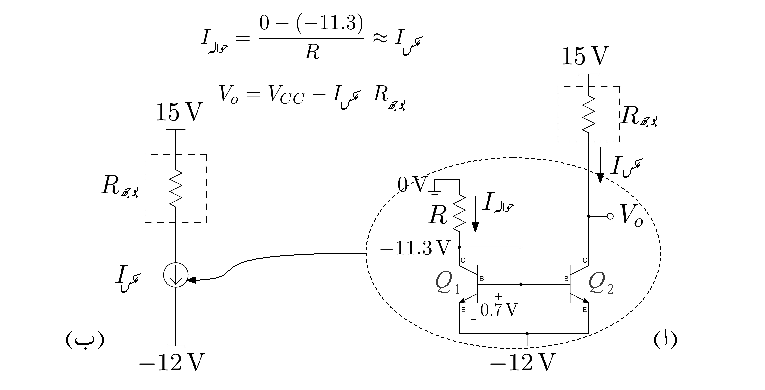
\includegraphics[scale=0.90]{currentMirrorC}
\caption{خارج کار مستقل برقی رو اور اس کی علامت}
\label{شکل_پیداکار_مستقل_برقی_رو_اور_اس_کی_علامت}
\end{figure}

حل:
\begin{enumerate}
\item
ٹرانزسٹر \عددی{Q_1}  کا ایمٹر سرا \عددی{\SI{-12}{\volt}}   پر ہے جبکہ اس کے بیس-ایمٹر جوڑ پر \عددی{\SI{0.7}{\volt}} پائے جاتے ہیں۔یوں اس کا بیس  سرا  \عددی{\SI{-11.3}{\volt}} پر ہو گا۔چونکہ بیس اور کلکٹر جڑے ہیں لہٰذا کلکٹر بھی  \عددی{\SI{-11.3}{\volt}} پر ہو گا۔یوں مزاحمت \عددی{R}  کے ایک سرے پر  \عددی{\SI{-11.3}{\volt}} ہیں۔مزاحمت کا دوسرا سرا برقی زمین پر ہے اور یوں اس پر  \عددی{\SI{0}{\volt}} ہے۔ مزاحمت \عددی{R} میں برقی رو
\begin{align*}
I_{\textup{حوالہ}}=\frac{0-(-11.3)}{11300}=\SI{1}{\milli \ampere}
\end{align*}
پائی جائے گی۔ برقی بوجھ \عددی{R_{\textup{بوجھ} }} سے بھی ایک ملی ایمپیئر کی برقی رو گزرے گی۔
\item
ٹرانزسٹر \عددی{Q_2}  کے کلکٹر سرے پر برقی دباو
\begin{align*}
V_o&=V_{CC}-I_{\textup{عکس}} R_{\textup{بوجھ} }\\
&=15-10^{-3} \times 5 \times 10^{3}=\SI{10}{\volt}
\end{align*}
پایا جاتا ہے۔
\item
برقی بوجھ کی مزاحمت دگنی یعنی \عددی{\SI{10}{\kilo \ohm}} کرنے سے
\begin{align*}
V_o&=V_{CC}-I_{\textup{عکس}} R_{\textup{بوجھ} }\\
&=15-10^{-3} \times 2 \times 5 \times 10^{3}=\SI{5}{\volt}
\end{align*}
\item
برقی بوجھ کی مزاحمت \عددی{\SI{20}{\kilo \ohm}} کرنے سے
\begin{align*}
V_o&=V_{CC}-I_{\textup{عکس}} R_{\textup{بوجھ} }\\
&=15-10^{-3} \times 20 \times 10^{3}=\SI{-5}{\volt}
\end{align*}
ہو گا۔
\item
اس مثال کے جزو ب، پ اور ت میں ہم دیکھتے ہیں کہ جب برقی بوجھ \عددی{R_{\textup{بوجھ} }}  کی مزاحمت بڑھائی جائے تو خارج کار مستقل برقی رو برقی دباو  \عددی{V_o} گھٹا کر برقی بوجھ میں برقی رو کی قیمت برقرار رکھتا ہے۔آپ دیکھ سکتے ہیں کہ اگر برقی بوجھ کی مزاحمت اسی طرح بتدریج بڑھائی جائے تو آخر کار \عددی{Q_2} غیر افزائندہ خطے میں داخل ہو جائے گا  اور اس کے لئے \عددی{V_o} کا مزید گھٹانا ممکن نہ ہو گا۔ٹرانزسٹر \عددی{Q_2} غیر افزائندہ ہونے کے بعد اگر برقی بوجھ کی مزاحمت مزید بڑھائی جائے تو اس میں برقی رو گھٹنا شروع ہو جائے گی۔

ٹرانزسٹر \عددی{Q_2} اس صورت غیر افزائندہ ہو گا جب اس کے کلکٹر-ایمٹر   سروں کے مابین \عددی{\SI{0.2}{\volt}} پائے جائیں۔اس صورت میں اگر گزشتہ جزو  کے مساوات کو \عددی{R_{\textup{بوجھ} }} کے لئے حل کریں تو حاصل ہوتا ہے
\begin{align*}
15&=I_{\textup{عکس}} R_{\textup{بوجھ} } +V_{\textup{CEغیرافزائندہ}} -12\\
15&=10^{-3} \times R_{\textup{بوجھ} } + 0.2-12\\
R_{\textup{بوجھ} }&=\frac{15+12-0.2}{10^{-3}}=\SI{26.8}{\kilo \ohm}
\end{align*}
\item
ہم نے دیکھا کہ خارج کار مستقل برقی رو \عددی{\SI{26.8}{\kilo \ohm}} کے برقی بوجھ تک کے مزاحمت میں مستقل برقی رو برقرار رکھ سکتا ہے۔برقی بوجھ کے مزاحمت کو مزید بڑھانے سے برقی بوجھ میں رواں برقی رو گھٹنا شروع ہو جاتی ہے۔ \عددی{\SI{40}{\kilo \ohm}} کے برقی بوجھ کے لئے 
\begin{align*}
15&=I R_{\textup{بوجھ} } +V_{\textup{CEغیرافزائندہ}} -12\\
15&=I \times 40 \times 10^{3}+0.2-12\\
I&=\frac{15+12-0.2}{40 \times 10^{3}}=\SI{0.67}{\milli \ampere}
\end{align*}
ہم دیکھتے ہیں کہ برقی رو کی قیمت \عددی{I_{\textup{اصل}}} سے گھٹ جاتی ہے اور خارج کار مستقل برقی رو صحیح کارکردگی نہیں کر پاتا۔
\end{enumerate}

\انتہا{مثال}
%==========
شکل \حوالہ{شکل_پیداکار_مستقل_برقی_رو_کے_مختلف_ادوار} الف میں \عددی{npn} ٹرانزسٹروں پر مبنی خارج کار مستقل برقی رو دکھایا گیا ہے۔یہ دور نقطہ دار لکیر کی جگہ نسب مطلوبہ دور میں مستقل برقی رو \عددی{I_{\textup{عکس}}} گزارتا ہے۔اس شکل کے لئے ہم لکھ سکتے ہیں۔
\begin{align*}
V_{CC}&=I_{\textup{حوالہ}} R+ V_{BE} +V_{EE}\\
I_{\textup{حوالہ}}&=\frac{V_{CC}-0.7-V_{EE}}{R}=I_{\textup{عکس}}
\end{align*}
%
\begin{figure}
\centering
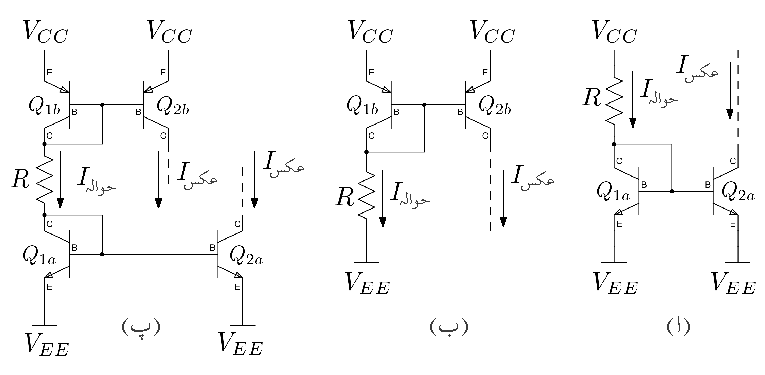
\includegraphics[scale=0.90]{currentMirrorDifferentTypes}
\caption{یک سمت  منبع رو کے مختلف ادوار}
\label{شکل_پیداکار_مستقل_برقی_رو_کے_مختلف_ادوار}
\end{figure}
شکل  ب میں اسی کا مساوی \عددی{pnp}  ٹرانزسٹروں پر مبنی  داخل کار مستقل برقی رو دکھایا گیا ہے۔یہ دور نقطہ دار لکیر کی جگہ نسب مطلوبہ دور میں مستقل برقی رو\عددی{I_{\textup{عکس}}} گزارتا ہے۔

شکل  پ میں ان دونوں ادوار کو یوں جوڑا گیا ہے کہ ایک ہی مزاحمت دونوں یک سمت  منبع رو کے  \عددی{I_{\textup{عکس}}}  کا تعین کرتا ہے۔اس دور کے لئے ہم لکھ سکتے ہیں۔
\begin{align*}
V_{CC}&=V_{EB}+I_{\textup{حوالہ}} R +V_{BE} +V_{EE}\\
I_{\textup{حوالہ}}&=\frac{V_{CC}-0.7-0.7-V_{EE}}{R}=I_{\textup{عکس}}
\end{align*}
\جزوحصہ{متعدد یک سمت  منبع رو}

شکل \حوالہ{شکل_آئینہ_برقی_رو_الف} میں تیسرے ٹرانزسٹر یعنی \عددی{Q_3} کے شمولیت سے شکل \حوالہ{شکل_دو_عکس_کا_حصول} الف حاصل ہوتا ہے۔چونکہ \عددی{Q_3} کے بیس-ایمٹر جوڑ پر بھی \عددی{Q_1} اور \عددی{Q_2} کے برابر \عددی{V_{BE}} پایا جاتا ہے لہٰذا اس میں بھی بالکل انہیں کے برابر \عددی{I_C} برقی رو پائی جائے گی۔
\begin{figure}
\centering
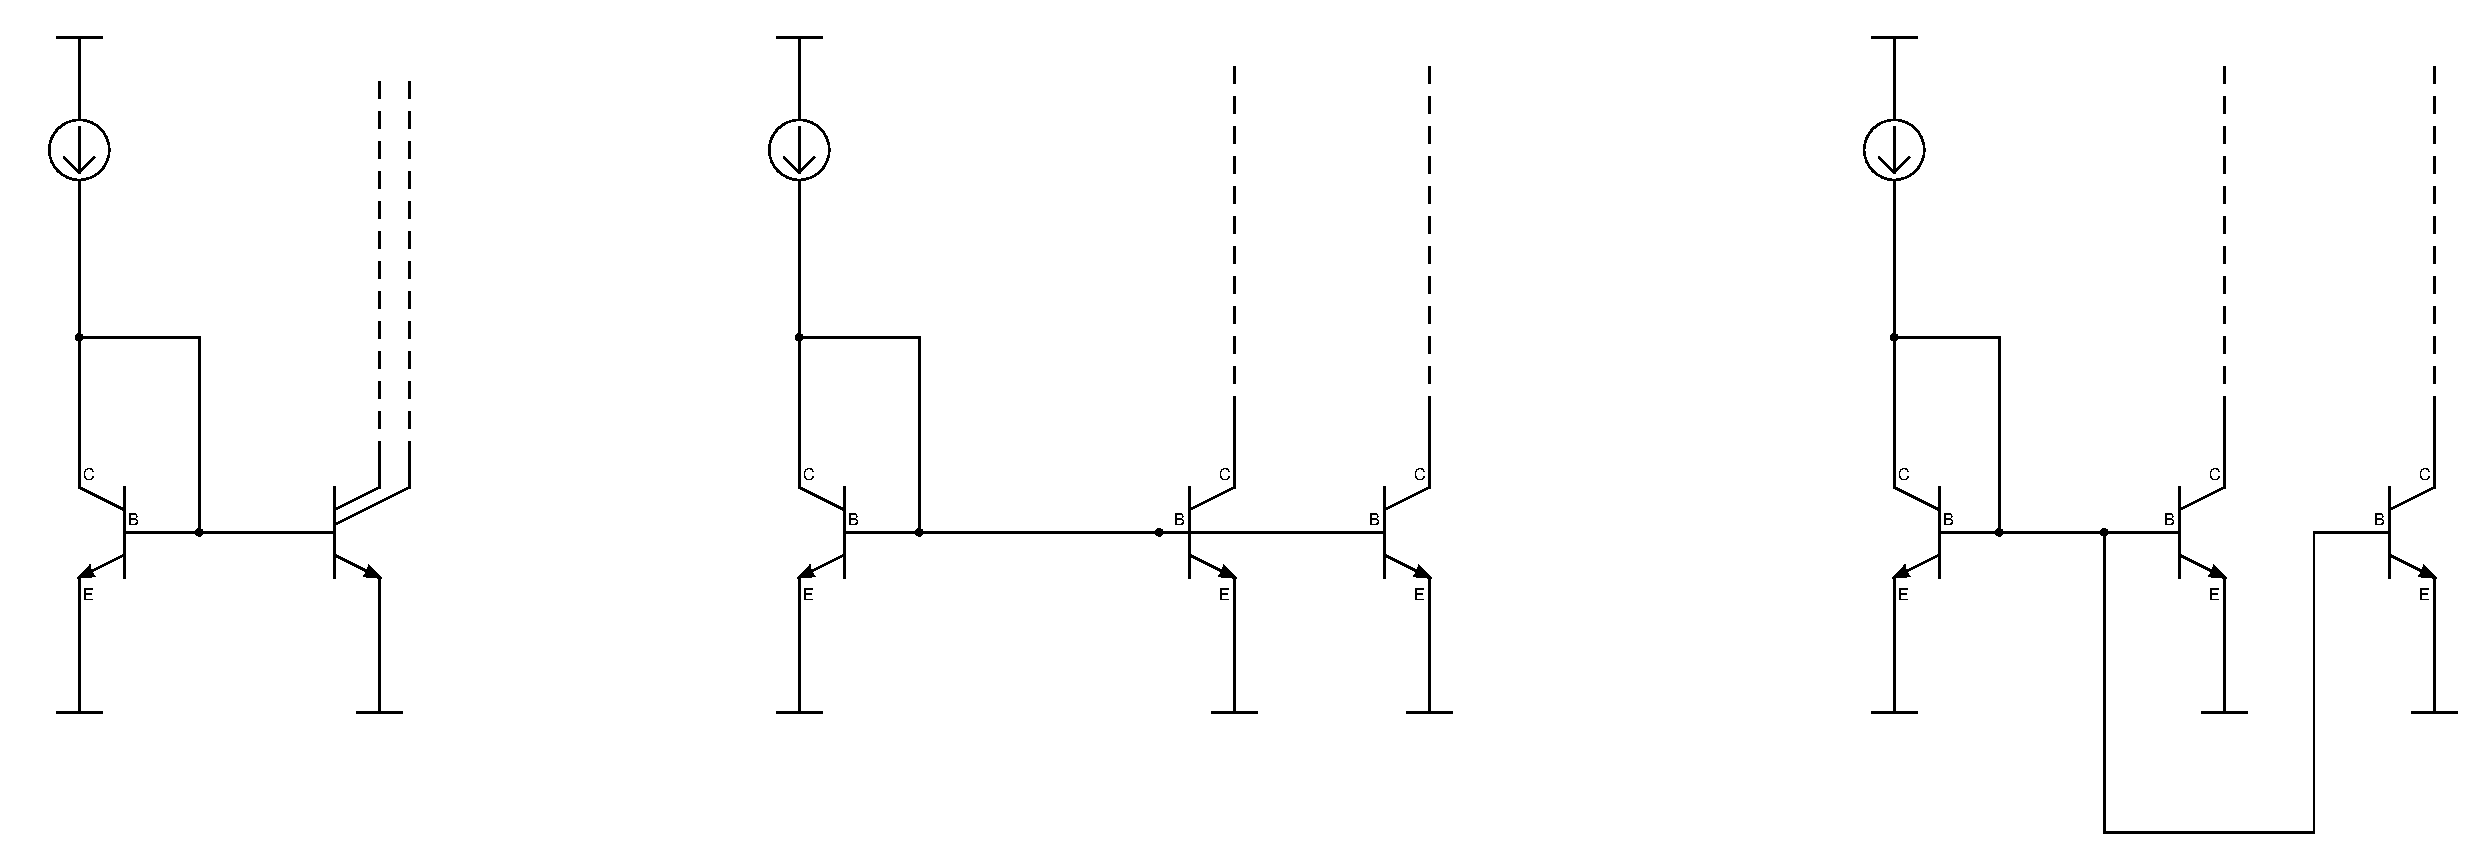
\includegraphics[scale=0.90]{currentMirrorDual}
\caption{دو عکس کا حصول}
\label{شکل_دو_عکس_کا_حصول}
\end{figure}
آئیں دیکھتے ہیں کہ اس دور میں محدود \عددی{\beta} کتنا کردار ادا کرتا ہے۔محدود \عددی{\beta} کی صورت میں ہم لکھ سکتے ہیں کہ
\begin{align}
I_{\textup{1 عکس}}&=I_{\textup{2 عکس}}=I_{\textup{عکس}}=I_C\\
I_{\textup{حوالہ}}&=I_C+\frac{3 I_C}{\beta}
\end{align}
اور یوں
\begin{align} \label{مساوات_تفرقی_تین_عکس}
I_{\textup{عکس}}=\frac{I_{\textup{حوالہ}}}{1+\frac{3}{\beta}}
\end{align}
اس دور کو عموماً شکل \حوالہ{شکل_دو_عکس_کا_حصول} ب یا شکل \حوالہ{شکل_دو_عکس_کا_حصول} پ کے طرز پر صاف اور شفاف طریقے سے بنایا جاتا ہے۔شکل  پ میں ایک ہی ٹرانزسٹر کے دو کلکٹر دکھائے گئے ہیں۔اس سے مراد دو ٹرانزسٹر لینا چاہئے جس کے بیس  آپس میں جڑے ہیں اور اسی طرح اس کے ایمٹر بھی آپس میں جڑے ہیں جبکہ دونوں کے کلکٹر آپس میں نہیں جوڑے گئے ہیں۔

اسی بحث  کو آگے بڑھاتے ہوئے ایک ایسے یک سمت  منبع رو جو \عددی{n} عکس بناتا ہو کے لئے مساوات \حوالہ{مساوات_تفرقی_تین_عکس}  کی صورت یوں ہو گی۔
\begin{align}
I_{\textup{عکس}}=\frac{I_{\textup{حوالہ}}}{1+\frac{n+1}{\beta}}
\end{align}
شکل \حوالہ{شکل_متعدد_پیداکار_برقی_رو}  میں دو یا دو سے زیادہ ٹرانزسٹر جوڑ کر حاصل عکس کو دگنا یا اس سے بھی بڑھانا دکھایا گیا ہے۔
\begin{figure}
\centering
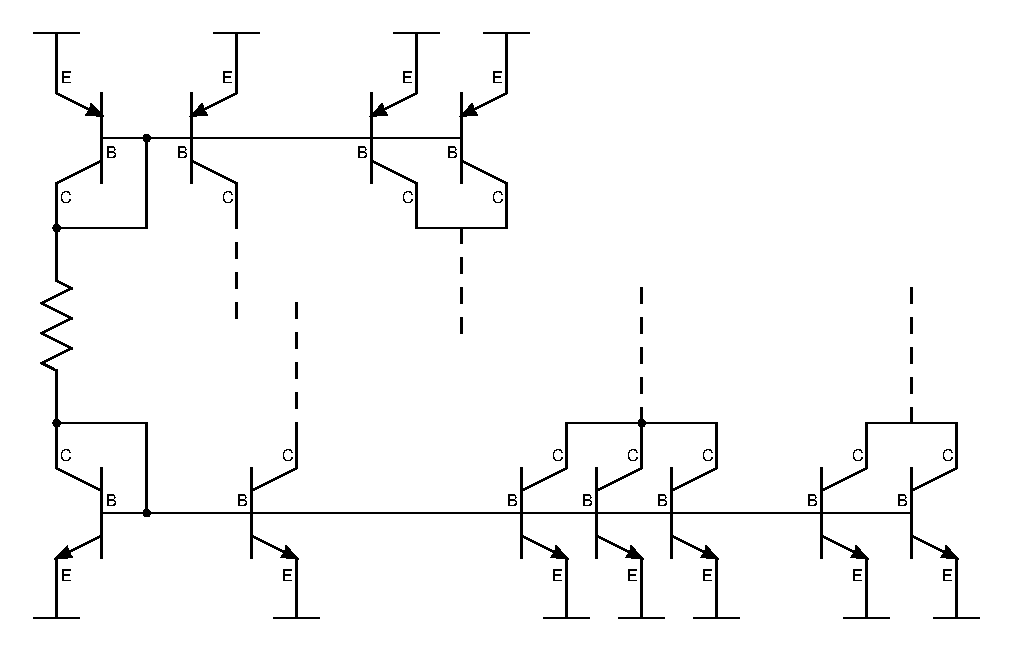
\includegraphics[scale=0.90]{currentMirrorMultiple}
\caption{متعدد یک سمت  منبع رو}
\label{شکل_متعدد_پیداکار_برقی_رو}
\end{figure}
\حصہ{ٹرانزسٹر بوجھ سے لدا دو جوڑ ٹرانزسٹر کا تفرقی ایمپلیفائر}
جیسا کہ پہلے بھی ذکر کیا گیا، مخلوط ادوار بناتے وقت کوشش کی جاتی ہے کہ مزاحمتوں کا استعمال کم سے کم کیا جائے۔جیسا کہ شکل \حوالہ{شکل_ٹرانزسٹر_بار_سے_لدھا_تفرقی_جوڑا} الف میں دکھایا گیا ہے، مخلوط ادوار میں استعمال ہونے والے تفرقی ایمپلیفائر کے خارجی جانب مزاحمت \عددی{R_C} کی جگہ \اصطلاح {آئینہ برقی} رو استعمال کیا جاتا ہے۔

یک سمت  منبع رو کل \عددی{2 \times I} برقی رو جڑوا ٹرانزسٹروں سے گزارتا ہے۔یوں داخلی تفرقی برقی اشارہ کے عدم موجودگی میں ایمپلیفائر کے ٹرانزسٹر \عددی{Q_{a1}}  اور \عددی{Q_{a2}} میں یک سمت برقی رو \عددی{I} گزر کر انہیں مائل کرتی ہے۔ \عددی{Q_{b1}} اور \عددی{Q_{b2}} جو کہ آئینہ برقی رو ہیں، بطورِ برقی بوجھ استعمال کئے گئے ہیں۔ \عددی{Q_{b1}} کی برقی رو کو دیکھ کر \عددی{Q_{b2}} اس کا عکس برقی رو پیدا کرتا ہے۔چونکہ \عددی{Q_{b1}} سے وہی برقی رو گزرتی ہے جو \عددی{Q_{a1}} سے گزرتی ہے لہٰذا \عددی{I} بطور حوالہ استعمال ہو گا اور  \عددی{Q_{b2}} اس کے برابر (یعنی  \عددی{I} ) عکس پیدا کرے گا۔چونکہ  \عددی{Q_{a2}} میں بھی \عددی{I} برقی رو گزر رہی ہے لہٰذا \عددی{Q_{b2}} کی پیدا کردہ تمام کی تمام برقی رو \عددی{Q_{a2}} سے ہی گزرے گی اور یوں بیرونی برقی مزاحمت \عددی{R_L} میں صفر برقی رو گزرے گی۔یوں \عددی{v_o} صفر وولٹ ہو گا۔
\begin{figure}
\centering
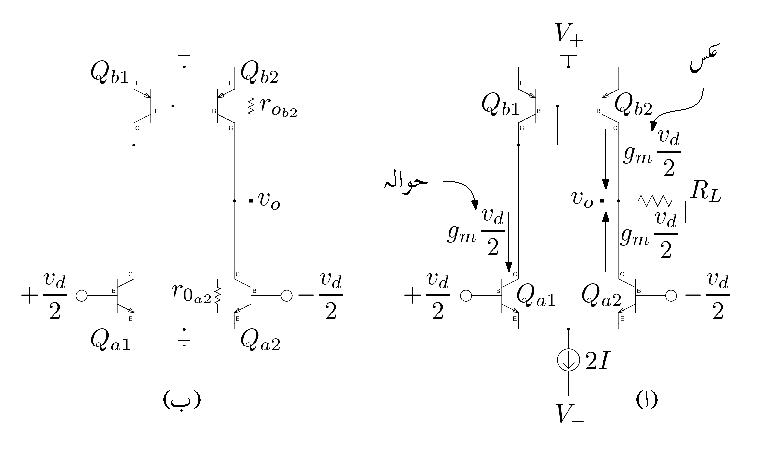
\includegraphics[scale=0.90]{activeLoadedDifferencePair}
\caption{ٹرانزسٹر بوجھ سے لدا دو جوڑ ٹرانزسٹر والا تفرقی ایمپلیفائر}
\label{شکل_ٹرانزسٹر_بار_سے_لدھا_تفرقی_جوڑا}
\end{figure}
اب تصور کریں کہ تفرقی برقی اشارہ \عددی{v_d} مہیا کیا جاتا ہے۔ \عددی{Q_{a1}} اور  \عددی{Q_{a2}} میں بدلتا برقی رو \عددی{g_m \frac{v_d}{2}} پیدا ہو گی جن کی سمتیں شکل میں دکھائی گئی ہیں۔\عددی{Q_{a1}}  کا برقی رو (یعنی \عددی{g_m \frac{v_d}{2}} ) ٹرانزسٹر  \عددی{Q_{b1}} سے بھی گزرتا ہے اور یوں \عددی{Q_{b2}}  اس کا عکس پیدا کرے گا جیسا کہ شکل میں دکھایا گیا ہے۔جوڑ \عددی{v_o} میں دو اطراف سے \عددی{g_m \frac{v_d}{2}}  کی برقی رو داخل ہوتی ہے۔یوں اس جوڑ پر کل داخلی برقی رو کی مقدار \عددی{g_m v_d}  ہے۔ کرخوف کے قانون برائے برقی رو کے مطابق اتنی ہی برقی رو اس جوڑ سے باہر نکلے گی۔یوں بوجھ \عددی{R_L} میں \عددی{g_m v_d} برقی رو زمین کی جانب گزرے گی اور یوں

\begin{align} \label{مساوات_تفرقی_ٹرانزسٹر_سے_لدھے_تفرقی_جوڑے_کا_مخارج}
v_o=\left(g_m \frac{v_d}{2}+g_m \frac{v_d}{2} \right )R_L=g_m R_L v_d
\end{align}
ہو گا اور تفرقی افزائش برقی دباو
\begin{align} \label{مساوات_تفرقی_ٹرانزسٹر_لدھا_تفرقی_افزائش}
A_d=\frac{v_o}{v_d}=g_m R_L
\end{align}
ہو گا۔

مساوات \حوالہ{مساوات_تفرقی_ٹرانزسٹر_سے_لدھے_تفرقی_جوڑے_کا_مخارج}  پر دوبارہ غور کریں۔اس میں \عددی{g_m \frac{v_d}{2}}  ایک مرتبہ تفرقی جوڑے کی وجہ سے اور دوبارہ آئینہ کی وجہ سے ہے۔یوں آئینہ کے دو کردار ہیں۔یہ بطور برقی بوجھ استعمال ہوتا ہے اور ساتھ ہی ساتھ اس کی وجہ سے تفرقی ایمپلیفائر کی افزائش برقی دباو  دگنی ہو جاتی ہے۔

شکل \حوالہ{شکل_ٹرانزسٹر_بار_سے_لدھا_تفرقی_جوڑا} الف میں \عددی{R_L} نہ استعمال کرتے ہوئے اس کی افزائش حاصل کرنے کی خاطر اس کا باریک اشاراتی دور شکل  ب میں دکھایا گیا ہے جہاں ٹرانزسٹر  \عددی{Q_{a2}} اور \عددی{Q_{b2}} کے اندرونی خارجی مزاحمت \عددی{r_o} کو ان کے باہر دکھا کر واضح کیا گیا ہے۔شکل  ب میں ٹرانزسٹر \عددیء{Q_{a1}} اور \عددیء{Q_{a2}} کے ایمٹر کو برقی زمین پر دکھایا گیا ہے۔تفرقی اشارے کے لئے ایسا کرنا ممکن ہے۔اس حقیقت کو مساوات \حوالہ{مساوات_تفرقی_جوڑا_تفرقی_اشارے_کے_لئے_جوڑے_کی_مخارج_برقی_زمین_ہے} میں سمجھایا گیا ہے۔آپ دیکھ سکتے ہیں کہ \عددی{R_L} کی جگہ دونوں ٹرانزسٹروں کے خارجی مزاحمت متوازی جڑے ہیں اور یوں مساوات \حوالہ{مساوات_تفرقی_ٹرانزسٹر_لدھا_تفرقی_افزائش}   کو اس طرح لکھ سکتے ہیں۔
\begin{align} \label{مساوات_تفرقی_ٹرانزسٹر_لدھا_بڑھاتی_الف}
A_d=g_m \left( r_{o_{b2}} \parallel r_{o_{a2}} \right )
\end{align}
اگر \عددی{r_{o_{a2}}} اور \عددی{r_{o_{b2}}} برابر ہوں یعنی  \عددی{r_{o{a2}}=r_{o_{b2}}=r_0}  تب اس مساوات کو مزید سادہ صورت دی جا سکتی ہے یعنی
\begin{align}\label{مساوات_تفرقی_سادہ_ترین_کی_افزائش}
A_d=\frac{g_m r_o}{2}=\frac{1}{2} \left(\frac{I_C}{V_T} \right ) \left(\frac{V_A}{I_C} \right )=\frac{V_A}{2 V_T}
\end{align}
جہاں \عددی{g_m}  کو \عددی{\frac{I_C}{V_T}} اور \عددی{r_o}  کو \عددی{\frac{V_A}{I_C}} لکھا گیا ہے۔

\عددی{V_A=\SI{50}{\volt}} پر یوں 
\begin{align*}
A_d&=\frac{50}{25 \times 10^{-3}}=\SI{2000}{\volt \per \volt}
\end{align*}
حاصل ہو گا۔مساوات \حوالہ{مساوات_تفرقی_ٹرانزسٹر_لدھا_بڑھاتی_الف}  کے مطابق \عددی{r_{o_{a2}}} اور \عددی{r_{o_{b2}}}  کی قیمت بڑھا کر تفرقی ایمپلیفائر کی افزائش مزید بڑھائی جا سکتی ہے۔
%====================
\ابتدا{مثال}
شکل \حوالہ{شکل_تفرقی_حسابی_ایمپلیفائر_بنیادی_دور} میں حسابی ایمپلیفائر کا بنیادی دور دکھایا گیا ہے جہاں تمام ٹرانزسٹر کا \عددی{\beta=100} ہے۔\عددی{Q_1} کا بیس  اور \عددی{Q_4} کا بیس حسابی ایمپلیفائر کے دو داخلی سرے ہیں جنہیں برقی زمین پر رکھا گیا ہے جبکہ \عددی{Q_8} کا ایمٹر حسابی ایمپلیفائر کا خارجی سرا ہے۔
\begin{itemize}
\item
تمام یک سمت متغیرات حاصل کریں۔
\item
داخلی میلان برقی رو \عددیء{I_B} حاصل کریں۔
\end{itemize}

\begin{figure}
\centering
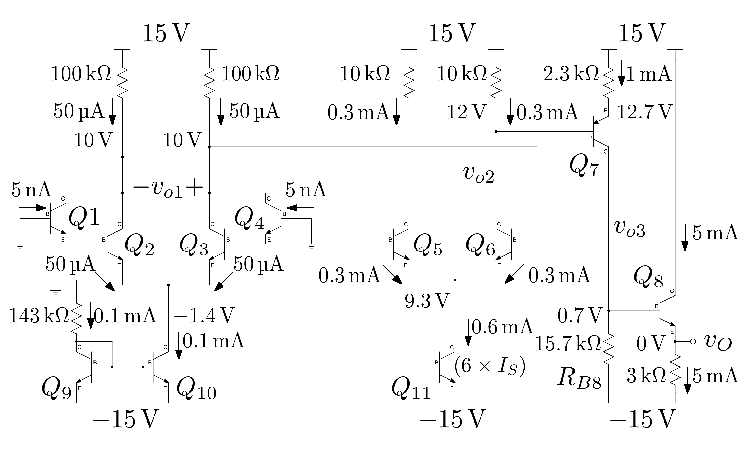
\includegraphics[scale=0.90]{basicOpampInternalCircuit}
\caption{حسابی ایمپلیفائر کا بنیادی دور}
\label{شکل_تفرقی_حسابی_ایمپلیفائر_بنیادی_دور}
\end{figure}

حل:پہلے حسابی ایمپلیفائر کے مختلف حصے پہچانے کی کوشش کرتے ہیں۔\عددیء{Q_9}، \عددیء{Q_{10}} اور \عددیء{\SI{143}{\kilo \ohm}} کا مزاحمت آئینہ برقی رو بناتے ہیں۔\عددیء{Q_{11}} بھی \عددیء{Q_9} کے برقی رو کا عکس پیش کرتا ہے۔\عددیء{Q_1} اور \عددیء{Q_2} مل کر ایک ڈارلنگٹن جوڑی بناتے ہیں۔اسی طرح \عددیء{Q_3} اور \عددیء{Q4} دوسری ڈارلنگٹن جوڑی ہے۔یہ دو ڈارلنگٹن مل کر پہلا یا داخلی تفرقی ایمپلیفائر بناتے ہیں۔\عددیء{Q_5} اور \عددیء{Q_6} دوسرا تفرقی ایمپلیفائر ہے۔\عددیء{Q_7}، \عددیء{\SI{2.3}{\kilo \ohm}} اور \عددیء{\SI{15.7}{\kilo \ohm}} مل کر یک سمت برقی دباو  کی قیمت تبدیل کرتے ہیں جبکہ \عددیء{Q_8} اور \عددی{\SI{3}{\kilo \ohm}} خارجی حصہ ہیں۔

\عددی{Q_9} کے بیس پر
\begin{align*}
V_{B9}=-15+V_{BE}=\SI{-14.3}{\volt}
\end{align*}
ہیں۔اس کے کلکٹر پر بھی یہی برقی دباو ہے لہٰذا اوہم کے قانون سے \عددیء{\SI{143}{\kilo \ohm}} مزاحمت میں
\begin{align*}
\frac{0-(-14.3)}{143000}=\SI{0.1}{\milli \ampere}
\end{align*}
ہے۔\عددی{Q_{10}} کے کلکٹر پر بھی یہی برقی رو پایا جائے گا جبکہ \عددیء{Q_{11}} کے کلکٹر پر چھ گنا زیادہ برقی رو یعنی \عددیء{\SI{0.6}{\milli \ampere}} پایا جائے گا۔

پہلی تفرقی جوڑی میں  \عددیء{\SI{0.1}{\milli \ampere}} برابر تقسیم ہو گا۔یوں \عددی{Q_2} اور \عددی{Q_3} دونوں کا \عددیء{I_C \approx I_E=\SI{50}{\micro \ampere}} ہو گا جبکہ ان کے بیس پر \عددیء{\tfrac{\SI{50}{\micro \ampere}}{\beta}} یعنی \عددیء{\SI{0.5}{\micro \ampere}} پایا جائے گا۔اگر پہلی تفرقی جوڑی میں ڈارلنگٹن استعمال نہ کیا جاتا تب حسابی ایمپلیفائر کا داخلی میلان برقی رو بھی \عددیء{\SI{0.5}{\micro \ampere}} ہی ہوتا۔\عددیء{Q_2} کا بیس برقی رو \عددی{Q_1} کا \عددیء{I_E}۔اسی طرح \عددیء{Q_3} کا بیس برقی رو \عددیء{Q_4} کا \عددیء{I_E} ہے۔یوں \عددیء{Q_1} اور \عددیء{Q_4} کا بیس برقی رو \عددیء{\tfrac{\SI{0.5}{\micro \ampere}}{\beta}} یعنی \عددیء{\SI{5}{\nano \ampere}} ہے۔یوں ڈارلنگٹن کے استعمال سے حسابی ایمپلیفائر کے داخلی میلان برقی رو کو \عددیء{\SI{0.5}{\micro \ampere}} سے کم کرتے ہوئے \عددیء{\SI{5}{\nano \ampere}} کر دیا گیا۔\عددیء{Q_2} کے کلکٹر پر
\begin{align*}
V_{C2}=15-I_{C2} R_{C2}=15 - 50 \times 10^{-6} \times 100 \times 10^{3}=\SI{10}{\volt}
\end{align*}   
پایا جائے گا۔اسی طرح \عددی{Q_3} کے کلکٹر پر بھی \عددیء{\SI{10}{\volt}} پایا جائے گا۔چونکہ \عددیء{Q_1} کا بیس برقی زمین پر ہے لہٰذا \عددیء{V_{B1}=\SI{0}{\volt}} ہے جبکہ اس کا ایمٹر \عددیء{\SI{-0.7}{\volt}} پر ہے۔اس طرح \عددیء{Q_2} کا بیس \عددیء{\SI{-0.7}{\volt}} پر ہے اور یوں اس کا ایمٹر \عددیء{\SI{-1.4}{\volt}} پر ہے۔

\عددیء{Q_5} اور \عددیء{Q_6} پر \عددیء{\SI{0.6}{\milli \ampere}} برابر تقسیم ہو گا۔یوں
\begin{align*}
I_{E5}=I_{E6}=\frac{0.6 \times 10^{-3}}{2}=\SI{0.3}{\milli \ampere}
\end{align*}
پایا جائے گا۔یوں ان کے بیس پر \عددیء{\tfrac{\SI{0.3}{\milli \ampere}}{\beta}} یعنی \عددیء{\SI{3}{\micro \ampere}} پایا جائے گا۔حقیقت میں \عددیء{\SI{3}{\micro \ampere}} اور \عددیء{\SI{50}{\micro \ampere}} مل کر \عددیء{\SI{100}{\kilo \ohm}} سے گزرتے ہیں۔ہم نے پہلی تفرقی جوڑی میں \عددیء{\SI{3}{\micro \ampere}} کو نظر انداز کیا تھا۔اگر اس کو بھی شامل کیا جائے تب پہلی جوڑی کے کلکٹر پر \عددیء{\SI{9.7}{\volt}} پایا جائے گا۔قلم و کاغذ پر جلد حساب کتاب کرتے وقت عموماً اسی طرح بیس پر پائے جانے والے برقی رو کو نظر انداز کیا جاتا ہے۔ہم اسی لئے اس کو نظر انداز کرتے ہوئے \عددیء{\SI{10}{\volt}} کے جواب کو ہی صحیح تسلیم کرتے ہوئے آگے بڑھتے ہیں۔اس طرح \عددیء{Q_5} اور \عددیء{Q_6} کے ایمٹر پر
\begin{align*}
V_{E}=V_{B}-V_{BE}=10-0.7=\SI{9.3}{\volt}
\end{align*}
پایا جائے گا جبکہ ان کے کلکٹر پر 
\begin{align*}
V_{C}=15 -0.3 \times 10^{-3} \times 10000=\SI{12}{\volt}
\end{align*}
پایا جاتا ہے۔یوں \عددیء{V_{CE5}=V_{CE6}=\SI{2.7}{\volt}} ہے اور دونوں ٹرانزسٹر افزائندہ ہیں۔

چونکہ حسابی ایمپلیفائر کے دونوں داخلی سرے برقی زمین پر ہیں لہٰذا ہم توقع کرتے ہیں کہ یہ صفر وولٹ خارج کرے گا۔یہاں ہم دیکھ رہے ہیں کہ دوسرا  تفرقی ایمپلیفائر \عددیء{\SI{12}{\volt}} خارج کر رہا ہے۔یہ ضروری ہے کہ کسی طرح اس برقی دباو سے چٹکارہ حاصل کیا جائے۔\عددیء{Q_7}، \عددیء{\SI{5.3}{\kilo \ohm}} اور \عددیء{\SI{15.7}{\kilo \ohm}} یہی حاصل کرنے میں مدد کرتے ہیں۔\عددیء{Q_7} کے بیس پر \عددیء{\SI{12}{\volt}} ہونے کی وجہ سے اس کے ایمٹر پر 
\begin{align*}
V_{E7}=V_{B7}+V_{EB7}=12+0.7=\SI{12.7}{\volt}
\end{align*}
ہوں گے۔یوں اوہم کے قانون کی مدد سے \عددیء{\SI{2.3}{\kilo \ohm}} میں
\begin{align*}
\frac{15-12.7}{2300}=\SI{1}{\milli \ampere}
\end{align*}
ہو گا جو \عددیء{\SI{15.7}{\kilo \ohm}} سے گزرتے ہوئے اس پر
\begin{align*}
10^{-3} \times 15700=\SI{15.7}{\volt}
\end{align*}
کا برقی دباو پیدا کرے گا جس کی وجہ سے \عددیء{Q_8} کے بیس پر
\begin{align*}
V_{B8}=-15+15.7=\SI{0.7}{\volt}
\end{align*}
پایا جائے گا۔اس طرح \عددیء{Q_8} کے ایمٹر پر
\begin{align*}
V_{E8}=V_{B8}-V_{BE}=0.7-0.7=\SI{0}{\volt}
\end{align*}
پایا جائے گا۔آپ دیکھ سکتے ہیں کہ \عددیء{\SI{2.3}{\kilo \ohm}} اور \عددیء{\SI{15.7}{\kilo \ohm}} کی قیمتوں سے \عددیء{v_O=\SI{0}{\volt}} حاصل کیا گیا۔\عددیء{Q_7} اور اس کے ساتھ منسلک دو مزاحمت یک سمت برقی دباو کی سطح تبدیل کرنے کی صلاحیت رکھتے ہیں۔اسی وجہ سے اس دور کو ہم \اصطلاح {سطح تبدیل کار}\فرہنگ{سطح تبدیل کار}\حاشیہب{level shifter}\فرہنگ{level shifter} کہیں گے۔
\انتہا{مثال}
%================
\ابتدا{مثال}\شناخت{مثال_تفرقی_ڈارلنگٹن_تفرقی_کی_افزائش_برقی_دباو}
شکل \حوالہ{شکل_تفرقی_حسابی_ایمپلیفائر_بنیادی_دور} کے حسابی ایمپلیفائر کو داخلی اشارہ \عددیء{v_d} مہیا کیا جاتا ہے۔ایمپلیفائر کا باریک اشاراتی افزائش \عددیء{A_d=\tfrac{v_O}{v_d}}، داخلی مزاحمت اور خارجی مزاحمت حاصل کریں۔
\begin{figure}
\centering
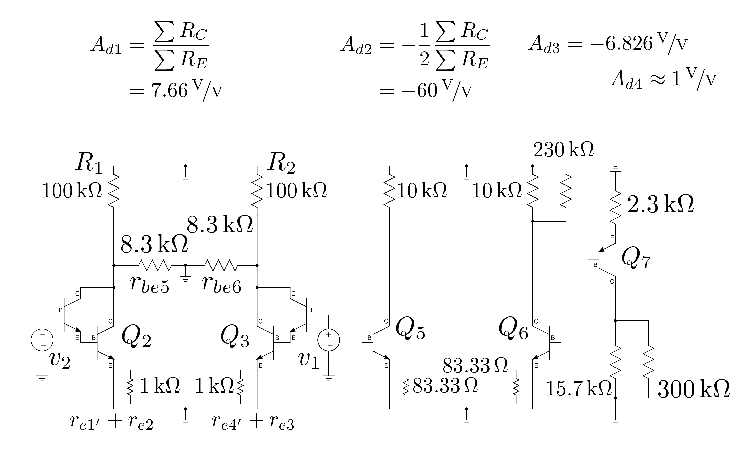
\includegraphics[scale=0.90]{basicOpampInternalCircuitACanalysis}
\caption{}
\label{شکل_تفرقی_حسابی_ایمپلیفائر_دور_بدلتا_مساوی_دور}
\end{figure}

حل:شکل \حوالہ{شکل_تفرقی_حسابی_ایمپلیفائر_دور_بدلتا_مساوی_دور} میں بدلتا رو مساوی دور دکھایا گیا ہے جہاں
\begin{align*}
v_2&=+\frac{v_d}{2}\\
v_1&=-\frac{v_d}{2}
\end{align*}
ہیں۔\عددیء{Q_2} اور \عددیء{Q_3}  میں \عددیء{\SI{50}{\micro \ampere}} برقی رو پایا جاتا ہے لہٰذا ان کے
\begin{align*}
g_{m2}&=g_{m3}=\frac{I_C}{V_T}=\frac{50 \times 10^{-6}}{25 \times 10^{-3}}=\SI{2}{\milli \siemens}\\
r_{e2}&=r_{e3} = \frac{1}{g_m}=\frac{1}{0.002}=\SI{500}{\ohm}
\end{align*}
ہیں۔\عددیء{Q_1} اور \عددیء{Q_4} میں \عددیء{\SI{0.5}{\micro \ampere}} برقی رو پائی جاتی ہے لہٰذا ان کے
\begin{align*}
g_{m1}&=g_{m4}=\frac{0.5 \times 10^{-6}}{25 \times 10^{-3}}=\SI{20}{\micro \siemens}\\
r_{e1}&=r_{e4}=\frac{1}{\SI{20}{\micro \siemens}}=\SI{50}{\kilo \ohm}
\end{align*}
ہیں۔\عددیء{Q_1} کا \عددیء{r_{e1}} چونکہ \عددیء{Q_2} کے بیس پر پایا جاتا ہے لہٰذا اس کو بھی \عددیء{Q_2}  کے ایمٹر پر منتقل کرنا ضروری ہے۔\عددیء{\SI{50}{\kilo \ohm}} منتقل کرنے سے \عددیء{\tfrac{\SI{50}{\kilo \ohm}}{\beta}=\SI{500}{\ohm}} حاصل ہوتا ہے۔یوں \عددیء{r_{e1}} کا عکس \عددیء{r_{e1'}=\SI{500}{\ohm}} حاصل ہوتا ہے۔اس طرح \عددیء{Q_2}  کے ایمٹر پر کل مزاحمت \عددیء{r_{e2}+r_{e1'}} یعنی \عددیء{\SI{1}{\kilo \ohm}}  پایا جائے گا۔اسی طرح \عددیء{Q_4} کا \عددیء{r_{e4}} چونکہ \عددیء{Q_3} کے بیس پر پایا جاتا ہے لہٰذا اس کو بھی \عددیء{Q_3}  کے ایمٹر پر منتقل کرنا ضروری ہے۔\عددیء{\SI{50}{\kilo \ohm}} منتقل کرنے سے \عددیء{\tfrac{\SI{50}{\kilo \ohm}}{\beta}=\SI{500}{\ohm}} حاصل ہوتا ہے۔اس طرح \عددیء{Q_3}  کے ایمٹر پر کل مزاحمت \عددیء{r_{e3}+r_{e4'}} یعنی \عددیء{\SI{1}{\kilo \ohm}}  پایا جائے گا۔ان معلومات کو شکل \حوالہ{شکل_تفرقی_حسابی_ایمپلیفائر_دور_بدلتا_مساوی_دور} پر پیش کیا گیا ہے۔

دوسری تفرقی جوڑی کے \عددیء{Q_5} اور \عددیء{Q_6} میں \عددیء{\SI{0.3}{\milli \ampere}} پایا جاتا ہے لہٰذا ان کے
\begin{align*}
g_{m5}&=g_{m6}=\frac{0.3 \times 10^{-3}}{25 \times 10^{-3}}=\SI{0.012}{\siemens}\\
r_{e5}&=r_{e6}=\frac{1}{0.012}=\SI{83.33}{\ohm}\\
r_{be5}&=r_{be6}=\beta r_e =\SI{8.3}{\kilo \ohm}
\end{align*}
ہیں۔اس جوڑی کا داخلی مزاحمت \عددیء{2 r_{be}} ہے جو پہلی تفرقی جوڑی کا بوجھ بنتا ہے۔شکل میں \عددیء{Q_2} اور \عددیء{Q_3} کے کلکٹر کے مابین \عددیء{\SI{8.3}{\kilo \ohm}} کے سلسلہ وار مزاحمت اسی داخلی مزاحمت کو ظاہر کرتا ہے۔تفرقی اشارے کی صورت میں دوسری تفرقی جوڑی کا ایمٹر برقی زمین پر رہتا ہے۔یوں \عددیء{Q_2} اور \عددیء{Q_3} کے کلکٹر پر دونوں  \عددیء{\SI{8.3}{\kilo \ohm}} کا درمیانی نقطہ برقی زمین پر ہو گا۔ان معلومات کو استعمال کرتے ہوئے آپ دیکھ سکتے ہیں کہ پہلی تفرقی جوڑی کی افزائش
\begin{gather}
\begin{aligned}\label{مساوات_تفرقی_پہلی_کڑی_کی_افزائش}
A_{d1}&=\frac{v_{o1}}{v_d}=\frac{\sum R_C}{\sum R_E}\\
&=\frac{15328}{2000}\\
&=\SI{7.66}{\volt \per \volt}
\end{aligned}
\end{gather} 
حاصل ہوتی ہے جہاں \عددیء{\sum R_C} دونوں ٹرانزسٹر کے کلکٹر پر متوازی جڑے \عددیء{\SI{200}{\kilo \ohm}} اور \عددیء{\SI{16.6}{\kilo \ohm}} کا مجموعی مزاحمت ہے جبکہ \عددیء{\sum R_E} ان کے ایمٹر کے درمیان کُل مزاحمت یعنی \عددیء{2 r_e} ہے۔مثبت افزائش کا مطلب ہے کہ مثبت \عددیء{v_d} کی صورت میں \عددیء{v_{o1}} بھی مثبت ہو گا۔

تیسرے ایمپلیفائر کا داخلی مزاحمت \عددیء{\beta R_{E7}=\SI{230}{\kilo \ohm}} ہے جو \عددیء{R_{C6}} کے متوازی جڑا ہے۔چونکہ
 \عددیء{\SI{230}{\kilo \ohm} \gg \SI{10}{\kilo \ohm}} ہوتا ہے لہٰذا ان کے کُل مزاحمت کو ہم \عددیء{\SI{10}{\kilo \ohm}} ہی لے سکتے ہیں۔اس کا مطلب ہے کہ تیسرے ایمپلیفائر کا داخلی مزاحمت اتنا زیادہ ہے کہ اس کے اثر کو نظرانداز کیا جا سکتا ہے۔یوں دوسرے ایمپلیفائر کی تفرقی افزائش
\begin{align*}
A_{d}&=\frac{\sum R_C}{\sum R_E}\\
&=-\frac{10000}{83.33}\\
&=\SI{-120}{\volt \per \volt}
\end{align*}
ہو گی۔البتہ دوسرے تفرقی جوڑی سے تفرقی اشارہ حاصل نہیں کیا جاتا بلکہ اس کے صرف ایک بازو سے خارجی اشارہ حاصل کیا گیا ہے۔یوں کارآمد افزائش اس قیمت کے آدھی ہو گی یعنی
\begin{gather}
\begin{aligned}\label{مساوات_تفرقی_دوسری_کڑی_کی_افزائش}
A_{d2}&=-\frac{1}{2} \frac{\sum R_C}{\sum R_E}\\
&=-\frac{1}{2}\frac{10000}{83.33}\\
&=\SI{-60}{\volt \per \volt}
\end{aligned}
\end{gather}
افزائش میں منفی کا نشان  یہ دکھلاتا ہے کہ مثبت \عددیء{v_2} اور منفی \عددیء{v_1} کی صورت میں اس حصے کا خارجی اشارہ منفی ہو گا۔

\عددیء{Q_7} اور اس کے ساتھ منسلک \عددی{\SI{2.3}{\kilo \ohm}} اور \عددیء{\SI{15.7}{\kilo \ohm}} مل کر مشترک ایمٹر ایمپلیفائر ہیں۔\عددیء{Q_7} کے \عددیء{r_e} اور \عددیء{Q_8} کے داخلی مزاحمت کو نظر انداز کرتے ہوئے اس ایمپلیفائر کی افزائش
\begin{align*}
A_{d3}=-\frac{15700}{2300}=\SI{-6.826}{\volt \per \volt}
\end{align*}
حاصل ہوتی ہے۔

\عددیء{Q_8} اور اس کے ساتھ منسلک \عددیء{\SI{3}{\kilo \ohm}} مل کر مشترک کلکٹر ایمپلیفائر بناتے ہیں۔مشترک کلکٹر کی افزائش تقریباً ایک کے برابر ہوتی ہے یوں
\begin{align*}
A_{d4} \approx \SI{1}{\volt \per \volt}
\end{align*}
ہو گا۔

ان چاروں افزائش کو استعمال کرتے ہوئے حسابی ایمپلیفائر کی کل افزائش
\begin{align*}
A_d=\frac{v_O}{v_d}&=A_{d1} \times A_{d2} \times  A_{d3} \times A_{d4}\\
&=7.66 \times \left(-60\right) \times \left(-6.826 \right) \times 1\\
&=\SI{3137}{\volt \per \volt}
\end{align*}
حاصل ہوتی ہے۔

شکل  \حوالہ{شکل_تفرقی_حسابی_ایمپلیفائر_دور_بدلتا_مساوی_دور} کو دیکھتے ہوئے \عددیء{Q_2} اور \عددیء{Q_3} کے ایمٹر پر  مزاحمت \عددیء{Q_1} اور \عددیء{Q_4} کے بیس جانب
\begin{align*}
R_i & \approx \left(1000+1000 \right) \times \beta^2\\
&=2000 \times 10000\\
&=\SI{20}{\mega \ohm}
\end{align*}
نظر آئے گا۔یہی حسابی ایمپلیفائر کا داخلی مزاحمت ہے۔

خارجی جانب \عددیء{Q_8} کے \عددیء{r_e} کو نظر انداز کرتے ہیں۔\عددیء{\SI{15.7}{\kilo \ohm}} کا عکس ٹرانزسٹر کے ایمٹر جانب 
\begin{align*}
\frac{15700}{100}=\SI{157}{\ohm}
\end{align*}
نظر آتا ہے۔یہ عکس \عددیء{\SI{3}{\kilo \ohm}} کے متوازی جڑا ہے لہٰذا حسابی ایمپلیفائر کا خارجی مزاحمت
\begin{align*}
R_o=\frac{157 \times 3000}{157+3000} =\SI{149}{\ohm}
\end{align*}
حاصل ہوتا ہے۔

\انتہا{مثال}
%=================
\ابتدا{مثال}\شناخت{مثال_تفرقی_زنجیری_تفرقی_ایمپلیفائر_کی_افزائش}
شکل \حوالہ{شکل_تفرقی_حسابی_ایمپلیفائر_بنیادی_دور} کے حسابی ایمپلیفائر کی افزائش \عددیء{A_i=\tfrac{i_{L}}{i_{b}}} کی مساوات حاصل کریں۔\عددیء{A_i} کو استعمال کرتے ہوئے \عددیء{A_d=\tfrac{v_L}{v_d}} کی مساوات بھی حاصل کریں۔

\begin{figure}
\centering
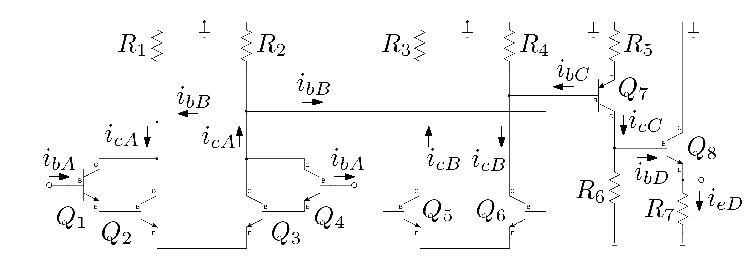
\includegraphics[scale=0.90]{basicOpampInternalCircuitCurrentAnalysis}
\caption{برقی رو کی افزائش}
\label{شکل_تفرقی_حسابی_برقی_رو_افزائش}
\end{figure}
حل:شکل \حوالہ{شکل_تفرقی_حسابی_برقی_رو_افزائش} میں مساوی باریک اشاراتی دور دکھایا گیا ہے جہاں داخلی جانب سے پہلے ایمپلیفائر کو \تحریر{A}، دوسرے کو تحریر{B}، تیسرے کو \تحریر{C} اور خارجی ایمپلیفائر کو \تحریر{D} سے ظاہر کرتے ہوئے زنجیری ضرب سے ہم لکھ سکتے ہیں
\begin{align}\label{مساوات_تفرقی_ڈارلنگٹن_افزائش_رو_کی_بنیادی_زنجیری_مساوات}
A_i=\frac{i_L}{i_b}=\frac{i_{eD}}{i_{bA}}=\frac{i_{eD}}{i_{bD}} \times \frac{i_{bD}}{i_{cC}} \times \frac{i_{cC}}{i_{bC}} \times \frac{i_{bC}}{i_{cB}} \times \frac{i_{cB}}{i_{bB}} \times \frac{i_{bB}}{i_{cA}} \times \frac{i_{cA}}{i_{bA}}
\end{align}
شکل \حوالہ{شکل_تفرقی_حسابی_برقی_رو_افزائش_الف} میں چاروں ایمپلیفائروں کو علیحدہ علیحدہ کیا گیا ہے۔آپ دیکھ سکتے ہیں کہ پہلے ایمپلیفائر کے خارجی جانب دوسرے ایمپلیفائر کا داخلی مزاحمت \عددیء{R_{iB}} نسب ہے۔\عددیء{i_{cA}} کا وہ حصہ جو \عددیء{R_{iB}} سے گزرے درحقیقت دوسرے ایمپلیفائر کا داخلی برقی رو \عددیء{i_{bB}} ہے۔شکل پر اس بات کی وضاحت کی گئی ہے۔یوں اس شکل سے ہم لکھ سکتے ہیں۔ 
\begin{gather}
\begin{aligned}\label{مساوت_تفرقی_ڈارلنگٹن_تمام_کسر}
\frac{i_{eD}}{i_{bD}}&=\beta_8+1\\
\frac{i_{bD}}{i_{cC}}&=\frac{R_6}{R_6+R_{iD}}\\
\frac{i_{cC}}{i_{bC}}&=\beta_7\\
\frac{i_{bC}}{i_{cB}}&=\frac{R_4}{R_4+R_{iC}}\\
\frac{i_{cB}}{i_{bB}}&=\beta_6\\
\frac{i_{bB}}{i_{cA}}&=\frac{R_1+R_2}{R_1+R_2+R_{iB}}\\
\frac{i_{cA}}{i_{bA}}&= \beta_1 \beta_2
\end{aligned}
\end{gather}
%
\begin{figure}
\centering
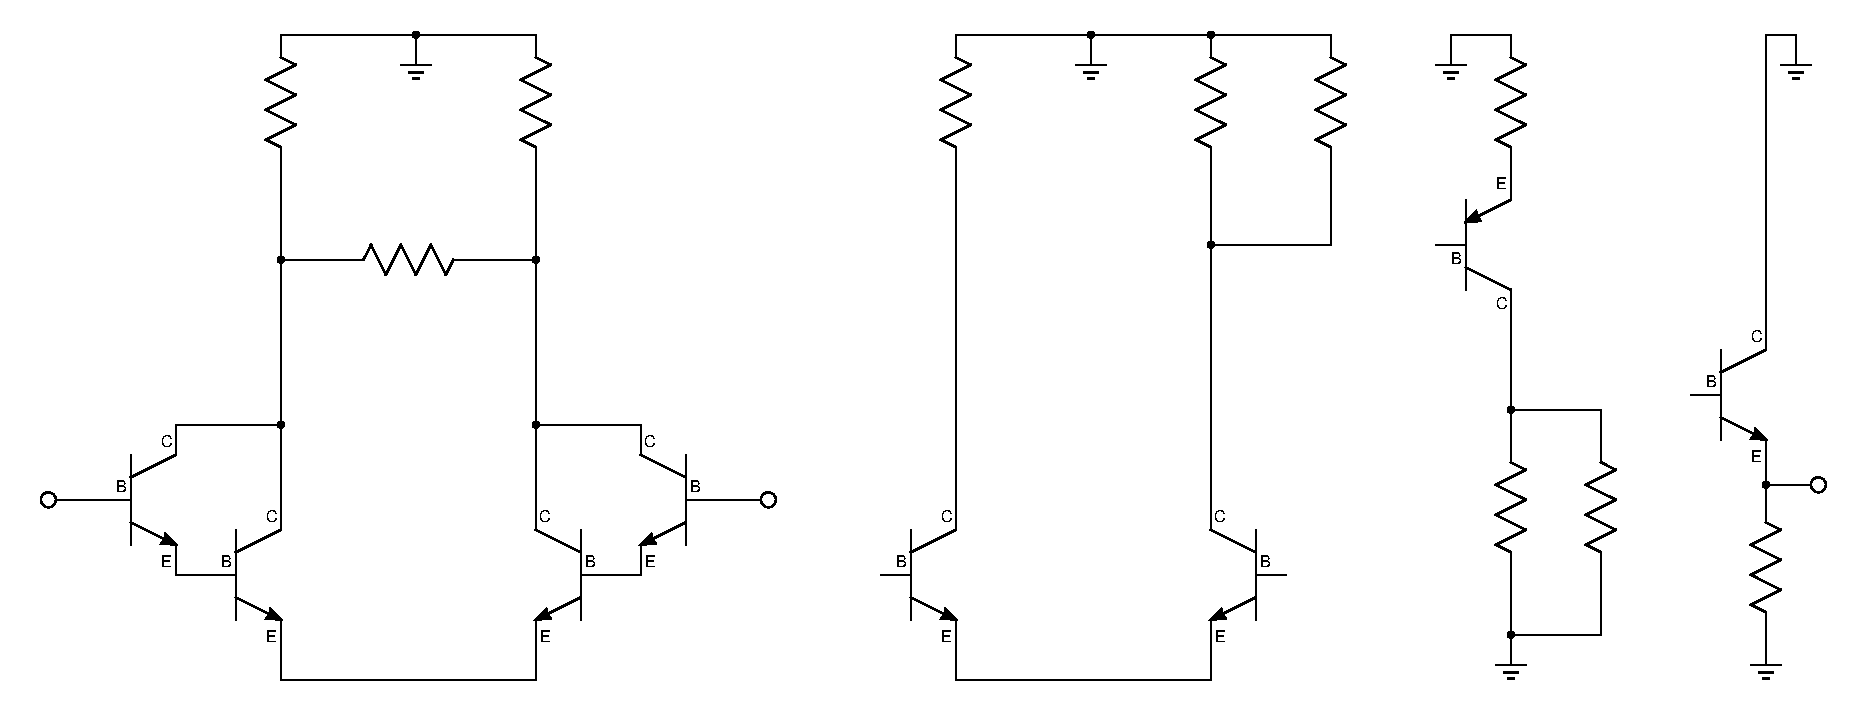
\includegraphics[scale=0.90]{basicOpampInternalCircuitCurrentAnalysisSectioned}
\caption{}
\label{شکل_تفرقی_حسابی_برقی_رو_افزائش_الف}
\end{figure}
تمام ٹرانزسٹر کے \عددیء{\beta} برابر لیتے ہوئے
\begin{gather}
\begin{aligned}
r_{e2}=r_{e3}&=\frac{V_T}{I}\\
r_{be2}=r_{be3}&=\left(\beta+1 \right) r_{e2}\\
r_{e1}=r_{e4}&=\left(\beta+1 \right) \frac{V_T}{I} =\left(\beta+1 \right)r_{e2}\\
r_{be1}=r_{be4}&=\left(\beta+1 \right)^2 r_{e2}
\end{aligned}
\end{gather}
حاصل ہوتے ہیں۔شکل کو دیکھتے ہوئے
\begin{gather}
\begin{aligned}\label{مساوات_تفرقی_ڈارلنگٹن_داخلی_مزاحمتیں}
R_{iA}& =r_{be1}+r_{be4}+\left(r_{be2} +r_{be3}\right) \times \left(\beta +1 \right)\\
&=4 \left(\beta+1 \right)^2 r_{e2}\\
R_{iB}&=2 r_{be5}\\
R_{iC}& \approx R_5 \times \left(\beta+1 \right )\\
R_{iD}& \approx R_7 \times \left(\beta+1 \right) 
\end{aligned}
\end{gather}
لکھا جا سکتا ہے۔مزید یہ کہ
\begin{align*}
v_L&=i_{eD} R_7\\
v_d&=i_{bA} R_{iA}
\end{align*}
لکھتے ہوئے
\begin{gather}
\begin{aligned}\label{مساوات_تفرقی_ڈارلنگٹن_افزائش_برقی_رو_کا_افزائش_رو_سے_حصول}
A_d&=\frac{v_L}{v_d}\\
&=\frac{i_{eD} R_7}{i_{bA} R_{iA}}\\
&=A_i \times \frac{R_7}{R_{iA}}
\end{aligned}
\end{gather}
حاصل ہوتا ہے۔

ذرا کوشش کرنے سے مندرجہ بالا تمام مساوات شکل \حوالہ{شکل_تفرقی_حسابی_ایمپلیفائر_بنیادی_دور} کو دیکھ کر ہی لکھے جا سکتے ہیں۔آپ داخلی جانب یا خارجی جانب  سے شروع ہوتے ہوئے زنجیری ضرب لکھتے ہیں اور پھر زنجیری ضرب کے تمام اجزاء شکل کو دیکھتے ہوئے پُر کرتے ہیں۔
\انتہا{مثال}
%==================
\ابتدا{مثال}
مثال \حوالہ{مثال_تفرقی_زنجیری_تفرقی_ایمپلیفائر_کی_افزائش} میں \عددیء{A_i} اور \عددیء{A_d} کی قیمتیں حاصل کریں۔

حل:مثال \حوالہ{مثال_تفرقی_ڈارلنگٹن_تفرقی_کی_افزائش_برقی_دباو} میں مندرجہ ذیل معلومات حاصل کی گئیں۔
\begin{align*}
r_{e2}&=\SI{500}{\ohm}, \hspace{5mm} r_{e5}=\SI{83.333}{\ohm}
\end{align*}
یوں مساوات \حوالہ{مساوات_تفرقی_ڈارلنگٹن_داخلی_مزاحمتیں} سے
\begin{align*}
R_{iA}&=4 \times 100^2 \times 500=\SI{20}{\mega \ohm}\\
R_{iB}&=2 \times 100 \times 83.333=\SI{1667}{\ohm}\\
R_{iC}& =2300 \times 100=\SI{230}{\kilo \ohm}\\
R_{iD}& =3000 \times 100=\SI{300}{\kilo \ohm}
\end{align*}
اور مساوات \حوالہ{مساوت_تفرقی_ڈارلنگٹن_تمام_کسر} سے 
\begin{align*}
\frac{i_{eD}}{i_{bD}}&=100\\
\frac{i_{bD}}{i_{cC}}&=\frac{15.7 \times 10^3}{15.7 \times 10^3+300 \times 10^3}=0.04973\\
\frac{i_{cC}}{i_{bC}}&=100\\
\frac{i_{bC}}{i_{cB}}&=\frac{10 \times 10^3}{10 \times 10^3+230 \times 10^3}=0.04167\\
\frac{i_{cB}}{i_{bB}}&=100\\
\frac{i_{bB}}{i_{cA}}&=\frac{2 \times 100 \times 10^3}{2 \times 100 \times 10^3+1667}=0.99173\\
\frac{i_{cA}}{i_{bA}}&= 100 \times 100=10000
\end{align*}
حاصل ہوتے ہیں۔اس طرح مساوات \حوالہ{مساوات_تفرقی_ڈارلنگٹن_افزائش_رو_کی_بنیادی_زنجیری_مساوات} سے 
\begin{align*}
A_i=\frac{i_{eD}}{i_{bA}}&=100 \times 0.04973 \times 100 \times 0.04167 \times 100 \times 0.99173 \times 10000\\
&=\SI{20.55}{\mega \ampere \per \ampere}
\end{align*}
اور مساوات \حوالہ{مساوات_تفرقی_ڈارلنگٹن_افزائش_برقی_رو_کا_افزائش_رو_سے_حصول} سے 
\begin{align*}
A_d=\frac{v_L}{v_d} &=20.55 \times 10^6 \times \frac{3000}{20 \times 10^6}\\
&=\SI{3082}{\volt \per \volt}
\end{align*}
حاصل ہوتا ہے۔مثال \حوالہ{مثال_تفرقی_ڈارلنگٹن_تفرقی_کی_افزائش_برقی_دباو} میں \عددیء{A_d=\SI{3137}{\volt \per \volt}} حاصل کی گئی۔دونوں جوابات میں فرق \عددیء{\alpha \approx 1} اور اس طرح کے دیگر استعمال کئے گئے قیمتوں میں معمولی معمولی فرق کی وجہ سے ہے۔ان دو جوابات میں صرف
\begin{align*}
\abs{\frac{3137-3082}{3137}} \times 100=\SI{1.75}{\percent}
\end{align*}
کا فرق ہے۔
\انتہا{مثال}
%===================

شکل \حوالہ{شکل_تفرقی_حسابی_ایمپلیفائر_دور_بدلتا_مساوی_دور} میں دوسرے ایمپلیفائر کا داخلی مزاحمت \عددیء{r_{be5}+r_{be6}=\SI{16.6}{\kilo \ohm}} ہے جو پہلی ایمپلیفائر کا بوجھ بنتا ہے۔یوں \عددیء{r_{be5}+r_{be6}} اور \عددیء{R_1+R_2} متوازی جڑے نظر آتے ہیں۔چونکہ \عددیء{r_{be5}+r_{be6} \ll R_1+R_2} ہے لہٰذا ان متوازی جڑے مزاحمت کے مجموعی مزاحمت کو تقریباً  \عددیء{r_{be5}+r_{be6}} لیا جا سکتا ہے۔اس کے برعکس تیسرے ایمپلیفائر کا داخلی مزاحمت بہت بڑا ہے لہٰذا دوسرے ایمپلیفائر پر اس کے بوجھ کو نظرانداز کیا جاتا ہے۔ایسا کرنے سے پہلے اور دوسرے ایمپلیفائر کے افزائش  یوں لکھے جا سکتے ہیں۔
\begin{align*}
A_{d1}&=\frac{\sum R_C}{\sum R_E}=\frac{r_{be5}+r_{be6}}{4 r_{e2}}\\
A_{d2}& \approx -\frac{1}{2}\frac{\sum R_C}{\sum R_E}=-\frac{1}{2} \left(\frac{R_{C6}}{r_{e5}+r_{e6}}\right)
\end{align*}
اس طرح ان دو کڑیوں کی کُل افزائش
\begin{gather}
\begin{aligned}
A_d=A_{d1} A_{d2}&=-\frac{1}{2}  \times \left(\frac{r_{be5}+r_{be6}}{4 r_{e2}}\right) \times \left(\frac{R_{C6}}{r_{e5}+r_{e6}}\right)\\
&=-\frac{1}{2}  \times \frac{\left(\beta+1 \right) \left(r_{e5}+r_{e6}\right)}{4 r_{e2}} \times \left(\frac{R_{C6}}{r_{e5}+r_{e6}}\right)\\
&=-\frac{1}{2}  \times \frac{\left(\beta+1 \right)R_{C6} }{4 r_{e2}}
\end{aligned}
\end{gather}
حاصل ہوتی ہے۔اس مساوات کے تحت \عددیء{\beta}  بڑھانے اور \عددیء{r_{e2}} گھٹانے سے افزائش بڑھتی ہے۔چونکہ \عددیء{r_e =\tfrac{V_T}{I_C}} ہوتا ہے لہٰذا \عددیء{I} بڑھانے سے \عددیء{r_{e2}} گھٹے گا۔

اس کے علاوہ اگر پہلے ایمپلیفائر میں ڈارلنگٹن جوڑی استعمال نہ کی جائے تب اس کی داخلی مزاحمت آدھی اور  افزائش دگنی ہو جائے گی۔

صفحہ \حوالہصفحہ{مساوات_ٹرانزسٹر_داخلی_مزاحمت_بالمقابل_افزائش} پر مساوات \حوالہ{مساوات_ٹرانزسٹر_داخلی_مزاحمت_بالمقابل_افزائش} پر تبصرہ کرتے وقت یہ حقیقت بتلائی گئی تھی کہ اگر افزائش بڑھائی جائے تو داخلی مزاحمت گھٹتی ہے۔تفرقی ایمپلیفائر میں بھی داخلی مزاحمت گھٹاتے ہوئے افزائش بڑھانا ممکن ہے۔
%==================
\حصہ{وائڈلر منبع برقی رو}
شکل \حوالہ{شکل_آئینہ_برقی_رو_الف} میں \عددیء{Q_2} کے ایمٹر پر \عددیء{R_E} نسب کرنے سے  \اصطلاح {وائڈلر منبع برقی رو}\فرہنگ{وائڈلر منبع رو}\فرہنگ{منبع برقی رو!وائڈلر}\حاشیہب{Widlar current source}\فرہنگ{Widlar current source} حاصل ہوتا ہے جسے شکل \حوالہ{شکل_تفرقی_وائڈلر_پیداکار_برقی_رو} میں\حاشیہد{باب وائڈلر نے اس دور کو دریافت کیا۔} میں دکھایا گیا ہے۔ٹرانزسٹر کے برقی رو کے مساوات کو استعمال کرتے ہوئے 
\begin{figure}
\centering
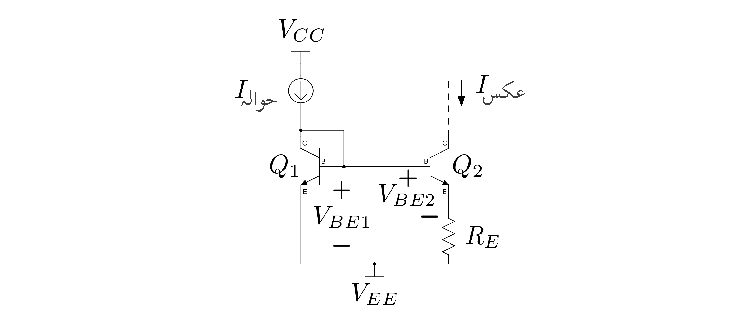
\includegraphics[scale=0.90]{widlarCurrentSource}
\caption{وائڈلر منبع برقی رو}
\label{شکل_تفرقی_وائڈلر_پیداکار_برقی_رو}
\end{figure}
%
\begin{align*}
V_{BE1}&=V_T \ln \left(\frac{I_{\textrm{حوالہ}}}{I_S} \right)\\
V_{BE2}&=V_T \ln \left(\frac{I_{\textrm{عکس}}}{I_S} \right)
\end{align*}
لکھا جا سکتا ہے۔ان دو مساوات کو آپس میں منفی کرنے سے
\begin{align*}
V_{BE1}-V_{BE2}=V_T \ln \left(\frac{I_{\textrm{حوالہ}}}{I_{\textrm{عکس}}} \right)
\end{align*}
حاصل ہوتا ہے۔شکل کو دیکھتے ہوئے ہم 
\begin{align*}
V_{BE1}=V_{BE2}+I_{\textrm{عکس}} R_E
\end{align*}
لکھ سکتے ہیں۔یوں
\begin{align}\label{مساوات_تفرقی_وائڈلر_مزاحمت}
I_{\textrm{عکس}} R_E=V_T \ln \left(\frac{I_{\textrm{حوالہ}}}{I_{\textrm{عکس}}} \right)
\end{align}
لکھا جا سکتا ہے۔

آئیں وائڈلر منبع برقی رو کی خارجی مزاحمت \عددیء{R_o} حاصل کریں۔ایسا کرنے کی خاطر \عددی{Q_2} کے کلکٹر پر \عددیء{v_t} برقی دباو مہیا کرتے ہوئے \عددیء{i_t} کا حساب لگا کر \عددیء{\tfrac{v_t}{i_t}} معلوم کیا جا سکتا ہے جو کہ \عددیء{R_o} کی قیمت ہو گی۔

وائڈلر منبع برقی رو میں \عددیء{Q_1} کے کلکٹر اور بیس آپس میں جڑے ہیں۔یوں یہ بطور ڈایوڈ کردار ادا کرتا ہے۔صفحہ \حوالہصفحہ{مساوات_ٹرانزسٹر_ڈایوڈ_جڑے_ٹرانزسٹر_کی_مزاحمت} پر مساوات \حوالہ{مساوات_ٹرانزسٹر_ڈایوڈ_جڑے_ٹرانزسٹر_کی_مزاحمت} ایسے ٹرانزسٹر کی مزاحمت \عددیء{r_e} دیتا ہے۔وائڈلر منبع رو کی خارجی مزاحمت حاصل کرنے کی خاطر \عددیء{Q_2} کا پائے ریاضی نمونہ استعمال کرتے ہیں جبکہ \عددیء{Q_1} کی جگہ اس کا باریک اشاراتی مساوی مزاحمت \عددیء{r_e} نسب کرتے ہیں۔ایسا کرتے ہوئے شکل \حوالہ{شکل_تفرقی_وائڈلر_پیداکار_برقی_رو_مساوی} الف حاصل ہوتا ہے۔آپ جانتے ہیں کہ \عددیء{r_{be}=r_e\left(\beta+1 \right)} ہوتا ہے۔یوں \عددیء{r_{be}\gg r_e} ہے لہٰذا سلسلہ وار جڑے \عددیء{r_{be}} اور \عددیء{r_e} میں \عددیء{r_e} کو نظرانداز کیا جا سکتا ہے۔ایسا کرنے سے شکل  ب حاصل ہوتا ہے جہاں سے صاف ظاہر ہے کہ \عددیء{R_E} اور \عددیء{r_{be}} متوازی جڑے ہیں۔\عددیء{R_E \mathbin{\|} r_{be}} کو \عددیء{R_E'} لکھتے ہوئے اس میں برقی رو کو \عددیء{\tfrac{v_{be}}{R_E'}} لکھا جا سکتا ہے۔
%
\begin{figure}
\centering
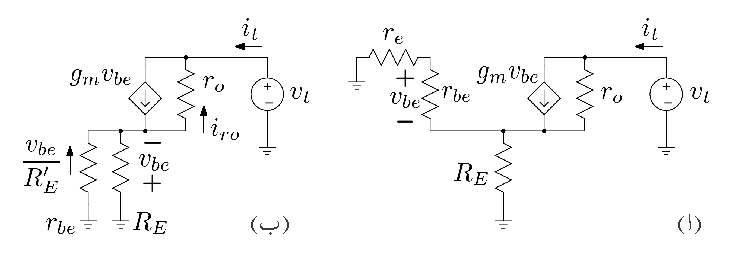
\includegraphics[scale=0.90]{widlarCurrentSourceSmallSignalEquivalent}
\caption{وائڈلر منبع رو کا باریک اشاراتی مساوی دور}
\label{شکل_تفرقی_وائڈلر_پیداکار_برقی_رو_مساوی}
\end{figure}
اس برقی رو کی سمت شکل میں دکھائی گئی ہے۔کرخوف کے قانون برائے برقی رو کی مدد سے
\begin{align*}
g_m v_{be}+\frac{v_{be}}{R_E'}=i_{ro} 
\end{align*}
لکھا جا سکتا ہے جس سے
\begin{align*}
i_{ro}=\left(g_m +\frac{1}{R_E'} \right) v_{be}
\end{align*}
حاصل ہوتا ہے۔یوں کرخوف کے قانون برائے برقی دباو کی مدد سے
\begin{align}\label{مساوات_تفرقی_وائڈلر_ٹیسٹ_برقی_دباو}
v_t=-v_{be}-\left(g_m +\frac{1}{R_E'} \right) v_{be} r_o
\end{align}
اور کرخوف کے قانون برائے برقی رو کی مدد سے
\begin{align}\label{مساوات_تفرقی_وائڈلر_ٹیسٹ_برقی_رو}
i_t=g_m v_{be}-\left(g_m +\frac{1}{R_E'} \right) v_{be}
\end{align}
لکھا جا سکتا ہے۔مساوات \حوالہ{مساوات_تفرقی_وائڈلر_ٹیسٹ_برقی_دباو} کو مساوات \حوالہ{مساوات_تفرقی_وائڈلر_ٹیسٹ_برقی_رو} سے تقسیم کرتے ہوئے وائڈلر منبع کی خارجی مزاحمت \عددیء{R_o} یوں حاصل ہوتی ہے۔
\begin{align*}
R_o=\frac{v_t}{i_t}&=R_E' \left[1+r_o \left(g_m+\frac{1}{R_E'} \right) \right]\\
&=R_E'+r_o\left(1+g_m R_E' \right)
\end{align*}
اس مساوات میں \عددیء{R_E'} کو نظر انداز کرتے ہوئے خارجی مزاحمت \عددیء{R_o} کی سادہ مساوات
\begin{align}\label{مساوات_تفرقی_قابو_زمین_مخارج_مزاحمت_خارجی_مزاحمت}
R_o\approx r_o\left(1+g_m R_E' \right)
\end{align}
حاصل ہوتی ہے جہاں
\begin{align}\label{مساوات_تفرقی_قابو_زمین_مخارج_مزاحمت_خارجی_مزاحمت_الف}
R_E'=\frac{r_{be} R_E}{r_{be}+R_E}
\end{align}
کے برابر ہے۔اس طرح خارجی مزاحمت \عددیء{r_o} سے بڑھ کر \عددیء{r_o \left(1+g_m R_E' \right)} ہو گئی ہے۔یہ ایک عمومی نتیجہ ہے اور یوں کسی بھی دو جوڑ ٹرانزسٹر جس کے ایمٹر پر \عددیء{R_E} مزاحمت نسب ہو اور جس کا بیس سرا برقی زمین پر ہو کی خارجی مزاحمت مساوات \حوالہ{مساوات_تفرقی_قابو_زمین_مخارج_مزاحمت_خارجی_مزاحمت} سے حاصل ہو گی۔
%====================
\ابتدا{مثال}
شکل \حوالہ{شکل_تفرقی_وائڈلر_آئینہ_مثال} میں سادہ آئینہ اور وائڈلر آئینہ دکھائے گئے ہیں۔\عددیء{I_{\textrm{عکس}}=\SI{15}{\micro \ampere}} حاصل کرنے کی خاطر درکار مزاحمت حاصل کریں۔

\begin{figure}
\centering
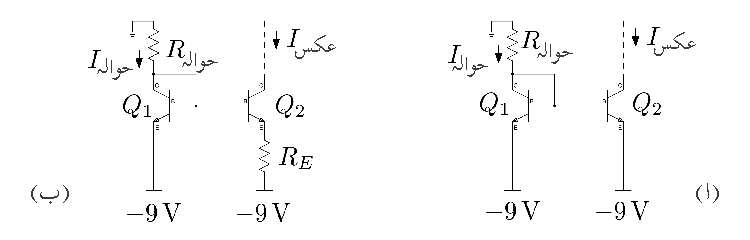
\includegraphics[scale=0.90]{widlarExample}
\caption{ولسن آئینہ}
\label{شکل_تفرقی_وائڈلر_آئینہ_مثال}
\end{figure}

حل:شکل  الف میں \عددیء{\SI{15}{\micro \ampere}} حاصل کرنے کی خاطر
\begin{align*}
R_{\textrm{حوالہ}}=\frac{9-0.7}{15 \times 10^{-6}}=\SI{553}{\kilo \ohm}
\end{align*}
درکار ہے۔شکل  ب میں \عددیء{I_{\textrm{حوالہ}}=\SI{1}{\milli \ampere}} رکھتے ہوئے \عددیء{I_{\textrm{عکس}}=\SI{15}{\micro \ampere}} حاصل کرتے ہیں۔\عددیء{I_{\textrm{حوالہ}}=\SI{1}{\milli \ampere}} حاصل کرنے کی خاطر
\begin{align*}
R_{\textrm{حوالہ}}=\frac{9-0.7}{1 \times 10^{-3}}=\SI{8.3}{\kilo \ohm}
\end{align*}
اور مساوات \حوالہ{مساوات_تفرقی_وائڈلر_مزاحمت} سے
\begin{align*}
R_E=\frac{25 \times 10^{-3}}{15 \times 10^{-6}} \ln \left(\frac{10^{-3}}{15 \times 10^{-6}} \right)=\SI{7}{\kilo \ohm}
\end{align*}
حاصل ہوتے ہیں۔آپ نے دیکھا کہ  کم برقی رو پیدا کرنے کی خاطر سادہ منبع رو کو \عددیء{\SI{553}{\kilo \ohm}} جبکہ وائڈلر منبع رو کو \عددیء{\SI{8.3}{\kilo \ohm}} اور \عددیء{\SI{7}{\kilo \ohm}} کے مزاحمت درکار ہیں۔جیسا کہ آپ جانتے ہیں کہ مخلوط دور میں زیادہ قیمت کا مزاحمت زیادہ جگہ گھیرتا ہے جو کہ مہنگا پڑتا ہے۔اسی لئے مخلوط ادوار میں وائڈلر منبع رو استعمال کیا جائے گا۔
\انتہا{مثال}
%==================
\حصہ{ولسن آئینہ}
شکل \حوالہ{شکل_آئینہ_برقی_رو_الف} میں سادہ آئینہ برقی رو دکھایا گیا۔\عددیء{V_{BE}=\SI{0.7}{\volt}} لیتے ہوئے  \عددیء{V_{CE1}=\SI{0.7}{\volt}} ہے جبکہ  \عددیء{V_{CE2}} پر ایسی کوئی پابندی لاگو نہیں لہٰذا عموماً \عددیء{V_{CE1} \neq V_{CE2}} ہوتا ہے۔اب تک آئینہ برقی رو پر تبصروں میں ہم نے ارلی برقی دباو کے اثرات کو نظرانداز کیا۔حقیقت میں اگرچہ شکل \حوالہ{شکل_آئینہ_برقی_رو_الف} میں \عددیء{V_{BE1}=V_{BE2}} ہے لیکن  \عددیء{V_{CE1} \neq V_{CE2}} کی بنا پر ارلی برقی دباو \عددیء{Q_1} اور \عددیء{Q_2} کے برقی رو میں فرق پیدا کرتا ہے۔\عددیء{V_{CE1}} اور \عددیء{V_{CE2}} میں فرق کو کم کرنے سے ارلی برقی دباو کے اثر کو کم کیا جا سکتا ہے۔اسی غرض سے شکل \حوالہ{شکل_آئینہ_برقی_رو_الف} میں تیسرا ٹرانزسٹر شامل کرتے ہوئے شکل \حوالہ{شکل_تفرقی_ولسن_آئینہ} الف حاصل ہوتا ہے جس کو \اصطلاح {ولسن آئینہ}\فرہنگ{ولسن آئینہ}\فرہنگ{آئینہ!ولسن}\حاشیہب{Wilson mirror} کہتے\حاشیہد{جارج آر ولسن نے اس آئینہ کو دریافت کیا۔} ہیں۔ولسن آئینے میں
\begin{align*}
V_{CE1}&=V_{BE1}=\SI{0.7}{\volt}\\
V_{CE2}&=V_{BE1}+V_{BE3}=\SI{1.4}{\volt}
\end{align*}
ہیں۔دونوں ٹرانزسٹر کے \عددیء{V_{CE}} میں فرق صرف \عددیء{\SI{0.7}{\volt}} رہ گیا ہے۔
\begin{figure}
\centering
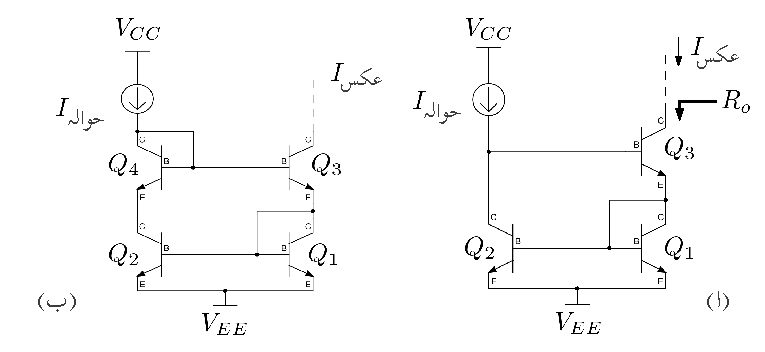
\includegraphics[scale=0.90]{wilsonCurrentMirror}
\caption{ولسن آئینہ}
\label{شکل_تفرقی_ولسن_آئینہ}
\end{figure}
اس دور کو حل کرتے ہوئے تمام ٹرانزسٹر کو بالکل یکساں تصور کیا جائے گا۔چونکہ \عددیء{I_{\textrm{عکس}}} دراصل \عددیء{i_{C3}} ہی ہے لہٰذا ہم \عددیء{i_{C3}} اور \عددیء{I_{\textrm{حوالہ}}} کا تعلق حاصل کریں گے۔\عددیء{Q_1} اور \عددیء{Q_2} کے لئے ہم لکھ سکتے ہیں۔
\begin{align*}
i_{C1}&=i_{C2}=i_C\\
i_{B1}&=i_{B2}=i_B
\end{align*}
\عددیء{Q_3} کے لئے
\begin{gather}\label{مساوات_تفرقی_ولسن_تیسرے_ٹرانزسٹر_رو}
\begin{aligned}
i_{B3}&=\frac{i_{C3}}{\beta}\\
i_{E3}&=\left(\frac{\beta+1}{\beta}\right) i_{C3}
\end{aligned}
\end{gather}
لکھا جا سکتا ہے۔کرخوف کے قانون برائے برقی رو کے تحت
\begin{gather}
\begin{aligned}\label{مساوات_تفرقی_ولسن_کرخوف_کا_قانون}
i_{E3}&=i_{C1}+i_{B1}+i_{B2}\\
&=i_C+2 i_B\\
&=\left(\frac{\beta+2}{\beta} \right) i_C
\end{aligned}
\end{gather}
لکھا جا سکتا ہے۔مندرجہ بالا دو مساوات میں \عددیء{i_{E3}} کو برابر لکھتے ہوئے
\begin{align*}
\left(\frac{\beta+1}{\beta}\right) i_{C3}=\left(\frac{\beta+2}{\beta} \right) i_C
\end{align*}
\عددیء{i_C} کی مساوات حاصل ہوتی ہے۔
\begin{align}\label{مساوات_تفرقی_محاصل_رو_کی_مساوات}
i_C=\left(\frac{\beta+1}{\beta+2}\right) i_{C3}
\end{align}
کرخوف کے قانون برائے برقی رو کی مدد سے 
\begin{align*}
I_{\textrm{حوالہ}}&=i_{C2}+i_{B3}\\
&=i_{C}+\frac{i_{C3}}{\beta}
\end{align*}
لکھا جا سکتا ہے جس میں \عددیء{i_C} کی قیمت مساوت \حوالہ{مساوات_تفرقی_محاصل_رو_کی_مساوات} سے پُر کرتے ہوئے
\begin{align*}
I_{\textrm{حوالہ}}&=\left(\frac{\beta+1}{\beta+2}\right) i_{C3}+\frac{i_{C3}}{\beta}\\
&=\left(\frac{\beta+1}{\beta+2}+\frac{1}{\beta} \right) i_{C3}
\end{align*}
لکھا جا سکتا ہے۔اس مساوات سے
\begin{align*}
I_{\textrm{حوالہ}}&=\left[\frac{\beta \left(\beta+1 \right)+\beta+2}{\beta \left(\beta+2 \right)}\right]i_{C3}\\
&=\left[\frac{\beta^2+2 \beta+2}{\beta \left(\beta+2 \right)}\right]i_{C3}\\
&=\left[\frac{\beta \left(\beta+2 \right)+2}{\beta \left(\beta+2 \right)}\right]i_{C3}
\end{align*}
حاصل ہوتا ہے جسے یوں لکھا جا سکتا ہے۔
\begin{align*}
I_{\textrm{عکس}}=i_{C3}&=\left[\frac{\beta \left(\beta+2 \right)}{\beta \left(\beta+2 \right)+2}\right] I_{\textrm{حوالہ}}\\
&=\left[\frac{1}{1+\frac{2}{\beta \left(\beta+2 \right)}} \right] I_{\textrm{حوالہ}}
\end{align*}
اس مساوات کو 
\begin{align}
I_{\textrm{عکس}} \approx \left[\frac{1}{1+\frac{2}{\beta^2 }} \right] I_{\textrm{حوالہ}}
\end{align}
لکھا جا سکتا ہے۔اس مساوات کا صفحہ \حوالہصفحہ{مساوات_تفرقی_بہتر_آئینہ_کی_مساوات} پر مساوات \حوالہ{مساوات_تفرقی_بہتر_آئینہ_کی_مساوات} کے ساتھ موازنہ کریں۔دونوں مساوات بالکل ایک جیسے ہیں۔
\begin{figure}
\centering
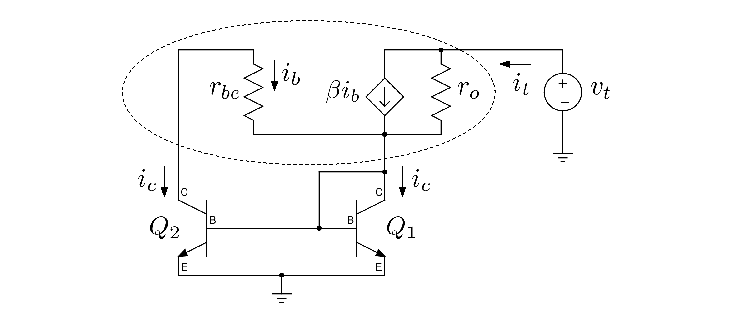
\includegraphics[scale=0.90]{wilsonMirrorOutputImpedance}
\caption{ولسن آئینے کی خارجی مزاحمت}
\label{شکل_تفرقی_ولسن_آئینے_کی_خارجی_مزاحمت}
\end{figure}

آئیں آئینے کی خارجی مزاحمت حاصل کریں۔ایسا کرنے کی خاطر \عددیء{Q_3} کے کلکٹر پر \عددیء{v_t} لاگو کرتے ہوئے \عددیء{i_t} کا حساب لگاتے ہیں۔\عددیء{\tfrac{v_t}{i_t}} خارجی مزاحمت \عددیء{R_o} ہو گا۔\عددیء{Q_3} کا پائے ریاضی نمونہ استعمال کرتے ہوئے ولسن آئینے کو شکل \حوالہ{شکل_تفرقی_ولسن_آئینے_کی_خارجی_مزاحمت} میں دکھایا گیا ہے۔نقطہ دار دائرے سے  دو جگہ \عددیء{i_c} برقی رو خارج اور ایک جگہ \عددیء{i_t} داخلی ہو رہی ہے۔یوں کرخوف کے قانون برائے برقی رو کی مدد سے ہم لکھ سکتے ہیں
\begin{align}\label{مساوات_تفرقی_ولسن_ٹیست_برقی_رو}
i_t=2 i_c
\end{align}

شکل \حوالہ{شکل_تفرقی_ولسن_آئینے_کی_خارجی_مزاحمت} میں \عددیء{Q_1} کا بیس اس کے کلکٹر کے ساتھ جڑا ہے جس  کی وجہ سے یہ بطور ڈایوڈ کردار ادا کرتا ہے اور اس کو مزاحمت \عددیء{r_e} سے ظاہر کیا جا سکتا ہے۔\عددیء{Q_2} کا \عددیء{r_{be}} اس \عددیء{r_e} کے متوازی جڑا ہے۔چونکہ \عددیء{r_e \ll r_{be}} ہوتا ہے لہٰذا ان کا مساوی مزاحمت تقریباً \عددیء{r_e} ہی کے برابر ہو گا۔شکل \حوالہ{شکل_تفرقی_ولسن_آئینے_کی_خارجی_مزاحمت_الف} میں اس حقیقت کو مد نظر رکھتے ہوئے دور کو دوبارہ دکھائی ہے۔\عددیء{Q_1} اور \عددیء{Q_2} کے کلکٹر پر برقرار \عددیء{i_c} برقی رو گزرے گی جسے شکل میں دکھایا گیا ہے۔
\begin{figure}
\centering
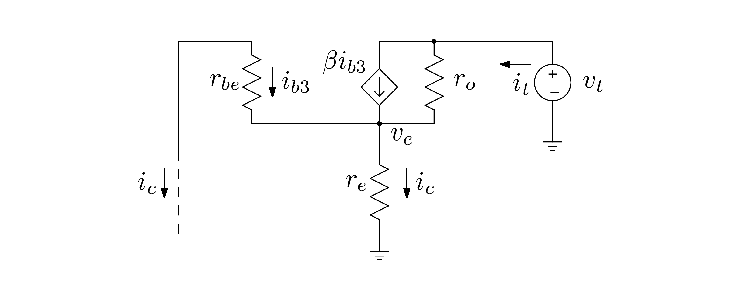
\includegraphics[scale=0.90]{wilsonCurrentMirrorOutputImpedanceA}
\caption{ولسن آئنے کی خارجی مزاحمت}
\label{شکل_تفرقی_ولسن_آئینے_کی_خارجی_مزاحمت_الف}
\end{figure}
شکل کو دیکھتے ہوئے
\begin{align*}
v_e&=i_c r_e\\
i_{b3}&=-i_c
\end{align*}
لکھا جا سکتا ہے۔ساتھ ہی ساتھ کرخوف کے قانون برائے برقی رو کی مدد سے
\begin{align*}
i_t&=\beta i_{b3} +\frac{v_t-v_e}{r_{o3}}\\
&=-\beta i_c +\frac{v_t}{r_{o3}}-\frac{v_e}{r_{o3}}\\
&=-\beta i_c +\frac{v_t}{r_{o3}}-\left(\frac{r_e}{r_{o3}}\right) i_c
\end{align*}
لکھا جا سکتا ہے جہاں دوسرے قدم پر \عددیء{i_{b3}=-i_c} کا استعمال کیا گیا۔چونکہ \عددیء{r_e \ll r_o} ہوتا ہے لہٰذا مندرجہ بالا مساوات میں آخری جزو کو نظرانداز کیا جا سکتا ہے۔یوں مساوات \حوالہ{مساوات_تفرقی_ولسن_ٹیست_برقی_رو} کے استعمال سے 
\begin{align*}
2 i_c=-\beta i_c +\frac{v_t}{r_{o3}}
\end{align*}
حاصل ہوتا ہے جس کو
\begin{align*}
i_c \left(\beta+2 \right) r_{o3}=v_t
\end{align*}
لکھا جا سکتا ہے۔ولسن آئینے کا خارجی مزاحمت \عددیء{R_o=\tfrac{v_t}{i_t}} کے برابر ہے جہاں \عددیء{i_t=2 i_c} ہے۔یوں
\begin{align}
R_o=\frac{v_t}{i_t}=\frac{v_t}{2 i_c}=\frac{\left(\beta+2 \right) r_{o3}}{2}
\end{align}
حاصل ہوتا ہے جس کو
\begin{align} \label{مساوات_تفرقی_ولسن_کی_خارجی_مزاحمت}
R_o \approx \frac{\beta r_{o}}{2}
\end{align}
لکھا جا سکتا ہے جہاں \عددیء{r_{o3}} کو \عددیء{r_o} لکھا گیا ہے۔آپ دیکھ سکتے ہیں کہ ولسن آئینے کی خارجی مزاحمت \عددیء{r_o} سے \عددیء{\tfrac{\beta}{2}} گنا زیادہ ہے۔


اس حصے کے شروع میں ذکر کیا گیا کہ ارلی برقی دباو کے اثر کو کم کرنے کی خاطر ولسن آئینے میں \عددیء{V_{CE1}} اور \عددیء{V_{CE2}} میں فرق کو کم کرتے ہوئے \عددیء{\SI{0.7}{\volt}} کر دیا گیا۔اس فرق کو مکمل طور ختم بھی کیا جا سکتا ہے۔شکل \حوالہ{شکل_تفرقی_ولسن_آئینہ} ب میں \عددیء{Q_4} کی شمولیت سے 
\begin{align*}
V_{CE2}=V_{BE1}+V_{BE3}-V_{BE4}=\SI{0.7}{\volt}
\end{align*}
ہو جاتا ہے۔یوں \عددیء{V_{CE1}=V_{CE2}=\SI{0.7}{\volt}} کرتے  ہوئے ارلی برقی دباو کے اثرات سے چھٹکارا حاصل کیا گیا ہے۔اس کے علاوہ چونکہ \عددیء{Q_1} اور \عددیء{Q_2} میں برابر برقی رو پایا جاتا ہے اور اب ان پر برقی دباو بھی برابر ہے لہٰذا ان میں طاقت کا ضیاع بھی برابر ہو گا۔یوں یہ برابر گرم ہوتے ہوئے برابر درجہ حرارت پر رہیں گے۔اس طرح درجہ حرارت میں فرق کی بنا پر کارکردگی میں فرق سے بھی چھٹکارا حاصل ہوتا ہے۔ 
%=======================
\حصہ{کیسکوڈ ایمپلیفائر}
مشترک ایمٹر اور مشترک بیس ایمپلیفائر کو آپس میں جوڑ کر  زنجیری ایمپلیفائر بنایا جا سکتا ہے۔شکل \حوالہ{شکل_تفرقی_کیسکوڈ} الف میں ایسے ایمپلیفائر کو دکھایا گیا ہے۔اس ایمپلیفائر کو \اصطلاح {کیسکوڈ ایمپلیفائر}\فرہنگ{کیسکوڈ ایمپلیفائر}\حاشیہب{cascode amplifier}\فرہنگ{cascode amplifier} کہتے\حاشیہد{کیسکوڈ کا نام  فریڈرک ونٹن ہنٹ نے پہلی مرتبہ تجویز کیا۔} ہیں۔
\begin{figure}
\centering
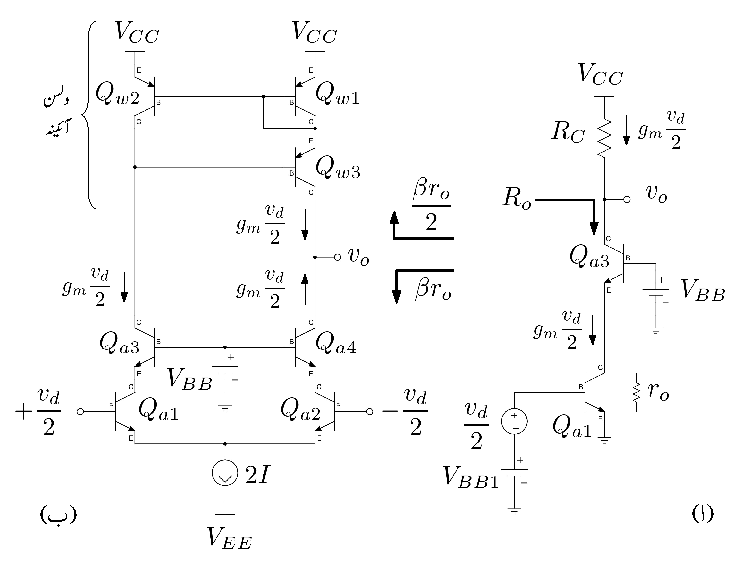
\includegraphics[scale=0.90]{cascodeDifferential}
\caption{کیسکوڈ ایمپلیفائر اور تفرقی کیسکوڈ ایمپلیفائر}
\label{شکل_تفرقی_کیسکوڈ}
\end{figure}

\عددیء{Q_{1a}} اور \عددیء{Q_{3a}} کو \عددیء{I} برقی رو پر مائل رکھا جاتا ہے۔یوں دونوں ٹرانزسٹروں کے لئے ہم لکھ سکتے ہیں۔
\begin{align*}
g_m&=\frac{I}{V_T}\\
r_e& =\frac{1}{g_m}\\
r_{be}&=\left(\beta+1 \right) r_e
\end{align*}
اگر \عددیء{Q_{1a}} کو \عددیء{\tfrac{v_d}{2}} داخلی اشارہ مہیا کیا جائے تو اس کا \عددیء{i_{c1}=g_m \tfrac{v_d}{2}} ہو گا۔یہی برقی رو \عددیء{Q_{3a}} سے بھی گزرے گا یوں \عددیء{i_{e3}=i_{c1}} ہو گا لہٰذا \عددیء{\alpha \approx 1} لیتے ہوئے\عددیء{i_{c3} =i_{c1}=g_m \tfrac{v_d}{2}} ہی ہو گا۔اس طرح \عددیء{v_o=-g_m R_C \tfrac{v_d}{2}} ہو گا۔

آئیں کیسکوڈ ایمپلیفائر کا باریک اشاراتی خارجی مزاحمت \عددیء{R_o} حاصل کریں۔باریک اشاراتی تجزیہ کرتے ہوئے ہم دیکھتے ہیں کہ \عددیء{Q_{3a}} کے ایمٹر اور برقی زمین کے مابین \عددیء{Q_{1a}} کا \عددیء{r_o} نسب ہے جبکہ \عددیء{Q_{3a}} کا بیس برقی زمین پر ہے۔ایسی صورت میں مساوات \حوالہ{مساوات_تفرقی_قابو_زمین_مخارج_مزاحمت_خارجی_مزاحمت} اور مساوات \حوالہ{مساوات_تفرقی_قابو_زمین_مخارج_مزاحمت_خارجی_مزاحمت_الف} کی مدد سے \عددیء{R_o} حاصل کیا جا سکتا ہے۔موجودہ مسئلے میں \عددیء{R_E} کی جگہ \عددیء{r_o} نسب ہے لہٰذا مساوات \حوالہ{مساوات_تفرقی_قابو_زمین_مخارج_مزاحمت_خارجی_مزاحمت_الف} کو یوں لکھا جائے گا۔
\begin{align*}
R_E'=\frac{r_{be} r_o}{r_{be}+r_o}
\end{align*}
\عددیء{r_o \gg r_{be}} کی بنا پر اس مساوات سے \عددیء{R_E' \approx r_{be}} حاصل ہوتا ہے اور یوں مساوات \حوالہ{مساوات_تفرقی_قابو_زمین_مخارج_مزاحمت_خارجی_مزاحمت} سے
\begin{gather}
\begin{aligned}\label{مساوات_تفرقی_کیسکوڈ_کی_خارجی_مزاحمت}
R_o&=r_o \left(1+g_m r_{be} \right)\\
&=r_o \left(1+\beta \right)\\
&\approx  \beta r_o
\end{aligned}
\end{gather}
حاصل ہوتا ہے۔کیسکوڈ ایمپلیفائر میں \عددیء{R_C} کی جگہ ٹرانزسٹر بوجھ بھی استعمال کیا جا سکتا ہے۔

دو کیسکوڈ ایمپلیفائر کو ملا کر تفرقی کیسکوڈ حاصل ہوتا ہے۔شکل \حوالہ{شکل_تفرقی_کیسکوڈ} ب میں ایسا ہی تفرقی ایمپلیفائر دکھایا گیا ہے جہاں ولسن آئینے کو بطور برقی بوجھ استعمال کیا گیا ہے۔اس شکل میں \عددیء{Q_{a1}}، \عددیء{Q_{a3}} ایک کیسکوڈ جبکہ  \عددیء{Q_{a2}} اور \عددیء{Q_{a4}} دوسرا کیسکوڈ ہے۔انہیں ملا کر  کیسکوڈ تفرقی جوڑی حاصل کی گئی ہے۔\عددیء{Q_{w1}}، \عددیء{Q_{w2}} اور \عددیء{Q_{w3}} ولسن آئینہ ہے جسے بطور برقی بوجھ استعمال کیا گیا ہے۔

\عددیء{\alpha =1} لیتے  ہوئے تفرقی کیسکوڈ کا باریک اشاراتی حل حاصل کرتے ہیں۔\عددیء{Q_{1a}} کو \عددیء{\tfrac{v_d}{2}} داخلی اشارہ مہیا کیا گیا ہے۔یوں اس کا خارجی برقی رو \عددیء{i_{c1}=g_m \tfrac{v_d}{2}} ہو گا۔یہی برقی رو \عددیء{Q_{a3}} سے گزرتے ہوئے ولسن آئینے کو بطور داخلی برقی رو مہیا ہوتا ہے۔یوں ولسن آئینہ \عددیء{Q_{w3}} سے  \عددیء{g_m \tfrac{v_d}{2}} بطور عکس خارج کرے گا۔کیسکوڈ کے دوسری جانب \عددیء{Q_{2a}} کو \عددیء{\tfrac{-v_d}{2}} داخلی اشارہ مہیا کیا جاتا ہے۔یوں \عددیء{i_{c2}=-g_m \tfrac{v_d}{2}} ہو گا۔یہی برقی رو \عددیء{Q_{4a}} سے بھی گزرے گا۔ولسن آئینے کی خارجی مزاحمت مساوات \حوالہ{مساوات_تفرقی_ولسن_کی_خارجی_مزاحمت} کے تحت \عددیء{\tfrac{\beta r_o}{2}} ہے جبکہ کیسکوڈ کی خارجی مزاحمت مساوات \حوالہ{مساوات_تفرقی_کیسکوڈ_کی_خارجی_مزاحمت} کے تحت \عددیء{\beta r_o} ہے۔ان دونوں متوازی جڑے خارجی مزاحمتوں کی نشاندہی شکل  \حوالہ{شکل_تفرقی_کیسکوڈ} ب میں کی گئی ہے۔ان کی مجموعی مزاحمت \عددیء{\tfrac{\beta r_o}{3}} حاصل ہوتی ہے۔یوں
\begin{align*}
v_o&=\left(g_m \frac{v_d}{2}+g_m \frac{v_d}{2} \right) \frac{\beta r_o}{3}\\
&=\frac{1}{3} g_m \beta r_o v_d
\end{align*}
حاصل ہوتا ہے۔\عددیء{g_m=\tfrac{I_C}{V_T}} اور \عددیء{r_o=\tfrac{V_A}{I_C}} لکھتے ہوئے
\begin{align}
A_d=\frac{v_o}{v_d}=\frac{1}{3} \beta \left(\frac{V_A}{V_T} \right)
\end{align}
حاصل ہوتا ہے۔صفحہ \حوالہصفحہ{مساوات_تفرقی_سادہ_ترین_کی_افزائش} پر مساوات \حوالہ{مساوات_تفرقی_سادہ_ترین_کی_افزائش} سادہ تفرقی جوڑے کی افزائش دیتا ہے۔آپ دیکھ سکتے ہیں کہ کیسکوڈ تفرقی ایمپلیفائر کی افزائش  اس سے \عددیء{\tfrac{2\beta}{3}} گنا زیادہ ہے۔

 
%==================
\حصہ{ماسفیٹ کے تفرقی جوڑے}
شکل \حوالہ{شکل_تفرقی_ماسفیٹ_بنیادی_تفرقی_جوڑا} میں دو یکساں بڑھاتے ماسفیٹ پر مبنی بنیادی تفرقی جوڑا دکھایا گیا ہے۔تفرقی جوڑے میں ماسفیٹ کو افزائندہ رکھا جاتا ہے۔\اصطلاح {ارلی برقی دباو} کو نظر انداز کرتے ہوئے اسے حل کرتے ہیں۔
\begin{figure}
\centering
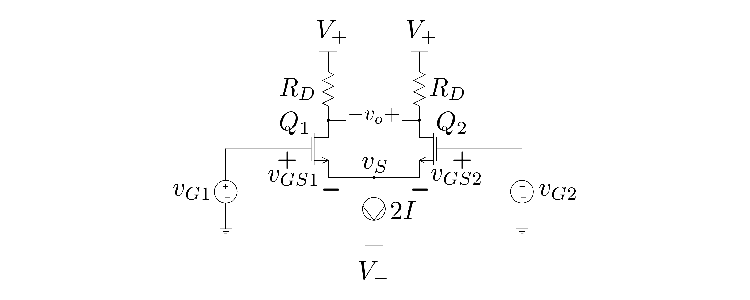
\includegraphics[scale=0.90]{mosBasicDifferencePair}
\caption{ماسفیٹ کا بنیادی تفرقی جوڑا}
\label{شکل_تفرقی_ماسفیٹ_بنیادی_تفرقی_جوڑا}
\end{figure}
تفرقی اشارہ \عددیء{v_d} سے مراد
\begin{align*}
v_d&=v_{G1}-v_{G2}
\end{align*}
ہے۔چونکہ دونوں ماسفیٹ کے سورس  آپس میں جڑے ہیں لہٰذا \عددی{v_{S1}=v_{S2}=v_S} کے برابر ہو گا۔یوں \عددی{v_{GS}=v_{G}-v_S} کو \عددی{v_{G}=v_{GS}+v_S} لکھتے ہوئے
\begin{gather}
\begin{aligned}\label{مساوات_تفرقی_اشارے_کی_دوسری_شکل}
v_d&=\left(v_{GS1}+v_S \right)-\left(v_{GS2}+v_S \right)\\
&=v_{GS1}-v_{GS2}
\end{aligned}
\end{gather}
لکھا جا سکتا ہے۔دھیان رہے کہ \عددی{v_{G1}} اور \عددی{v_{G2}} تبدیل کرنے سے \عددی{v_S} بھی تبدیل ہوتا ہے۔بدلتے اشارے کے عدم موجودگی میں \عددی{v_{GS1}=v_{GS2}=V_{GS}} ہوتا ہے۔اس صورت میں تفرقی جوڑے کے دونوں ماسفیٹ میں برابر یک سمت برقی رو گزرتی ہے۔تفرقی جوڑے میں کرخوف کے قانون برائے برقی رو کی مدد سے
\begin{align}\label{مساوات_تفرقی_دونوں_برقی_رو_کا_مجموعی_قطعی_ہے}
i_{DS1}+i_{DS2}=2I
\end{align}
لکھا جا سکتا ہے۔یوں بدلتے اشارے کے عدم موجودگی \عددی{(v_d=0)} میں اس مساوات سے \عددی{i_{DS1}=i_{DS2}=I} حاصل ہوتا ہے۔یوں ہم لکھ سکتے ہیں
\begin{align}\label{مساوات_تفرقی_یکسمتی_برابر_برقی_رو_کی_مساوات}
I_{DS1}=I_{DS2}=I=\frac{k_n}{2} \left(V_{GS}-V_t \right)^2
\end{align}
بدلتے اشارے کے موجودگی میں
\begin{align*}
i_{DS1}&=\frac{k_n}{2}\left(v_{GS1}-V_t \right)^2\\
i_{DS2}&=\frac{k_n}{2}\left(v_{GS2}-V_t \right)^2\\
\end{align*}
ہوں گے۔آئیں \عددی{i_{DS1}} اور \عددی{i_{DS2}} کے ایسے مساوات حاصل کریں جن کا آزاد متغیرہ صرف \عددی{v_d} ہو۔ایسا کرنے کی خاطر مندرجہ بالا دو مساوات کا  جزر    لیتے ہیں۔
 \begin{align*}
\sqrt{i_{DS1}}&=\sqrt{\frac{k_n}{2}}\left(v_{GS1}-V_t \right)\\
\sqrt{i_{DS2}}&=\sqrt{\frac{k_n}{2}}\left(v_{GS2}-V_t \right)\\
\end{align*}
\عددی{\sqrt{i_{DS1}}} سے \عددی{\sqrt{i_{DS2}}} کو منفی کرتے ہیں
\begin{align*}
\sqrt{i_{DS1}}-\sqrt{i_{DS2}}&=\sqrt{\frac{k_n}{2}} \left(v_{GS1}-v_{GS2} \right)\\
&=\sqrt{\frac{k_n}{2}} v_d
\end{align*}
جہاں مساوات \حوالہ{مساوات_تفرقی_اشارے_کی_دوسری_شکل} کو استعمال کیا گیا۔مساوات \حوالہ{مساوات_تفرقی_دونوں_برقی_رو_کا_مجموعی_قطعی_ہے} سے \عددی{i_{DS2}} حاصل کر کے مندرجہ بالا مساوات میں پُر کرتے ہیں۔
\begin{align*}
\sqrt{i_{DS1}}-\sqrt{2I -i_{DS1}}&=\sqrt{\frac{k_n}{2}} v_d
\end{align*}
اس مساوات کا مربع لیتے ہیں
\begin{align*}
i_{DS1}+2I -i_{DS1} -2\sqrt{i_{DS1}} \sqrt{2I-i_{DS1}} =\frac{k_n}{2} v_d^2\\
2\sqrt{i_{DS1}} \sqrt{2I-i_{DS1}}=2I-\frac{k_n}{2} v_d^2
\end{align*}
اس کا دوبارہ مربع لیتے  ہوئے دو درجی مساوات حاصل ہوتی ہے
\begin{align*}
4 i_{DS1} \left(2I-i_{DS1} \right)=4I^2+\frac{k_n^2}{4} v_d^4-2I k_n v_d^2\\
4 i_{DS1}^2-8 I i_{DS1}+4 I^2+\frac{k_n^2}{4} v_d^4-2 I k_n v_d^2=0
\end{align*}
جس سے
\begin{align*}
i_{DS1}&=\frac{8 I \mp\sqrt{64 I^2 -4 \times 4 \times \left(4 I^2+\frac{k_n^2}{4} v_d^4-2 I k_n v_d^2 \right)}}{2 \times 4}\\
&=I \mp \frac{\sqrt{2 I k_n v_d^2 -\frac{k_n^2}{4} v_d^4}}{2}\\
&=I \mp \left(\frac{v_d}{2} \right)\sqrt{2 I k_n} \sqrt{1-\frac{k_n}{2 I} \left(\frac{v_d}{2} \right)^2}
\end{align*}
حاصل ہوتا ہے۔بدلتے اشارے کے عدم موجودگی \عددی{(v_d=0)} کی صورت میں اس مساوات سے \عددی{i_{DS1}=I} حاصل ہوتا ہے جو کہ درست جواب ہے۔شکل \حوالہ{شکل_تفرقی_ماسفیٹ_بنیادی_تفرقی_جوڑا} کو دیکھ کر ہم کہہ سکتے ہیں کہ  مثبت \عددی{v_d} کی صورت میں \عددی{i_{DS1}} کی قیمت \عددی{I} سے بڑھ جائے گی۔یوں مندرجہ بالا مساوات سے \عددی{i_{DS1}} کا درست مساوات یوں لکھا جائے گا۔
\begin{align}\label{مساوات_تفرقی_پہلے_ماسفیٹ_کا_برقی_رو}
i_{DS1}=I + \left(\frac{v_d}{2} \right)\sqrt{2 I k_n} \sqrt{1-\frac{k_n}{2 I} \left(\frac{v_d}{2} \right)^2}
\end{align}
مساوات \حوالہ{مساوات_تفرقی_دونوں_برقی_رو_کا_مجموعی_قطعی_ہے} کی مدد سے 
\begin{align*}
i_{DS2}&=2I-i_{DS1}\\
&=2I-\left[I + \left(\frac{v_d}{2} \right)\sqrt{2 I k_n} \sqrt{1-\frac{k_n}{2 I} \left(\frac{v_d}{2} \right)^2} \right]
\end{align*}
یعنی
\begin{align}\label{مساوات_تفرقی_دوسرے_ماسفیٹ_کا_برقی_رو}
i_{DS2}=I - \left(\frac{v_d}{2} \right)\sqrt{2 I k_n} \sqrt{1-\frac{k_n}{2 I} \left(\frac{v_d}{2} \right)^2}
\end{align}
حاصل ہوتا ہے۔

مساوات \حوالہ{مساوات_تفرقی_یکسمتی_برابر_برقی_رو_کی_مساوات} کو ان دو طرز
\begin{align*}
\sqrt{k_n}&=\frac{\sqrt{2I}}{V_{GS}-V_t}\\
\frac{k_n}{2I}&=\frac{1}{\left(V_{GS}-V_t \right)^2}
\end{align*}
پر بھی لکھا جا سکتا ہے جن کے استعمال سے  مساوات \حوالہ{مساوات_تفرقی_پہلے_ماسفیٹ_کا_برقی_رو} اور مساوات \حوالہ{مساوات_تفرقی_دوسرے_ماسفیٹ_کا_برقی_رو}
کو یوں لکھا جا سکتا ہے۔
\begin{gather}
\begin{aligned}\label{مساوات_تفرقی_دونوں_ماسفیٹ_کا_برقی_رو}
i_{DS1}&=I+\left(\frac{v_d}{2}\right) \frac{2I}{V_{GS}-V_t} \sqrt{1-\frac{1}{\left(V_{GS}-V_t \right)^2} \left(\frac{v_d}{2} \right)^2}\\
i_{DS2}&=I-\left(\frac{v_d}{2}\right) \frac{2I}{V_{GS}-V_t} \sqrt{1-\frac{1}{\left(V_{GS}-V_t \right)^2} \left(\frac{v_d}{2} \right)^2}
\end{aligned}
\end{gather}
صفحہ \حوالہصفحہ{مساوات_میدانی_باریک_اشارہ_کی_شرط} پر مساوات \حوالہ{مساوات_میدانی_باریک_اشارہ_کی_شرط} باریک اشارے کی تعریف
  \عددی{v_d \ll 2 \left(V_{GS}-V_t \right)} دیتا ہے۔اگر داخلی اشارہ اس شرط پر پورا اترتا ہو تب  مساوات \حوالہ{مساوات_تفرقی_دونوں_ماسفیٹ_کا_برقی_رو} میں  جزر    کے اندر ایک سے منفی ہونے والے حصے کو نظر انداز کیا جا سکتا ہے اور ان مساوات کو یوں لکھا جا سکتا ہے۔
\begin{gather}
\begin{aligned}\label{مساوات_تفرقی_دونوں_ماسفیٹ_کا_برقی_رو_خطی_مساوات}
i_{DS1}& \approx I+\left(\frac{v_d}{2}\right) \frac{2I}{V_{GS}-V_t} \\
i_{DS2}& \approx I-\left(\frac{v_d}{2}\right) \frac{2I}{V_{GS}-V_t}
\end{aligned}
\end{gather}
صفحہ \حوالہصفحہ{مساوات_ماسفیٹ_باریک_افزائش_کے_مختلف_مساوات} پر مساوات \حوالہ{مساوات_ماسفیٹ_باریک_افزائش_کے_مختلف_مساوات} کے تحت
\begin{align*}
g_m=\frac{2 I_{DS}}{V_{GS}-V_t}
\end{align*}
کے برابر ہے جہاں \عددی{I_{DS}} ماسفیٹ سے گزرتی یک سمت برقی رو ہے۔مساوات \حوالہ{مساوات_تفرقی_دونوں_ماسفیٹ_کا_برقی_رو_خطی_مساوات} میں یک سمت برقی رو کو \عددی{I} کہا گیا ہے۔یوں مساوات \حوالہ{مساوات_تفرقی_دونوں_ماسفیٹ_کا_برقی_رو_خطی_مساوات} کو
\begin{gather}
\begin{aligned}\label{مساوات_تفرقی_دونوں_ماسفیٹ_کا_برقی_رو_خطی_مساوات_الف}
i_{DS1}& \approx I+g_m \left(\frac{v_d}{2}\right) \\
i_{DS2}& \approx I-g_m \left(\frac{v_d}{2}\right)
\end{aligned}
\end{gather}
لکھا جا سکتا ہے۔مساوات \حوالہ{مساوات_تفرقی_دونوں_ماسفیٹ_کا_برقی_رو_خطی_مساوات_الف} کا انتہائی سادہ مطلب ہے۔مثبت بدلتے برقی اشارے کے موجودگی میں \عددی{i_{DS1}} کی قیمت  میں \عددی{g_m \tfrac{v_d}{2}}  کا اضافہ ہوتا ہے جبکہ \عددی{i_{DS2}} کی قیمت میں اتنی ہی کمی رونما ہوتی ہے۔\عددی{i_{DS1}} جمع \عددی{i_{DS2}} اب بھی \عددی{2I} کے برابر ہے۔\عددی{i_{DS1}} اور \عددی{i_{DS2}} میں اس بدلتا برقی رو کو \عددی{i_d} لکھا جا سکتا ہے یعنی
\begin{align}
i_d=g_m \left(\frac{v_d}{2} \right)
\end{align} 
یوں
\begin{gather}
\begin{aligned}
i_{DS1}&=I+i_d\\
i_{DS2}&=I-i_d
\end{aligned}
\end{gather}
کے برابر ہیں۔\عددی{v_d} کی وہ قیمت جس پر تمام کی تمام \عددی{2I} یک سمت برقی رو کسی ایک ماسفیٹ میں منتقل ہو جاتی ہے کو مساوات \حوالہ{مساوات_تفرقی_دونوں_ماسفیٹ_کا_برقی_رو} کی مدد سے حاصل کیا جا سکتا ہے۔مثبت \عددی{v_d} کی صورت میں برقی رو \عددی{Q_1} کو منتقل ہو گی۔یوں \عددی{i_{DS1}=2I} جبکہ \عددی{i_{DS2}=0} ہوں گے۔مساوات \حوالہ{مساوات_تفرقی_دونوں_ماسفیٹ_کا_برقی_رو} میں \عددی{i_{DS1}=2ِ}  پُر کرتے حل کرنے سے
\begin{align}\label{مساوات_تفرقی_جوڑے_کو_درکار_زیادہ_سے_زیادہ_داخلی_برقی_دباو}
\abs{v_{d}}_{بلندتر}= \sqrt{2} \left(V_{GS}-V_t \right)
\end{align} 
حاصل ہوتا ہے۔اس قیمت سے \عددی{v_d} کو مزید بڑھانے سے برقی رو میں مزید تبدیلی رونما نہیں ہو گی۔اتنی ہی منفی داخلی برقی دباو کی صورت میں تمام کی تمام یک سمت برقی رو \عددی{Q_2} کو منتقل ہو جائے گی اور یوں \عددی{i_{DS1}=0} جبکہ \عددی{i_{DS2}=2I} ہوں گے۔شکل \حوالہ{شکل_تفرقی_داخلی_برقی_دباو_بالمقابل_برقی_رو} میں مساوات \حوالہ{مساوات_تفرقی_دونوں_ماسفیٹ_کا_برقی_رو} کے خط کھینچے گئے ہیں۔ان خطوط سے آپ دیکھ سکتے ہیں کہ \عددیء{v_d} کی وہ قیمت جس پر تمام کی تمام برقی رو ایک جانب منتقل ہو جاتی ہے  صفحہ \حوالہصفحہ{مساوات_میدانی_باریک_اشارہ_کی_شرط} پر مساوات \حوالہ{مساوات_میدانی_باریک_اشارہ_کی_شرط} میں بیان کئے باریک اشارے کی حد سے کم ہے۔
\begin{figure}
\centering
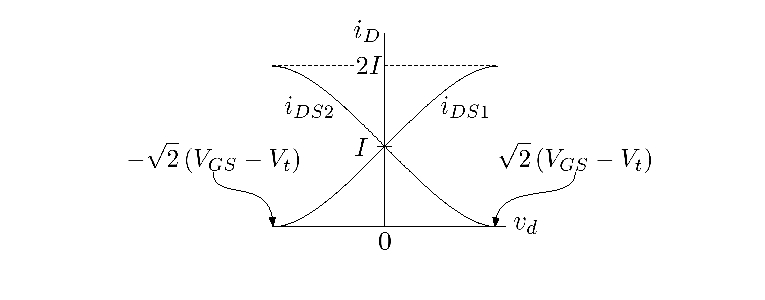
\includegraphics[scale=0.90]{differencePairInputVoltageVersusOutputCurrentCurveOctave}
\caption{ماسفیٹ تفرقی جوڑے کے داخلی تفرقی برقی دباو بالمقابل خارجی برقی رو کے خط}
\label{شکل_تفرقی_داخلی_برقی_دباو_بالمقابل_برقی_رو}
\end{figure}

شکل \حوالہ{شکل_تفرقی_ماسفیٹ_بنیادی_تفرقی_جوڑا} سے 
\begin{align*}
v_{D1}&=V_{+} - i_{DS1} R_D\\
v_{D2}&=V_{+}-i_{DS2} R_D
\end{align*}
اور
\begin{align*}
v_0&=v_{D2}-v_{D1}\\
&=(V_{+}-i_{DS2} R_D)-(V_{+} - i_{DS1} R_D)\\
&=i_{DS1}R_D-i_{DS2} R_D
\end{align*}
لکھتے ہوئے  مساوات \حوالہ{مساوات_تفرقی_دونوں_ماسفیٹ_کا_برقی_رو_خطی_مساوات_الف} کے استعمال سے
\begin{align*}
v_o&=\left[I+g_m \frac{v_d}{2}\right]R_D-\left[I-g_m \frac{v_d}{2} \right] R_D\\
&=g_m v_d R_D
\end{align*}
ملتا ہے جس سے تفرقی افزائش
\begin{align}\label{مساوات_تفرقی_بنیادی_جوڑے_کی_افزائش}
A_d=\frac{v_o}{v_d}=g_m R_D
\end{align}
حاصل ہوتی ہے۔
%=============================
\ابتدا{مثال}\شناخت{مثال_تفرقی_درکار_زیادہ_سے_زیادہ_داخلی_برقی_دباو}
شکل \حوالہ{شکل_تفرقی_ماسفیٹ_بنیادی_تفرقی_جوڑا} میں دکھائے گئے ماسفیٹ کے تفرقی جوڑے میں \عددی{2I=\SI{200}{\micro \ampere}} ہے جبکہ \عددی{k_n=\SI[per=frac,fraction=nice]{0.1}{\milli \ampere \per \volt \squared}} اور \عددی{V_t=\SI{1.2}{\volt}} ہیں۔\عددیء{V_{GS}} اور \عددیء{g_m} حاصل کرتے ہوئے \عددی{v_d} کی وہ قیمت حاصل کریں جس پر تمام کی تمام برقی رو ایک ماسفیٹ کو منتقل ہو جاتی ہے۔

حل:\عددی{v_d=0} پر دونوں ماسفیٹ اپنے نقطہ کارکردگی پر ہوتے ہیں اور دونوں میں برابر \عددی{\SI{100}{\micro \ampere}} برقی رو پایا جاتا ہے۔افزائندہ ماسفیٹ کی مساوات سے یوں
\begin{align*}
100 \times 10^{-6}&=\frac{0.1 \times 10^{-3}}{2} \left(V_{GS}-1.2 \right)^2
\end{align*}
لکھتے ہوئے \عددی{\SI{2.614}{\volt}} حاصل ہوتا ہے۔صفحہ \حوالہصفحہ{مساوات_ماسفیٹ_باریک_افزائش_کے_مختلف_مساوات} پر مساوات \حوالہ{مساوات_ماسفیٹ_باریک_افزائش_کے_مختلف_مساوات} کے استعمال سے
\begin{align*}
g_m=\sqrt{2 \times 100 \times 10^{-6} \times 0.1 \times 10^{-3}}=\SI{0.1414}{\milli \siemens}
\end{align*}
اور مساوات \حوالہ{مساوات_تفرقی_جوڑے_کو_درکار_زیادہ_سے_زیادہ_داخلی_برقی_دباو} سے
\begin{align*}
\abs{v_d}=\sqrt{2} \left(2.614-1.2 \right)=\SI{2}{\volt}
\end{align*}
حاصل ہوتا ہے۔یوں \عددی{v_d=\SI{2}{\volt}} پر تمام برقی رو \عددی{Q_1} سے  گزرے گا جبکہ \عددی{v_d=\SI{-2}{\volt}} پر تمام برقی رو \عددی{Q_2} سے گزرے گا۔
\انتہا{مثال}
%==================
\ابتدا{مثال}
مثال \حوالہ{مثال_تفرقی_درکار_زیادہ_سے_زیادہ_داخلی_برقی_دباو} میں \عددی{V_{+}=\SI{18}{\volt}} جبکہ \عددی{R_D=\SI{50}{\kilo \ohm}} کی صورت میں تفرقی جوڑے  کی تفرقی افزائش حاصل کریں۔

حل:مساوات \حوالہ{مساوات_تفرقی_بنیادی_جوڑے_کی_افزائش} کی مدد سے
\begin{align*}
A_d=0.1414 \times 10^{-3} \times 50000=\SI{7.07}{\volt \per \volt}
\end{align*} 
حاصل ہوتا ہے۔
\انتہا{مثال}
%===========
\ابتدا{مثال}\شناخت{مثال_تفرقی_مخارج_برقی_دباو_کا_حصول}
شکل \حوالہ{شکل_تفرقی_ماسفیٹ_بنیادی_تفرقی_جوڑا} میں دکھائے گئے ماسفیٹ کے تفرقی جوڑے میں \عددی{2I=\SI{200}{\micro \ampere}} ہے جبکہ \عددی{k_n=\SI[per=frac,fraction=nice]{0.1}{\milli \ampere \per \volt \squared}} اور \عددی{V_t=\SI{1.2}{\volt}} ہیں۔\عددی{Q_2} کو برقی زمین پر رکھتے ہوئے  \عددیء{v_{GS1}}، \عددیء{v_{GS2}}، \عددیء{v_{S}} اور \عددی{v_{G1}} کی قیمتیں مندرجہ ذیل صورتوں میں حاصل کریں۔
\begin{enumerate}
\item
\عددی{i_{DS1}=\SI{100}{\micro \ampere}} ہے۔
\item
\عددی{i_{DS1}=\SI{150}{\micro \ampere}} ہے۔
\item
\عددی{i_{DS1}=\SI{200}{\micro \ampere}} ہے۔
\end{enumerate} 

حل:
\begin{enumerate}
\item
\عددی{i_{DS1}=\SI{100}{\micro \ampere}} کی صورت میں مساوات \حوالہ{مساوات_تفرقی_دونوں_برقی_رو_کا_مجموعی_قطعی_ہے} کے تحت \عددی{i_{DS2}=\SI{100}{\micro \ampere}} ہو گی۔اس صورت میں دونوں ماسفیٹ میں برابر برقی رو ہو گا۔افزائندہ ماسفیٹ کی مساوات سے
\begin{align*}
100 \times 10^{-6}=\frac{0.1 \times 10^{-3}}{2}\left(v_{GS1}-1.2 \right)^2
\end{align*}
سے \عددی{v_{GS1}=\SI{2.614}{\volt}} حاصل ہوتے ہیں۔\عددی{v_{GS2}} بھی اتنا ہی ہو گا۔

یہاں غور کریں۔ہمیں \عددی{v_{GS1}} معلوم ہے لیکن ہمیں \عددی{v_{G1}} معلوم نہیں ہے۔اس کے برعکس ہمیں \عددی{v_{GS2}} معلوم ہونے کے ساتھ ساتھ یہ بھی معلوم ہے کہ اس \عددی{Q_2} کے گیٹ برقی زمین پر ہے۔یوں ہم جانتے ہیں کہ \عددی{v_{G2}=\SI{0}{\volt}} پر ہے۔

\عددی{v_{GS2}=v_{G2}-v_S} لکھتے ہوئے اور \عددی{v_S=\SI{-2.614}{\volt}} حاصل
 ہوتا ہے۔\عددی{v_{GS1}=v_{G1}-v_S} میں حاصل کردہ \عددی{v_S} اور \عددی{v_{GS1}} کی قیمتیں پُر کرنے سے \عددی{v_{G1}=\SI{0}{\volt}} حاصل ہوتا ہے۔
\item
\عددی{i_{DS1}=\SI{150}{\micro \ampere}} کی صورت میں مساوات \حوالہ{مساوات_تفرقی_دونوں_برقی_رو_کا_مجموعی_قطعی_ہے} کے تحت \عددی{i_{DS2}=\SI{50}{\micro \ampere}} ہو گی۔افزائندہ ماسفیٹ کے مساوات سے دونوں ماسفیٹ کے \عددی{v_{GS}} حاصل کرتے ہیں۔\عددی{Q_1} کے مساوات سے
\begin{align*}
150 \times 10^{-6}&=\frac{0.1 \times 10^{-3}}{2}\left(v_{GS1}-1.2 \right)^2\\
v_{GS1}&=\SI{2.932}{\volt}
\end{align*}
اور \عددی{Q_2} کے مساوات سے
\begin{align*}
50 \times 10^{-6}&=\frac{0.1 \times 10^{-3}}{2}\left(v_{GS2}-1.2 \right)^2\\
v_{GS2}&=\SI{2.2}{\volt}
\end{align*}
حاصل ہوتے ہیں۔\عددی{Q_2} کے معلومات سے
\begin{align*}
v_{GS2}=v_{G2}-v_S=0-v_S
\end{align*}
سے \عددی{v_S=\SI{-2.2}{\volt}} اور یوں 
\begin{align*}
v_{GS1}&=v_{G1}-v_S\\
2.932&=v_{G1}-\left(-2.2 \right)\\
v_{G1}&=\SI{0.732}{\volt}
\end{align*}
حاصل ہوتا ہے۔
\item
\عددی{i_{DS1}=\SI{200}{\micro \ampere}} کی صورت میں مساوات \حوالہ{مساوات_تفرقی_دونوں_برقی_رو_کا_مجموعی_قطعی_ہے} کے تحت \عددی{i_{DS2}=\SI{0}{\micro \ampere}} ہو گی۔\عددی{Q_1} کے مساوات سے
\begin{align*}
200 \times 10^{-6}&=\frac{0.1 \times 10^{-3}}{2} \left(v_{GS1}-1.2 \right)^2\\
v_{GS1}&=\SI{3.2}{\volt}
\end{align*}
اور \عددی{Q_2} کے مساوات سے
\begin{align*}
0&=\frac{0.1 \times 10^{-3}}{2} \left(v_{GS2}-1.2 \right)^2\\
v_{GS2}&=\SI{1.2}{\volt}
\end{align*}
حاصل ہوتے ہیں۔یوں
\begin{align*}
v_{GS2}&=v_{G2}-v_S\\
1.2&=0-v_S
\end{align*}
سے \عددی{v_S=\SI{-1.2}{\volt}} اور 
\begin{align*}
v_{GS1}&=v_{G1}-v_S\\
3.2&=v_{G1}-\left(-1.2 \right)\\
v_{G1}&=\SI{2}{\volt}
\end{align*}
حاصل ہوتے ہیں۔
\end{enumerate}
\انتہا{مثال}
%========================
\ابتدا{مثال}
مثال \حوالہ{مثال_تفرقی_مخارج_برقی_دباو_کا_حصول} میں \عددی{v_{G1}=\SI{4}{\volt}} کی صورت میں \عددیء{v_{GS1}}، \عددیء{v_{GS2}}، \عددیء{v_{S}} اور \عددی{v_{G1}} کی قیمتیں  حاصل کریں۔

حل:مثال \حوالہ{مثال_تفرقی_مخارج_برقی_دباو_کا_حصول} میں دیکھا گیا کہ \عددی{v_{GS1}=\SI{3.2}{\volt}} کرنے سے تمام کی تمام برقی رو \عددی{Q_1} کو منتقل ہو جاتی ہے۔\عددی{Q_1} کے گیٹ پر برقی دباو مزید بڑھانے سے \عددی{i_{DS1}} پر کوئی اثر نہیں پڑتا اور یہ \عددی{\SI{200}{\micro \ampere}} ہی رہتی ہے۔یوں \عددی{v_{GS1}=\SI{3.2}{\volt}} ہی رہے گا۔یوں
\begin{align*}
v_{GS1}&=v_{G1}-v_S\\
3.2&=4-v_S
\end{align*}
سے \عددی{v_S=\SI{0.8}{\volt}} حاصل ہوتا ہے اور یوں
\begin{align*}
v_{GS2}&=v_{G2}-v_S\\
&=0-0.8\\
&=\SI{-0.8}{\volt}
\end{align*}
ہو گا۔اس صورت میں چونکہ \عددی{v_{GS2} < V_t} ہے لہٰذا \عددی{Q_2} منقطع ہو گا۔
\انتہا{مثال}

%=====================
\حصہ{داخلی انحرافی برقی دباو}
ماسفیٹ کے تفرقی جوڑے میں بھی ناقص پن پایا جاتا ہے۔شکل \حوالہ{شکل_تفرقی_ماسفیٹ_بنیادی_تفرقی_جوڑا} میں \اصطلاح {داخلی انحرافی برقی دباو}\فرہنگ{داخلی!انحرافی برقی دباو}\حاشیہب{input offset voltage} تین وجوہات سے پیدا ہو سکتا ہے۔ ڈرین پر نسب مزاحمتوں میں فرق، دونوں ماسفیٹ کے \عددی{\tfrac{W}{L}} میں فرق اور دونوں ماسفیٹ کے \عددی{V_t} میں فرق وہ تین وجوہات ہیں۔آئیں ان کے اثر کو باری باری دیکھیں۔
\begin{gather}
\begin{aligned}
R_{D1}&=R_D+\Delta R_D\\
R_{D2}&=R_D-\Delta R_D
\end{aligned}
\end{gather}
کی صورت میں دونوں ماسفیٹ میں برابر برقی رو \عددی{I} تصور کرتے ہوئے
\begin{align*}
V_{D1}&=V_{+}-I \left(R_D+\Delta R_D \right)\\
V_{D2}&=V_{+}-I \left(R_D-\Delta R_D \right)\\
V_O&=V_{DS2}-V_{DS1}=2 I\Delta R_D 
\end{align*}
حاصل ہوتا ہے جس کو \عددی{A_d} سے تقسیم کرنے سے داخلی انحرافی برقی دباو حاصل ہوتا ہے۔\عددی{A_d} کو مساوات \حوالہ{مساوات_تفرقی_بنیادی_جوڑے_کی_افزائش} پیش کرتا ہے۔صفحہ \حوالہصفحہ{مساوات_ماسفیٹ_باریک_افزائش_کے_مختلف_مساوات} پر مساوات \حوالہ{مساوات_ماسفیٹ_باریک_افزائش_کے_مختلف_مساوات} کے تحت \عددی{g_m=\tfrac{2 I_{DS}}{V_{GS}-V_t}} کے برابر ہے۔یہاں \عددی{I_{DS}}  کو \عددی{I} کہا گیا ہے۔یوں
\begin{align*}
A_d=g_m R_D=\left(\frac{2 I}{V_{GS}-V_t}\right) R_D
\end{align*} 
لکھتے ہوئے
\begin{align*}
V_{OS}&=\frac{V_O}{A_d}\\
&=\frac{2 I\Delta R_D }{\left(\frac{2 I}{V_{GS}-V_t}\right) R_D}
\end{align*}
یعنی
\begin{align}
V_{OS}=\left(V_{GS}-V_t \right)\left(\frac{\Delta R}{R}\right)
\end{align}
حاصل ہوتا ہے۔

آئیں اب \عددی{k_n} میں فرق کے اثرات کو دیکھیں۔تصور کریں کہ
\begin{gather}
\begin{aligned}
\left(\frac{W}{L}\right)_1&=\frac{W}{L}+\Delta \left(\frac{W}{L}\right)\\
\left(\frac{W}{L}\right)_2&=\frac{W}{L}-\Delta \left(\frac{W}{L}\right)
\end{aligned}
\end{gather}
ہیں۔ایسی صورت میں
\begin{align*}
i_{DS1}&=\frac{k_{n1}}{2} \left(V_{GS}-V_t\right)^2\\
i_{DS2}&=\frac{k_{n2}}{2} \left(V_{GS}-V_t\right)^2
\end{align*}
ہوں گے۔\عددی{i_{DS2}} کے مساوات کو \عددی{i_{DS1}} کی مساوات سے تقسیم کرتے ہوئے
\begin{align*}
\frac{i_{DS2}}{i_{DS1}}=\frac{\frac{k_{n2}}{2} \left(V_{GS}-V_t\right)^2}{\frac{k_{n1}}{2} \left(V_{GS}-V_t\right)^2}=\frac{k_{n2}}{k_{n1}}
\end{align*}
ملتا ہے جس کے دونوں جانب ایک جمع کرتے  ہوئے
\begin{align*}
\frac{i_{DS2}}{i_{DS1}}+1&=\frac{k_{n2}}{k_{n1}}+1\\
\frac{i_{DS2}+i_{DS1}}{i_{DS1}}&=\frac{k_{n2}+k_{n1}}{k_{n1}}\\
\frac{2 I}{i_{DS1}}&=\frac{k_{n2}+k_{n1}}{k_{n1}}
\end{align*}
حاصل ہوتا ہے جہاں تیسرے قدم پر مساوات \حوالہ{مساوات_تفرقی_دونوں_برقی_رو_کا_مجموعی_قطعی_ہے} کے تحت \عددی{i_{DS1}+i_{DS2}=2I} لکھا گیا۔مندرجہ بالا مساوات کو الٹا کرتے ہوئے
\begin{align*}
\frac{i_{DS1}}{2I}&=\frac{k_{n1}}{k_{n2}+k_{n1}}\\
&=\frac{k_n' \left[\frac{W}{L}+\Delta \left(\frac{W}{L}\right) \right]}{k_n' \left[\frac{W}{L}-\Delta \left(\frac{W}{L}\right)+\frac{W}{L}+\Delta \left(\frac{W}{L}\right) \right]}\\
&=\frac{\left[\frac{W}{L}+\Delta \left(\frac{W}{L}\right) \right]}{2 \frac{W}{L}}
\end{align*}
لکھا جا سکتا ہے جس سے
\begin{align}
i_{DS1}=I \left[1+\frac{\Delta \left(\frac{W}{L} \right)}{\frac{W}{L}}\right]
\end{align}
حاصل ہوتا ہے۔مساوت \حوالہ{مساوات_تفرقی_دونوں_برقی_رو_کا_مجموعی_قطعی_ہے} کو استعمال کرتے ہوئے
\begin{align*}
i_{DS2}&=2 I -i_{DS1}\\
&=2 I-I \left[1+\frac{\Delta \left(\frac{W}{L} \right)}{\frac{W}{L}}\right]
\end{align*}
سے
\begin{align}\label{مساوات_تفرقی_رقبے_میں_فرق_سے_دوسری_برقی_رو}
i_{DS2}=I \left[1-\frac{\Delta \left(\frac{W}{L} \right)}{\frac{W}{L}}\right]
\end{align}
حاصل ہوتا ہے۔ان \عددی{i_{DS1}} اور \عددی{i_{DS2}} کے استعمال سے
\begin{align}\label{مساوات_تفرقی_رقبے_میں_فرق_سے_داخلی_انحرافی_برقی_دباو}
V_{OS}=\left(V_{GS}-V_t \right)\left[\frac{\Delta \left(\frac{W}{L}\right)}{\frac{W}{L}}\right]
\end{align}
حاصل ہوتا ہے۔

آخر میں دونوں ماسفیٹ کے \عددی{V_t} میں فرق کے اثرات کو دیکھتے ہیں۔فرض کریں کہ
\begin{gather}
\begin{aligned}
V_{t1}&=V_t+\Delta V_t\\
V_{t2}&=V_t-\Delta V_t
\end{aligned}
\end{gather}
ہیں۔اس صورت میں

\begin{align*}
i_{DS1}&=\frac{k_n}{2} \left(V_{GS}-V_t-\Delta V_t \right)^2\\
&=\frac{k_n}{2} \left(V_{GS}-V_t \right)^2 \left(1-\frac{\Delta V_t}{V_{GS}-V_t} \right)^2\\
i_{DS2}&=\frac{k_n}{2} \left(V_{GS}-V_t+\Delta V_t \right)^2\\
&=\frac{k_n}{2} \left(V_{GS}-V_t \right)^2 \left(1+\frac{\Delta V_t}{V_{GS}-V_t} \right)^2
\end{align*}
لکھا جا سکتا ہے جہاں \عددی{\left(V_{GS}-V_t \right)} کو قوصین کے باہر لایا گیا۔دونوں مساوات میں دائیں جانب قوصین کھولتے ہیں۔
\begin{align*}
i_{DS1}&=\frac{k_n}{2} \left(V_{GS}-V_t \right)^2 \left[1-\frac{2 \Delta V_t}{V_{GS}-V_t}+\left(\frac{\Delta V_t}{V_{GS}-V_t}\right)^2   \right]\\
i_{DS2}&=\frac{k_n}{2} \left(V_{GS}-V_t \right)^2 \left[1+\frac{2 \Delta V_t}{V_{GS}-V_t}+\left(\frac{\Delta V_t}{V_{GS}-V_t}\right)^2   \right]
\end{align*}
اگر  \عددی{\Delta V_t \ll \left(V_{GS}-V_t \right)} ہو تب \عددی{\left(\frac{\Delta V_t}{V_{GS}-V_t} \right)^2}  کو نظر انداز کیا جا سکتا ہے۔یوں
\begin{align*}
i_{DS1}&=\frac{k_n}{2} \left(V_{GS}-V_t \right)^2 \left[1-\frac{2 \Delta V_t}{V_{GS}-V_t}\right]\\
i_{DS2}&=\frac{k_n}{2} \left(V_{GS}-V_t \right)^2 \left[1+\frac{2 \Delta V_t}{V_{GS}-V_t}\right]
\end{align*}
حاصل ہوتے ہیں۔ان مساوات میں
\begin{align*}
I=\frac{k_n}{2} \left(V_{GS}-V_t \right)^2 
\end{align*}
پُر کرنے سے انہیں
\begin{align*}
i_{DS1}&=I \left[1-\frac{2 \Delta V_t}{V_{GS}-V_t}\right]\\
i_{DS2}&=I \left[1+\frac{2 \Delta V_t}{V_{GS}-V_t}\right]
\end{align*}
لکھا جا سکتا ہے۔یوں
\begin{align*}
v_{D1}&=V_{+}- i_{DS1} R_D\\
v_{D2}&=V_{+}-i_{DS2} R_D
\end{align*}
سے
\begin{align*}
V_O&=\left(i_{DS1}-i_{DS2} \right) R_D\\
&=-4 I R_D\left(\frac{\Delta V_t}{V_{GS}-V_t}\right)
\end{align*}
اور
\begin{align}
V_{OS}&=\frac{V_O}{A_d}=- 2 \Delta V_t
\end{align}
حاصل ہوتا ہے۔
\عددیء{\Delta R_S} اور \عددی{\Delta \left(\tfrac{W}{L} \right)} کی وجہ سے پیدا \عددیء{V_{OS}} کو کم رکھنے کی خاطر ماسفیٹ کو کم سے کم \عددیء{\left(V_{GS}-V_t \right)} پر چلایا جاتا ہے۔دو جوڑ ٹرانزسٹر کے تفرقی جوڑے میں داخلی انحرافی برقی دباو دونوں بازووں  کے \عددی{R_C} میں فرق اور دونوں ٹرانزسٹروں کے \عددی{I_S} میں فرق کی بنا پر پیدا ہوتا ہے۔ماسفیٹ کے تفرقی جوڑے میں داخلی انحرافی برقی دباو پیدا کرنے کی تیسری وجہ \عددی{V_t} بھی پائی جاتی ہے۔
%===================
\حصہ{ماسفیٹ آئینہ برقی رو}
شکل \حوالہ{شکل_تفرقی_سادہ_آئینے_کی_خارجی_مزاحمت} میں ماسفیٹ کا سادہ آئینہ برقی رو دکھایا گیا ہے جس کو دیکھتے ہی ہم کہہ سکتے ہیں کہ \عددیء{R_o=r_{o}} کے برابر ہے۔آئیں یہی نتیجہ ماسفیٹ ریاضی نمونہ استعمال کرتے ہوئے حاصل کریں۔خارجی مزاحمت حاصل کرنے کی خاطر \عددیء{Q_2} کے ڈرین پر باریک اشاراتی \عددیء{v_t} لاگو کرتے ہوئے \عددیء{i_t} کا تخمینہ لگا کر \عددیء{\tfrac{v_t}{i_t}} سے خارجی مزاحمت \عددیء{R_o} حاصل کیا جا سکتا ہے۔
\begin{figure}
\centering
\begin{subfigure}{0.4\textwidth}
\centering
\begin{tikzpicture}
\draw (0,0) node[nmos,anchor=source,xscale=-1](Q1){}
      ++(\x,0) node[nmos,anchor=source,xscale=1](Q2){};
\draw(Q1.gate)--(Q2.gate);
\draw(Q1.gate)node[below]{$V_G$}node[circ]{}|-(Q1.drain)node[circ]{};
\draw (Q1.source)node[right]{$Q1$} (Q2.source)node[left]{$Q2$};
\draw(Q1.source)to [short,-o]++(0,-0.5){}node[below]{$V_{EE}$};
\draw(Q2.source) to [short,-o]++(0,-0.5){}node[below]{$V_{EE}$};
\draw(Q1.drain) to [american current source,invert]++(0,\y) to [short,-o]++(0,0.25)node[right]{$V_{DD}$};
\draw(Q2.drain) to [short,-o]++(1,0);
\draw(Q2.drain)++(0.5,-0.25) to [R,/tikz/circuitikz/bipoles/length=20pt,l={$r_0$}]++(0,-1);
\draw[latex-,thick](Q2.drain)++(0.25,-0.5)--++(0,0.35)--++(1,0)node[right]{$R_0$};
\draw[dashed](Q2.drain) --++(0,1);
\end{tikzpicture}
\caption{}
\end{subfigure}\hfill
\begin{subfigure}{0.55\textwidth}
\centering
\begin{tikzpicture}
\draw(0,0)node[ground]{} to[american controlled current source,invert,l_={$g_mv_{gs}$}]++(0,\y)to [short]++(\x,0)coordinate(kR) to [R,l={$r_0$}]++(0,-\y) node[ground]{};
\draw(kR) to [short,*-,i<={$i_t$}]++(\x,0) to [american voltage source,invert,l={$v_t$}]++(0,-\y) node[ground]{};
\draw(-2,0)node[ground]{} to [short]++(0,\y) to [short]++(1,0)coordinate(kT);
\draw(kT)++(0,-0.5*\y)node[align=center]{$+$\\  $ v_{gs}$\\   $-$};
\end{tikzpicture}
\caption{}
\end{subfigure}
\caption{سادہ آئینے کی خارجی مزاحمت}
\label{شکل_تفرقی_سادہ_آئینے_کی_خارجی_مزاحمت}
\end{figure}
شکل \حوالہ{شکل_تفرقی_سادہ_آئینے_کی_خارجی_مزاحمت}-ا  میں   \عددی{V_G} یک سمت رو دباو ہے لہٰذا دور کا ریاضی نمونہ بناتے ہوئے ہم \عددی{Q_2} کا پائے نمونہ استعمال کرتے ہوئے اس کے گیٹ کو (باریک اشاراتی استعمال کے لئے) برقی زمین پر تصور کرتے ہیں (شکل \حوالہ{شکل_تفرقی_سادہ_آئینے_کی_خارجی_مزاحمت}-ب)۔ یوں \عددی{g_mv_{gs}=0} ہو گا لہٰذا \عددی{v_t=i_tr_0} یعنی  \عددی{R_0=\tfrac{v_t}{i_t}=r_0}   ہو گا۔

جیسے آپ جانتے ہیں کہ آئینے کی خارجی مزاحمت جتنی زیادہ ہو اتنا بہتر ہے۔آئیں ماسفیٹ کے ولسن آئینے پر غور کریں اور دیکھیں کہ اس کی خارجی مزاحمت کتنی حاصل ہوتی ہے۔
\begin{figure}
\centering
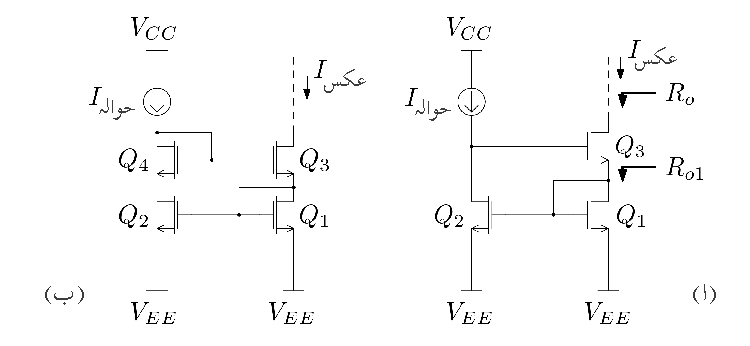
\includegraphics[scale=0.90]{mosfetWilsonCurrentMirror}
\caption{ولسن آئینے کی خارجی مزاحمت}
\label{شکل_تفرقی_ماسفیٹ_ولسن_آئینے_کی_خارجی_مزاحمت}
\end{figure}

شکل \حوالہ{شکل_تفرقی_ماسفیٹ_ولسن_آئینے_کی_خارجی_مزاحمت} الف میں ولسن آئینہ برقی رو دکھایا گیا ہے۔دو جوڑ ٹرانزسٹر سے بنائے گئے ولسن آئینے میں ماسفیٹ استعمال کرنے سے یہ دور حاصل کیا گیا ہے۔شکل \حوالہ{شکل_تفرقی_ماسفیٹ_ولسن_آئینے_کی_خارجی_مزاحمت} ب میں \عددیء{Q_4} کا اضافہ کرتے ہوئے \عددیء{Q_1} اور \عددیء{Q_2} کے \عددیء{V_{DS}} برابر کر دئے گئے ہیں۔ایسا کرنے سے ولسن آئینے میں ارلی برقی دباو کا اثر ختم ہو جاتا ہے۔

خارجی مزاحمت حاصل کرنے کی خاطر شکل \حوالہ{شکل_تفرقی_ماسفیٹ_ولسن_آئینے_کی_خارجی_مزاحمت} الف میں \عددیء{Q_3} کے ڈرین پر \عددیء{v_t} لاگو کرتے ہوئے \عددیء{i_t} کا تخمینہ لگاتے ہیں۔خارجی مزاحمت  ان دونوں کی شرح کو کہتے ہیں۔آئیں پہلے \عددیء{Q_1} پر غور کریں۔

صفحہ \حوالہصفحہ{شکل_ٹرانزسٹر_سے_ڈایوڈ_کا_حصول} پر شکل \حوالہ{شکل_ٹرانزسٹر_سے_ڈایوڈ_کا_حصول} میں دو جوڑ ٹرانزسٹر کے کلکٹر اور بیس کو آپس میں جوڑ کر ڈایوڈ حاصل کیا گیا ہے۔شکل \حوالہ{شکل_تفرقی_ماسفیٹ_ولسن_آئینے_کی_خارجی_مزاحمت} الف میں \عددیء{Q_1} کو اسی طرز پر جوڑا گیا ہے۔آئیں شکل \حوالہ{شکل_تفرقی_ماسفیٹ_ولسن_آئینے_کی_خارجی_مزاحمت} الف میں \عددیء{Q_1} کا خارجی مزاحمت \عددیء{R_{o1}} حاصل کریں۔\عددیء{R_o} حاصل کرنے کی خاطر \عددیء{Q_1} کے ڈرین پر \عددیء{v_{t1}} لاگو کرتے ہوئے \عددیء{i_t} کا تخمینہ لگاتے ہیں۔شکل \حوالہ{شکل_تفرقی_ماسفیٹ_بطور_ڈایوڈ} میں ایسا کرتے ہوئے  \عددیء{Q_1}  کا باریک اشاراتی مساوی دور بنایا گیا ہے۔چونکہ ڈرین اور گیٹ آپس میں جڑے ہیں لہٰذا  \عددیء{v_{gs1}=v_t} ہے۔یوں
\begin{align*}
i_{t1}&=g_{m1} v_{gs1}+\frac{v_{t1}}{r_{o1}}\\
&=g_{m1} v_{t1}+\frac{v_{t1}}{r_{o1}}
\end{align*}
لکھتے ہوئے
\begin{align}
R_{o1}=\frac{v_{t1}}{i_{t1}}=\frac{r_{o1}}{1+g_{m1} r_{o1}}
\end{align}
حاصل ہوتا ہے۔\عددیء{g_{m} r_o \gg 1} کی بنا پر اس مساوات کو
\begin{align}
R_{o1} \approx \frac{1}{g_{m1}}
\end{align}
لکھا جا سکا ہے۔اس مساوات کے تحت ڈایوڈ کے طرز پر جڑے ماسفیٹ کو مزاحمت \عددیء{\tfrac{1}{g_m}} تصور کیا جا سکتا ہے۔یہ ایک اہم اور عمومی نتیجہ ہے۔ 
\begin{figure}
\centering
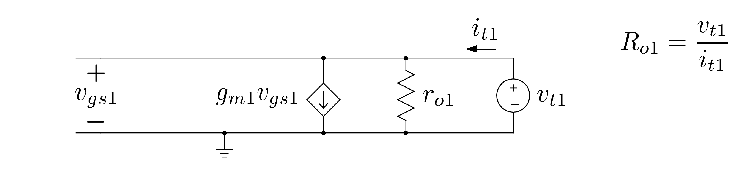
\includegraphics[scale=0.90]{mosfetDiodeConnected}
\caption{ماسفیٹ بطور ڈایوڈ}
\label{شکل_تفرقی_ماسفیٹ_بطور_ڈایوڈ}
\end{figure}

شکل \حوالہ{شکل_تفرقی_ماسفیٹ_ولسن_آئینے_کی_خارجی_مزاحمت} الف میں \عددیء{Q_1} کی جگہ مزاحمت \عددیء{\tfrac{1}{g_{m1}}} جبکہ بقایا ٹرانزسٹروں کے ریاضی نمونہ استعمال کرتے ہوئے شکل \حوالہ{شکل_تفرقی_ماسفیٹ_ولسن_مساوی_دور} حاصل ہوتا ہے۔یہاں رک کر تسلی کر لیں کہ یہی مساوی دور ہے۔ 
\begin{figure}
\centering
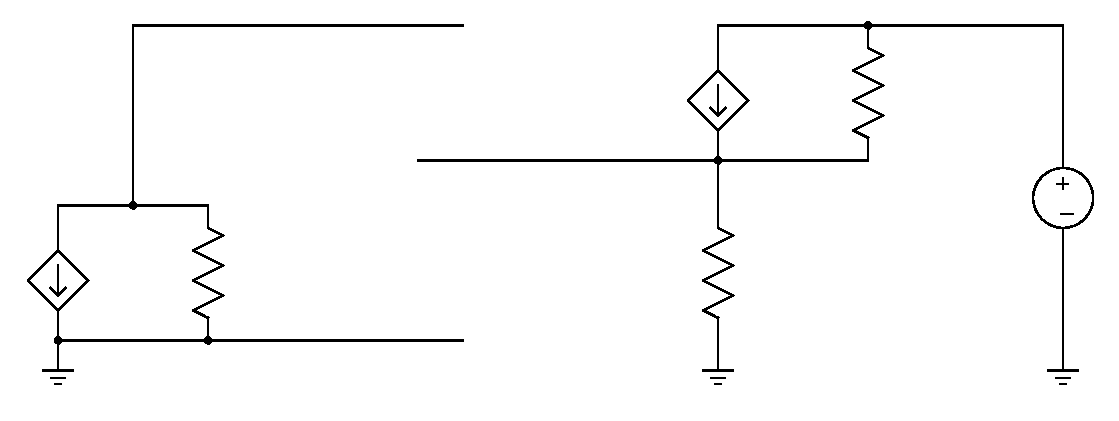
\includegraphics[scale=0.90]{mosfetWilsonCurrentMirrorEquivalent}
\caption{ماسفیٹ ولسن آئینے کا باریک اشاراتی مساوی دور}
\label{شکل_تفرقی_ماسفیٹ_ولسن_مساوی_دور}
\end{figure}

شکل \حوالہ{شکل_تفرقی_ماسفیٹ_ولسن_مساوی_دور} میں \عددیء{Q_1} کے ڈرین پر برقی دباو کو \عددیء{v_1} کہا گیا ہے۔تمام کی تمام \عددیء{i_t} مزاحمت \عددیء{\tfrac{1}{g_{m1}}} سے گزرتی ہے لہٰذا \عددیء{i_t=g_{m1} v_1} کے برابر ہے۔آپ دیکھ سکتے ہیں کہ \عددیء{v_1} دراصل \عددیء{v_{gs2}} ہی ہے لہٰذا
\begin{align}\label{مساوات_تفرقی_ولسن_پہلا_ماسفیٹ}
v_{gs2}=v_{1}=\frac{i_t}{g_{m1}}
\end{align}
لکھا جا سکتا ہے۔یوں \عددیء{Q_2} کے ریاضی نمونہ میں
\begin{align*}
g_{m2} v_{gs2}=\frac{g_{m2} i_t}{g_{m1}}
\end{align*}
کے برابر ہو گا۔آپ دیکھ سکتے ہیں کہ یہی برقی رو \عددیء{r_{o2}} میں برقی زمین سے جوڑ \عددیء{v_2} کی جانب رواں ہے۔یوں
\begin{align*}
v_2=-\frac{g_{m2} r_{o2} i_t}{g_{m1}}
\end{align*}
کے برابر ہے۔چونکہ \عددیء{v_{gs3}=v_2} ہی ہے لہٰذا
\begin{align}\label{مساوات_تفرقی_ماسفیٹ_ولسن_تیسرا_ماسفیٹ}
v_{gs3}=-\frac{g_{m2} r_{o2} i_t}{g_{m1}}
\end{align}
کے برابر ہے۔یوں کرخوف کے قانون برائے برقی رو کی مدد سے
\begin{align*}
i_t&=g_{m3} v_{gs3}+\frac{v_t-v_1}{r_{o3}}\\
&=-\frac{g_{m2} g_{m3} r_{o2} i_t}{g_{m1}}+\frac{v_t-g_{m1} i_t}{r_{o3}}
\end{align*}
لکھا جا سکتا ہے جہاں دوسری قدم پر مساوات \حوالہ{مساوات_تفرقی_ولسن_پہلا_ماسفیٹ} اور مساوات \حوالہ{مساوات_تفرقی_ماسفیٹ_ولسن_تیسرا_ماسفیٹ} کا استعمال کیا گیا۔اس کو
\begin{align*}
i_t+\frac{g_{m2} g_{m3} r_{o2} i_t}{g_{m1}}+\frac{g_{m1} i_t}{r_{o3}}=\frac{v_t}{r_{o3}}
\end{align*}
لکھتے ہوئے
\begin{gather}
\begin{aligned}
R_o=\frac{v_t}{i_t}&=r_{o3}+\frac{g_{m2}g_{m3} r_{o2} r_{o3} }{g_{m1}} +g_{m1}
\end{aligned}
\end{gather}
حاصل ہوتا ہے۔اگر  تمام ماسفیٹ بالکل یکساں ہوں تب \عددیء{g_{m1}=g_{m2}=g_{m3}=g_m} اور \عددیء{r_{o2}=r_{o3}=r_o} لکھا جا سکتا ہے۔ مندرجہ بالا مساوات میں درمیانی جزو بقایا دو اجزاء سے بہت بڑی ہے لہٰذا  پہلی اور آخری اجزاء کو نظرانداز کرتے ہوئے
\begin{gather}
\begin{aligned}
R_o & & \approx g_m r_o^2
\end{aligned} 
\end{gather}
حاصل ہوتا ہے۔
%==============================
\جزوحصہ{منبع دباو کے اثرات سے آزاد منبع رو}
مختلف آئینہ برقی رو پر تبصرے کے دوران یہ تصور کیا گیا کہ \عددیء{I_{\textrm{حوالہ}}} ایک مستقل مقدار ہے جس پر منبع دباو  \عددیء{V_{CC}}اور \عددیء{V_{EE}} کا کوئی اثر نہیں۔آئیں ایک ایسے \اصطلاح{منبع رو}\فرہنگ{منبع رو}\فرہنگ{current source}\حاشیہب{current source} پر غور کریں جس کی پیدا کردہ برقی رو پر  \عددیء{V_{+}}، \عددیء{V_{-}} وغیرہ کا کوئی اثر نہیں ہوتا۔ایسے  منبع رو کو شکل \حوالہ{شکل_تفرقی_ماسفیٹ_منبع_سے_آزاد_پیداکار_برقی_رو} میں دکھایا گیا ہے۔

تمام ماسفیٹ کو افزائندہ تصور کریں۔\عددیء{Q_3} اور \عددیء{Q_4} مل کر منبع برقی رو بناتے ہیں جسے اب تک ہم دیکھتے آ رہے ہیں۔\عددیء{Q_3} اور \عددیء{Q_4} بالکل یکساں ہیں۔یوں \عددیء{I_{D1}=I_{D2}} ہو گا۔آئیں اب \عددیء{Q_1} اور \عددیء{Q_2} پر غور کریں۔\عددیء{Q_1} کا برقی رو \عددیء{I_{D1}} ہی ہے۔اسی طرح \عددیء{Q_2} کا برقی رو \عددیء{I_{D2}} ہی ہے۔یوں
\begin{align*}
I_{D1}&=\frac{k_n'}{2} \left(\frac{W}{L} \right)_1 \left(V_{GS1}-V_t \right)^2\\
I_{D2}&=\frac{k_n'}{2} \left(\frac{W}{L} \right)_2 \left(V_{GS2}-V_t \right)^2
\end{align*} 
ان دونوں برقی رو کو برابر لکھتے ہوئے
\begin{align}\label{مساوت_تفرقی_منبع_سے_پاک_کے_برقی_رو}
\frac{k_n'}{2} \left(\frac{W}{L} \right)_1 \left(V_{GS1}-V_t \right)^2=\frac{k_n'}{2} \left(\frac{W}{L} \right)_2 \left(V_{GS2}-V_t \right)^2
\end{align}
حاصل ہوتا ہے۔ساتھ ہی ساتھ شکل کو دیکھتے ہوئے ہم لکھ سکتے ہیں
\begin{align}\label{مساوات_تفرقی_منبع_سے_پاک_کے_تعلق}
V_{GS1}=V_{GS2}+I_{D2} R
\end{align}
مساوات \حوالہ{مساوات_تفرقی_منبع_سے_پاک_کے_تعلق} کو مساوات \حوالہ{مساوت_تفرقی_منبع_سے_پاک_کے_برقی_رو} میں پُر کرتے ہوئے \عددیء{R} کے لئے حل کرتے ہیں۔
\begin{align*}
\frac{k_n'}{2} \left(\frac{W}{L} \right)_1 \left(V_{GS2}+I_{D2} R-V_t \right)^2=\frac{k_n'}{2} \left(\frac{W}{L} \right)_2 \left(V_{GS2}-V_t \right)^2
\end{align*}
دونوں اطراف کا  جزر    لیتے ہوئے
\begin{align*}
\sqrt{\left(\frac{W}{L} \right)_1} \left(V_{GS2}+I_{D2} R-V_t \right)=\sqrt{\left(\frac{W}{L} \right)_2} \left(V_{GS2}-V_t \right)
\end{align*}
سے
\begin{align*}
R=\frac{V_{GS2}-V_t}{I_{D2}} \left[ \sqrt{\frac{\left(\frac{W}{L} \right)_2}{\left(\frac{W}{L} \right)_1}} -1\right]
\end{align*}
حاصل ہوتا ہے۔\عددیء{I_{D2}} کی مساوات سے 
\begin{align*}
V_{GS2}-V_t=\sqrt{\frac{I_{D2}}{\frac{k_{n2}}{2}}}
\end{align*}
لکھا جا سکتا ہے۔یوں
\begin{align}
R=\frac{\sqrt{2}}{\sqrt{k_{n2} I_{D2}}} \left[ \sqrt{\frac{\left(\frac{W}{L} \right)_2}{\left(\frac{W}{L} \right)_1}} -1\right]
\end{align}
 حاصل ہوتا ہے۔اس قیمت کی مزاحمت اس بات کو یقینی بنائے گی کہ \عددیء{I_{D1}=I_{D2}} ہوں گے۔چونکہ \عددیء{R \ge 0} ہوتا ہے لہٰذا
\begin{align*}
\left(\frac{W}{L} \right)_2 \ge \left(\frac{W}{L} \right)_1
\end{align*}
ہو گا۔\عددیء{Q_1} کے برقی رو کے عکس لینے کی خاطر  \عددیء{V_{GS1}} برقی دباو مزید ماسفیٹ کو دیا جاتا ہے۔شکل میں یوں \عددیء{Q_6} سے \عددیء{I_{\textrm{عکس}}} حاصل کیا گیا ہے جسے \عددیء{I_{O6}} سے ظاہر کیا گیا ہے۔اسی طرح  \عددیء{Q_4} کے برقی رو کے عکس لینے کی خاطر  \عددیء{V_{GS4}} برقی دباو مزید ماسفیٹ کو دیا جاتا ہے۔شکل میں یوں \عددیء{Q_5} سے \عددیء{I_{\textrm{عکس}}} حاصل کیا گیا ہے جسے \عددیء{I_{O5}} سے ظاہر کیا گیا ہے۔

\عددیء{I_{D1}} اور \عددیء{I_{D2}} اس وقت تک \عددیء{V_{+}} اور \عددیء{V_{-}} کے اثرات سے آزاد رہتے ہیں جب تک \عددیء{Q_2} اور \عددیء{Q_3} افزائندہ رہیں۔یاد رہے کہ \عددیء{Q_1} کا گیٹ اور اس کا ڈرین آپس میں جڑے ہیں لہٰذا یہ ہر صورت افزائندہ ہی رہتا ہے۔اسی طرح \عددیء{Q_4} کا گیٹ اور ڈرین بھی آپس میں جڑے ہیں لہٰذا یہ ماسفیٹ بھی ہر صورت افزائندہ ہی رہتا ہے۔

اور \عددیء{Q_4} کا \عددیء{V_{SG4}}
\begin{figure}
\centering
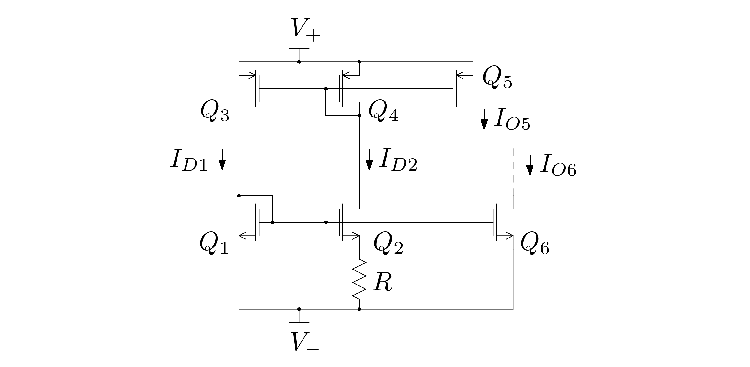
\includegraphics[scale=0.90]{supplyIndependentCurrentSource}
\caption{منبع دباو کے اثرات سے پاک منبع رو}
\label{شکل_تفرقی_ماسفیٹ_منبع_سے_آزاد_پیداکار_برقی_رو}
\end{figure}
%==============================
\حصہ{ماسفیٹ کیسکوڈ تفرقی ایمپلیفائر}
شکل \حوالہ{شکل_تفرقی_ماسفیٹ_کیسکوڈ} میں ماسفیٹ سے بنایا گیا کیسکوڈ تفرقی ایمپلیفائر دکھایا گیا ہے جس میں ولسن آئینے کو بطور برقی بوجھ استعمال کیا گیا ہے۔ولسن آئینے کی خارجی مزاحمت گزشتہ حصے میں حاصل کی گئی۔آئیں کیسکوڈ کی خارجی مزاحمت بھی حاصل کریں۔ایسا کرنے کی خاطر \عددیء{Q_{a4}} کے ڈرین پر \عددیء{v_t} مہیا کرتے ہوئے \عددیء{i_t} کا تخمینہ لگائیں گے۔\عددیء{\tfrac{v_t}{i_t}} خارجی مزاحمت ہو گا۔
\begin{figure}
\centering
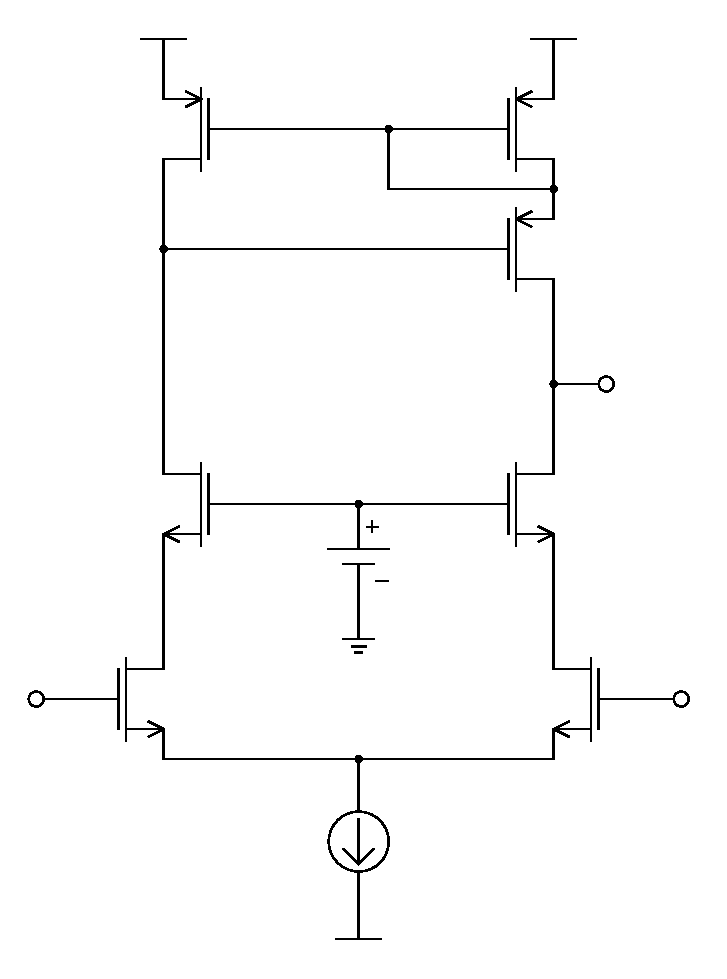
\includegraphics[scale=0.90]{mosfetCascodeWilsonLoaded}
\caption{ماسفیٹ کیسکوڈ تفرقی ایمپلیفائر}
\label{شکل_تفرقی_ماسفیٹ_کیسکوڈ}
\end{figure}

شکل \حوالہ{شکل_تفرقی_ماسفیٹ_کیسکوڈ_مزاحمت} میں کیسکوڈ ایمپلیفائر کا مطلوبہ حصہ دکھایا گیا ہے۔ساتھ ہی دونوں ماسفیٹ کے باریک اشاراتی ریاضی نمونہ استعمال کرتے ہوئے مساوی دور بھی بنایا گیا ہے جہاں تفرقی داخلی اشارہ \عددیء{v_d=0} رکھا گیا ہے۔چونکہ \عددیء{Q_{a2}} کا سورس اور گیٹ دونوں برقی زمین پر ہیں لہٰذا \عددیء{v_{gs2}=0} ہے۔یوں \عددیء{g_{m2} v_{gs2}=0} ہو گا۔اس طرح \عددیء{Q_{a2}} کی جگہ صرف \عددیء{r_{o2}} نسب کیا جا سکتا تھا۔آپ دیکھ سکتے ہیں کہ \عددیء{i_t} تمام کی تمام \عددیء{r_{o2}} سے گزرتی ہے لہٰذا \عددیء{v_1=i_t r_{o2}} کے برابر ہے۔شکل سے صاف ظاہر ہے کہ \عددیء{v_{gs4}=-v_1} ہے یوں
\begin{gather}
\begin{aligned}\label{مساوات_تفرقی_ماسفیٹ_کیسکوڈ_خارجی_مزاحمت}
v_1&=i_t r_{o2}\\
v_{gs4}&=-i_t r_{o2}
\end{aligned}
\end{gather}
لکھا جا سکتا ہے۔کرخوف کے قانون برائے برقی رو کی مدد سے
\begin{align*}
i_t&=g_{m4} v_{gs4}+\frac{v_t-v_1}{r_{o4}}\\
&=-i_t g_{m4} r_{o2}+\frac{v_t-i_t r_{o2}}{r_{o4}}
\end{align*}
لکھا جا سکتا ہے جہاں دوسری قدم پر مساوات \حوالہ{مساوات_تفرقی_ماسفیٹ_کیسکوڈ_خارجی_مزاحمت} کا سہارا لیا گیا۔اس مساوات کو
\begin{align*}
i_t+i_t g_{m4} r_{o2}+\frac{i_t r_{o2}}{r_{o4}}=\frac{v_t}{r_{o4}}
\end{align*}
لکھتے ہوئے
\begin{align}
R_o=\frac{v_t}{i_t}=r_{o4}+g_{m4} r_{o2} r_{o4}+r_{o2}
\end{align}
حاصل ہوتا ہے جہاں درمیانی جزو بقایا دو اجزاء سے بہت بڑی ہے لہٰذا پہلی اور تیسری جزو کو نظرانداز کیا جا سکتا ہے۔ساتھ ہی ساتھ اگر تمام ماسفیٹ بالکل یکساں ہوں تب \عددیء{g_{m2}=g_{m4}=g_m} اور \عددیء{r_{o2}=r_{o4}=r_o} لکھا جا سکتا ہے۔یوں
\begin{align}
R_o=g_{m} r_o^2
\end{align}
حاصل ہوتا ہے۔شکل \حوالہ{شکل_تفرقی_ماسفیٹ_کیسکوڈ} میں اس خارجی مزاحمت کو دکھایا گیا ہے۔کیسکوڈ تفرقی جوڑے کی خارجی مزاحمت اور ولسن آئینے کی خارجی مزاحمت آپس میں متوازی جڑے ہیں لہٰذا ان کا مجموعہ \عددیء{\frac{g_m r_o^2}{2}} ہو گا۔یوں کیسکوڈ  تفرقی ایمپلیفائر کا خارجی اشارہ
\begin{align*}
v_o =\left(g_m \frac{v_d}{2}+ g_m \frac{v_d}{2}\right) \left(g_m r_o^2 \right)
\end{align*} 
ہو گا جس سے
\begin{align}
A_d=\frac{1}{2} g_m^2 r_o^2
\end{align}
حاصل ہوتا ہے۔
\begin{figure}
\centering
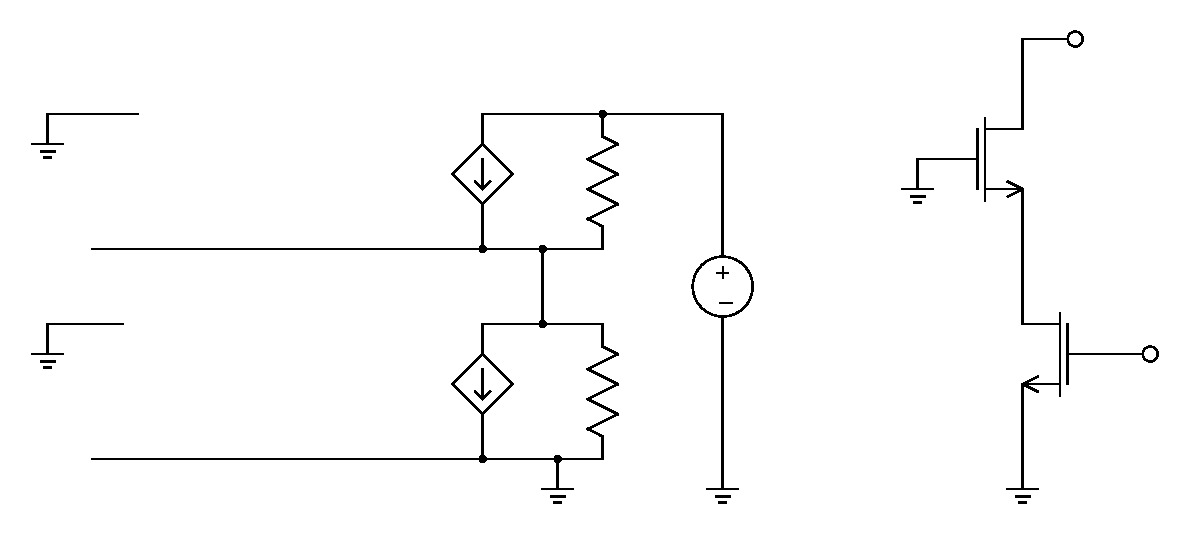
\includegraphics[scale=0.90]{mosfetCascodeOutputResistance}
\caption{ماسفیٹ کیسکوڈ  کا خارجی مزاحمت}
\label{شکل_تفرقی_ماسفیٹ_کیسکوڈ_مزاحمت}
\end{figure}
%======================================
%==========================================

\newpage
\حصہء{سوالات}

\ابتدا{سوال}
شکل \حوالہ{شکل_تفرقی_جوڑے_کی_بنیادی_ساخت} میں  \عددیء{V_{CC}=\SI{10}{\volt}}، \عددیء{V_{EE}=\SI{-10}{\volt}}،\عددیء{I=\SI{0.5}{\milli \ampere}}، \عددی{R_C=\SI{15}{\kilo \ohm}} اور \عددی{\alpha=0.97} ہیں۔\عددی{v_{B1}=v_{B2}=\SI{-2}{\volt}} کی صورت میں \عددی{v_o} حاصل کریں۔مشترکہ اشارے کی بلند تر قیمت حاصل کریں۔

جواب:\عددیء{\SI{0}{\volt}}، \عددی{V_{CM}\le \SI{3.15}{\volt}}
\انتہا{سوال}
%===================
\ابتدا{سوال}\شناخت{سوال_تفرقی_جوڑا_بنیادی_کارکردگی}
شکل \حوالہ{شکل_تفرقی_جوڑے_کی_بنیادی_ساخت} میں  \عددیء{V_{CC}=\SI{10}{\volt}}، \عددیء{V_{EE}=\SI{-10}{\volt}}،\عددیء{I=\SI{0.25}{\milli \ampere}}، \عددی{R_C=\SI{15}{\kilo \ohm}} اور \عددی{\alpha=0.97} ہیں۔\عددی{v_{B1}=\SI{-2}{\volt}} اور \عددی{v_{B2}=\SI{-3.1}{\volt}} کی صورت میں \عددی{v_o} حاصل کریں۔

جواب:\عددیء{\SI{7.35}{\volt}}
\انتہا{سوال}
%===========
\ابتدا{سوال}
مساوات \حوالہ{مساوات_تفرقی_دوسری_رو_بالمقابل_تفرقی_دباو} حاصل کریں۔
\انتہا{سوال}
%========================
\ابتدا{سوال}
سوال \حوالہ{سوال_تفرقی_جوڑا_بنیادی_کارکردگی} میں \عددی{v_{B1}=\SI{-2.1}{\volt}} اور \عددی{v_{B2}=\SI{-2.101}{\volt}} کی صورت میں \عددی{v_o} حاصل کریں۔ 
\انتہا{سوال}
%===============
\ابتدا{سوال}
مساوات \حوالہ{مساوات_تفرقی_جوڑا_دوسری_برقی_رو} حاصل کریں۔
\انتہا{سوال}
%=================
\ابتدا{سوال}
\عددی{i_{DS1}} کو \عددی{i_{DS2}} پر تقسیم کرتے ہوئے مساوات \حوالہ{مساوات_تفرقی_رقبے_میں_فرق_سے_دوسری_برقی_رو} حاصل کریں۔
\انتہا{سوال}
%============================
\ابتدا{سوال}
مساوات \حوالہ{مساوات_تفرقی_رقبے_میں_فرق_سے_داخلی_انحرافی_برقی_دباو} حاصل کریں۔
\انتہا{سوال}
%================
\ابتدا{سوال}
اگر شکل \حوالہ{شکل_تفرقی_حسابی_ایمپلیفائر_بنیادی_دور} میں \عددیء{Q_{11}} کا لبریزی برقی رو \عددیء{4 \times I_S} ہو تب \عددی{v_O=\SI{0}{\volt}} حاصل کرنے کے لئے درکار  \عددیء{R_{B8}} حاصل کریں۔

جواب:\عددیء{\SI{25.2}{\kilo \ohm}}
\انتہا{سوال}
%==================
\ابتدا{سوال}\شناخت{سوال_تفرقی_حسابی_اندرونی_دور_الف}
شکل \حوالہ{شکل_تفرقی_حسابی_ایمپلیفائر_بنیادی_دور} میں \عددیء{V_{CC}=\SI{15}{\volt}}، \عددیء{V_{EE}=\SI{-15}{\volt}} ہے۔تمام ٹرانزسٹر کا \عددیء{\beta =100} ہے۔ \عددیء{Q_9} کا \عددیء{I_{\textrm{حوالہ}}=\SI{1}{\milli \ampere}} درکار ہے۔\عددیء{R_{C9}} حاصل کریں۔\عددیء{I_{C5}} کا شامل کرتے ہوئے \عددیء{V_{C2}=V_{C3}=\SI{7.5}{\volt}} حاصل کرنے کی خاطر \عددیء{R_{C2}} حاصل کریں۔\عددیء{V_{C5}=\SI{10}{\volt}} حاصل کرنے کی خاطر \عددیء{R_{C5}} حاصل کریں۔\عددیء{I_{C7}=\SI{0.5}{\milli \ampere}} کے لئے درکار \عددیء{R_{E7}} حاصل کریں۔\عددیء{v_O=\SI{0}{\volt}} اور \عددیء{I_{E8}=\SI{6}{\milli \ampere}} حاصل کرنے کے لئے درکار \عددیء{R_{B8}} اور \عددیء{R_{E8}} حاصل کریں۔

جوابات:\عددیء{R_{C9}=\SI{28.6}{\kilo \ohm}}، \عددیء{R_{C2}=\SI{4.2857}{\kilo \ohm}}، \عددیء{R_{C5}=\SI{3.33}{\kilo \ohm}}، \عددیء{R_{E7}=\SI{8.6}{\kilo \ohm}}، \عددیء{R_{B8}=\SI{31.4}{\kilo \ohm}} اور \عددیء{R_{E8}=\SI{2.5}{\kilo \ohm}}
\انتہا{سوال}
%========================
\ابتدا{سوال}
سوال \حوالہ{سوال_تفرقی_حسابی_اندرونی_دور_الف} میں \عددیء{R_{C5}} کی کس قیمت پر \عددیء{Q_5} غیر افزائندہ ہو جائے گا۔یاد رہے کہ ٹرانزسٹر اس وقت غیر افزائندہ ہوتا ہے جب اس کا \عددیء{V_{CB} \le \SI{0.5}{\volt}} ہو۔

جواب:\عددیء{\SI{5.333}{\kilo \ohm}} 
\انتہا{سوال}
%=======================
\ابتدا{سوال}
سوال \حوالہ{سوال_تفرقی_حسابی_اندرونی_دور_الف} میں چاروں ایمپلیفائر کے داخلی مزاحمت حاصل کریں۔

جوابات:\عددیء{\SI{2}{\mega \ohm}}، \عددیء{\SI{3.33}{\kilo \ohm}}، \عددیء{\SI{860}{\kilo \ohm}} اور \عددیء{\SI{250}{\kilo \ohm}}
\انتہا{سوال}
%================
\ابتدا{سوال}
سوال \حوالہ{سوال_تفرقی_حسابی_اندرونی_دور_الف} میں  تمام تفرقی ایمپلیفائر کی افزائش حاصل کرتے ہوئے کُل افزائش \عددیء{A_d} حاصل کریں۔

جوابات:\عددیء{\SI{12}{\volt \per \volt}}، \عددیء{\SI{-100}{\volt \per \volt}}، \عددیء{\SI{-3.65}{\volt \per \volt}}، \عددیء{\SI{1}{\volt \per \volt}}، \عددیء{A_d=\SI{4380}{\volt \per \volt}}
\انتہا{سوال}
%=======================
\ابتدا{سوال}
سوال \حوالہ{سوال_تفرقی_حسابی_اندرونی_دور_الف} میں \عددیء{v_d=\SI{200}{\micro \volt}} ہے۔پہلے، دوسرے، تیسرے اور چوتھے تفرقی ایمپلیفائر کے خارجی اشارے دریافت کریں۔

جواب:\عددیء{\SI{2.4}{\milli \volt}}، \عددیء{\SI{0.24}{\volt}}، \عددیء{\SI{0.876}{\volt}}، \عددیء{\SI{0.876}{\volt}}
\انتہا{سوال}
%==================
\ابتدا{سوال}
سوال \حوالہ{سوال_تفرقی_حسابی_اندرونی_دور_الف}  میں \عددیء{A_i} حاصل کرتے ہوئے \عددیء{A_d} کی قیمت حاصل کریں۔
\انتہا{سوال}
%=====================
\ابتدا{سوال}
صفحہ \حوالہصفحہ{شکل_تفرقی_وائڈلر_آئینہ_مثال} پر شکل \حوالہ{شکل_تفرقی_وائڈلر_آئینہ_مثال} ب میں \عددیء{R_{\textrm{حوالہ}}=\SI{10}{\kilo \ohm}} جبکہ \عددیء{R_E=\SI{12}{\kilo \ohm}} ہیں۔\عددیء{I_{\textrm{عکس}}} حاصل کریں۔

جواب:\عددیء{I_{\textrm{حوالہ}}=\SI{0.83}{\milli \ampere}} اور  \عددیء{I_{\textrm{عکس}}=\SI{9.3}{\micro \ampere}} حاصل ہوتے ہیں۔اس جواب کو گراف کی مدد سے با آسانی حاصل کیا جا سکتا ہے۔اس کے علاوہ بار بار حل کرتے ہوئے بہتر سے بہتر جواب حاصل کرتے ہوئے بھی جواب حاصل کیا جا سکتا ہے۔ 
\انتہا{سوال}
%======================
\ابتدا{سوال}
صفحہ \حوالہصفحہ{شکل_تفرقی_ولسن_آئینہ} پر شکل \حوالہ{شکل_تفرقی_ولسن_آئینہ} الف میں ولسن آئینہ دکھایا گیا ہے۔ٹرانزسٹر کا \عددیء{\beta=100} جبکہ ارلی برقی دباو \عددیء{V_A=\SI{150}{\volt}} ہے۔\عددیء{I_{\textrm{حوالہ}}=\SI{1.5}{\milli \ampere}} کی صورت میں  خارجی مزاحمت \عددیء{R_o} حاصل کریں۔

جواب:\عددیء{r_o=\SI{100}{\kilo \ohm}}، \عددیء{R_o=\SI{5}{\mega \ohm}}
\انتہا{سوال}
%=================
\ابتدا{سوال}
صفحہ \حوالہصفحہ{شکل_تفرقی_سادہ_آئینے_کی_خارجی_مزاحمت} پر شکل \حوالہ{شکل_تفرقی_سادہ_آئینے_کی_خارجی_مزاحمت} میں ماسفیٹ ولسن آئینہ دکھایا گیا ہے۔\عددیء{V_A=\SI{50}{\volt}} اور \عددیء{k_n=\SI{0.4}{\milli \ampere \per \squared \volt}} لیتے ہوئے \عددیء{I_{DS}=\SI{1.5}{\milli \ampere}} پر  آئینے کی خارجی مزاحمت \عددیء{R_o} اور افزائش \عددیء{A_d} حاصل کریں۔

جواب:\عددیء{R_o=\SI{1.22}{\mega \ohm}}، \عددیء{A_d=\SI{666}{\volt \per \volt}}
\انتہا{سوال}
%==================
\ابتدا{سوال}
صفحہ \حوالہصفحہ{شکل_تفرقی_کیسکوڈ} پر شکل \حوالہ{شکل_تفرقی_کیسکوڈ} میں تفرقی کیسکوڈ ایمپلیفائر دکھایا گیا ہے۔اگر \عددیء{\beta=100} اور \عددیء{V_A=\SI{200}{\volt}} ہوں تب \عددیء{A_d} کی قیمت کیا ہو گی؟ اگر \عددیء{v_d=0.00002 \sin \omega t} ہو تب \عددیء{v_o} کیا ہو گا؟

جوابات:\عددیء{A_d=\SI{267}{\kilo \volt \per \volt}}، \عددیء{v_o=5.34 \sin \omega t} 
\انتہا{سوال}
%==============

